\documentclass[11pt, oneside]{book}   	% use "amsart" instead of "article" for AMSLaTeX format
% !TEX encoding = UTF-8 Unicode
\usepackage{text_RU}
\newcommand{\LongTitle}{Всё пошло не так: Erlang в гневе}
\newcommand{\ShortTitle}{Erlang в гневе}
\newcommand{\HandsOnTitle}{Тренировочные задания}
\newcommand{\ReviewTitle}{Вопросы для закрепления материала}
\newcommand{\OpenEndedTitle}{Открытые вопросы}
\newcommand\NamedRef[1]{\ref{#1} <<\nameref{#1}>>}

%%% Cover

%\title{Stuff Goes Bad:\protect\\ Erlang in Anger}
%\author{
\includegraphics[width=150pt]{heroku-logo-light.pdf}\\
%Fred Hébert}

%\date{}							% Activate to display a given date or no date

\begin{document}
%\maketitle

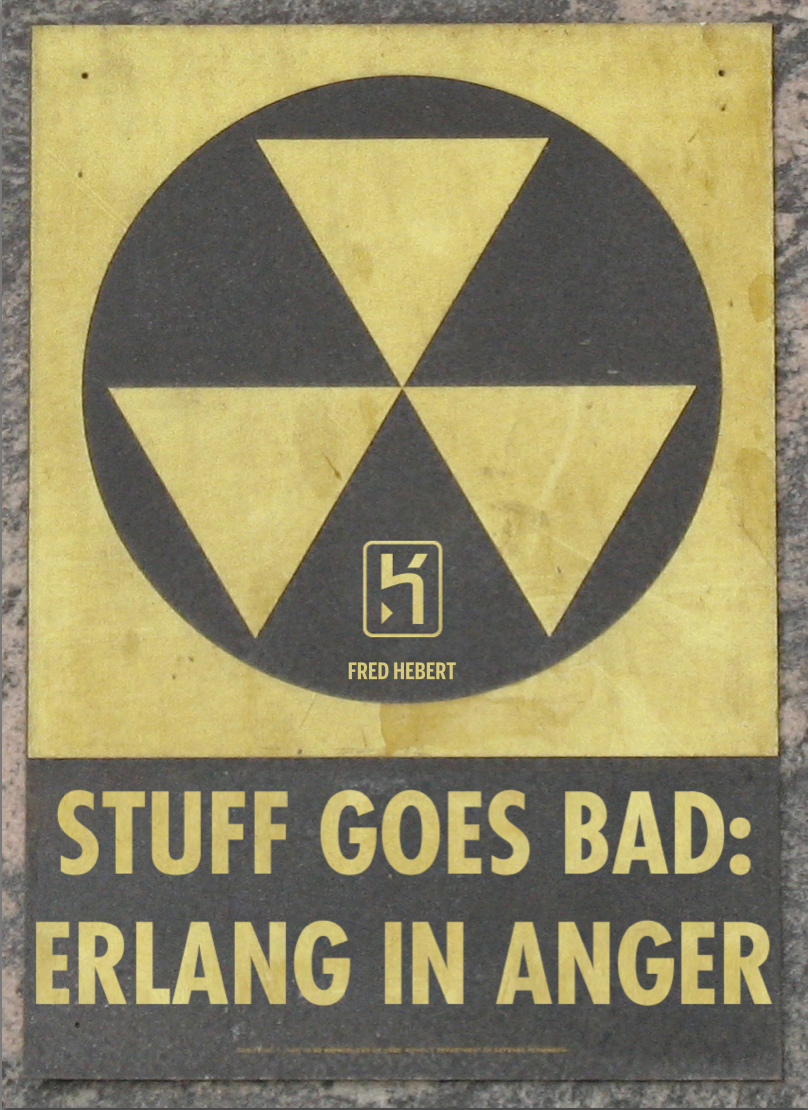
\includepdf[fitpaper=true]{graphics/cover.pdf}

%%% Copyright page
\clearpage
\thispagestyle{fancy}

\fancyhf{} % remove everything
\renewcommand{\headrulewidth}{0pt} % remove lines as well
\renewcommand{\footrulewidth}{0pt}

\vspace*{\fill}


\begin{center}
\includegraphics[width=100pt]{by-nc-sa.eps}
\end{center}

\begin{center}
\emph{\LongTitle} под авторством Fred Hébert и компании Heroku распространяются 
на условиях \href{http://creativecommons.org/licenses/by-nc-sa/4.0/}{Creative 
	Commons Attribution-NonCommercial-ShareAlike 4.0 International License}.
\end{center}

%Thanks for the additional work, reviewing, and/or editing done by:
Благодарность за дополнительную работу, вычитку и редактирование:

\emph{Jacob Vorreuter}, \emph{Seth Falcon}, \emph{Raoul Duke}, \emph{Nathaniel Waisbrot}, \emph{David Holland}, \emph{Alisdair Sullivan}, \emph{Lukas Larsson}, \emph{Tim Chevalier}, \emph{Paul Bone}, \emph{Jonathan Roes}, и \emph{Roberto Aloi}.

\null
\vfill
%\vspace*{\fill}
%The cover image is a modified version of 
Изображение на обложке является изменённой версией
	\href{http://www.freeimages.com/photo/533163}{ядерного убежища} под авторством
	\href{http://www.freeimages.com/profile/drouu}{drouu} с сайта
	\href{http://sxc.hu}{sxc.hu}.
\cfoot{\emph{v1.0.3}}
\rfoot{\emph{2014-10-28}}


%% License as of Monday, August 18, 2014:
%%
%% you may use any of my photos, original or modified, for any purpose whatsoever (personal, non-profit, or commercial; for web or print). you do not need to contact me prior to or after using one of my photos, though a comment or note is always appreciated if you have the opportunity.
%%
%% you may not claim ownership or copyright of my photos. seriously, i have an orbital karma gun and i'm not afraid to use it.

\clearpage
%%%
\pagenumbering{roman}
\setcounter{page}{1}

\tableofcontents

\listoffigures

%% Colors of figure refs for text
\hypersetup{linkcolor=violet}

\chapter*{Вступление}
\markboth{\MakeUppercase{Вступление}}{}
\addcontentsline{toc}{chapter}{Вступление}
\label{chap:introduction}
\pagenumbering{arabic}
\setcounter{page}{1}


\section*{О выполнении приложений}
%\addcontentsline{toc}{section}{On Running Software}
\label{sec:on-running-software}

%There's something rather unique in Erlang in how it approaches failure compared to most other programming languages. There's this common way of thinking where the language, programming environment, and methodology do everything possible to prevent errors. Something going wrong at run-time is something that needs to be prevented, and if it cannot be prevented, then it's out of scope for whatever solution people have been thinking about.
В Erlang есть кое-что уникальное в его подходе к сбоям, если сравнить его с большинством других языков. Существует такой общепринятый ход мыслей, при следованию которому и сам язык, и окружение, в котором работает программист, и методология делают всё возможное, чтобы предотвратить ошибки. Если во время исполнения что-то может пойти не так, то это нужно предотвратить, а если предотвращение невозможно, то оно выходит за пределы любого другого решения, о котором могли бы подумать люди.

%The program is written once, and after that, it's off to production, whatever may happen there. If there are errors, new versions will need to be shipped.
Программа пишется один раз и затем отдаётся на производство (\emph{production}), что бы там с ней ни произошло. Если случатся ошибки, то придётся приготовить и доставить заказчику новые версии.

%Erlang, on the other hand, takes the approach that failures will happen no matter what, whether they're developer-, operator-, or hardware-related. It is rarely practical or even possible to get rid of all errors in a program or a system.\footnote{life-critical systems are usually excluded from this category} If you can deal with some errors rather than preventing them at all cost, then most undefined behaviours of a program can go in that "deal with it" approach.
Erlang, с другой стороны, использует такой подход, при котором сбои считаются неизбежными, независимо от того, что явилось их причиной --- разработчик, оператор или аппаратное обеспечение. Редко считается практичным избавляться от всех ошибок в программе или системе\footnote{Обычно в эту категорию не входят жизненно-важные системы} Если вы можете справиться с ошибками вместо того, чтобы любой ценой их не допустить, то подавляющее количество неожиданных поведений программы может быть разрешено с помощью этого подхода <<справься с ситуацией сам>>.

%This is where the "Let it Crash"\footnote{Erlang people now seem to favour "let it fail", given it makes people far less nervous.} idea comes from: Because you can now deal with failure, and because the cost of weeding out all of the complex bugs from a system before it hits production is often prohibitive, programmers should only deal with the errors they know how to handle, and leave the rest for another process (a supervisor) or the virtual machine to deal with.
Вот откуда появилась известная идея <<Дай ему упасть>> (\emph{Let it crash})\footnote{Хотя люди из мира Erlang чаще предпочитают альтернативное <<дай ему завершиться неудачей>>, поскольку такое словосочетание меньше нервирует других людей.}: Потому что вы теперь готовы справиться с неудачным завершением работы алгоритма, и поскольку стоимость выведения всех сложных ошибок из системы до момента её сдачи часто является заоблачной, программисты должны помнить и обрабатывать только те ошибки, к которым они готовы, а остальные ситуации позволить решать другому процессу (наблюдателю) или виртуальной машине.

%Given that most bugs are transient\footnote{131 out of 132 bugs are transient bugs (they're non-deterministic and go away when you look at them, and trying again may solve the problem entirely), according to Jim Gray in \href{http://www.hpl.hp.com/techreports/tandem/TR-85.7.html}{Why Do Computers Stop and What Can Be Done About It?}}, simply restarting processes back to a state known to be stable when encountering an error can be a surprisingly good strategy.
Поскольку большая часть ошибок являются временными\footnote{131 из 132 ошибок являются временными (они недетерминированны и исчезают, как только вы на них пристально посмотрите, а повторная попытка сделать то же самое часто завершается успешно), согласно Jim Gray в его статье \href{http://www.hpl.hp.com/techreports/tandem/TR-85.7.html}{Почему компьютеры останавливаются и что с этим делать?} (на английском).}, простой перезапуск процессов в состояние, известное ранее как стабильное, при обнаружении ошибки, может оказаться удивительно удачной стратегией.

%Erlang is a programming environment where the approach taken is equivalent to the human body's immune system, whereas most other languages only care about hygiene to make sure no germ enters the body. Both forms appear extremely important to me. Almost every environment offers varying degrees of hygiene. Nearly no other environment offers the immune system where errors at run time can be dealt with and seen as survivable.
Erlang является программным окружением, в котором выбранный подход аналогичен иммун\-ной системе человеческого тела, когда большая часть языков программирования только беспоко\-ятся о гигиене, и блокируют доступ бактерий к телу. Обе формы кажутся мне очень важными. Почти любое окружение предлагает различные степени гигиены. Но почти никакое из окружений не предлагает аналог иммунной системы, в которой ошибки времени выполнения решаются на месте и расцениваются как некритичные, после которых система продолжает работу.

%Because the system doesn't collapse the first time something bad touches it, Erlang/OTP also allows you to be a doctor. You can go in the system, pry it open right there in production, carefully observe everything inside as it runs, and even try to fix it interactively. To continue with the analogy, Erlang allows you to perform extensive tests to diagnose the problem and various degrees of surgery (even very invasive surgery), without the patients needing to sit down or interrupt their daily activities.
Поскольку система не обрушивается при первом прикосновении чего-нибудь плохого, Erlang/OTP также позволяет вам стать доктором. Вы можете зайти в систему, открыть крышку прямо на производственном сервере, осторожно изучить всё внутри, не прерывая работы, и даже попытаться интерактивно починить его. Чтобы продолжить эту цепочку аналогий, Erlang позволояет вам выполнять широкий спектр тестов для диагностики проблем и разные уровни хирургии (даже очень глубокую хирургию), без необходимости для пациента ложиться на стол, садиться или прерывать его каждодневные обычные дела.

%This book intends to be a little guide about how to be the Erlang medic in a time of war. It is first and foremost a collection of tips and tricks to help understand where failures come from, and a dictionary of different code snippets and practices that helped developers debug production systems that were built in Erlang.
Эта книга задумана стать небольшой инструкцией на тему того, как стать Erlang-доктором во время войны. Это в первую очередь и в основном --- коллекция подсказок и секретов, которые помогут понять, откуда приходят сбои, и набор фрагментов кода и методик, которые уже помогли другим разработчикам при отладке их рабочих систем, построенных на Erlang.



\section*{Для кого эта книга?}
%\addcontentsline{toc}{section}{Who is this for?}
\label{sec:who-is-this-for}

%This book is not for beginners. There is a gap left between most tutorials, books, training sessions, and actually being able to operate, diagnose, and debug running systems once they've made it to production. There's a fumbling phase implicit to a programmer's learning of a new language and environment where they just have to figure how to get out of the guidelines and step into the real world, with the community that goes with it.
Эта книга не предназначена для начинающих. Существует некоторое расстояние между многими существующими уроками, книгами, учебными занятиями и умением управлять, диагностировать и отлаживать работающие системы после того, как они попали в производство (\emph{production}). Есть некий этап неуверенного нащупывания решений, присущий изучению программистом нового языка и окружения, когда им приходится просто разобраться, как выбираться из пошаговых инструкций и идти в реальный мир с сообществом других людей, которое к этому миру прилагается.

%This book assumes that the reader is proficient in basic Erlang and the OTP framework. Erlang/OTP features are explained as I see fit — usually when I consider them tricky — and it is expected that a reader who feels confused by usual Erlang/OTP material will have an idea of where to look for explanations if necessary\footnote{I do recommend visiting \href{http://learnyousomeerlang.com}{Learn You Some Erlang} or the regular \href{http://www.erlang.org/erldoc}{Erlang Documentation} if a free resource is required}.
Эта книга предполагает, что читатель хорошо освоил базовый Erlang и систему OTP. Возможности Erlang/OTP описываются здесь по желанию автора --- обычно когда автор считает, что в данной ситуации кроется некая хитрость --- и ожидается, что читатель, которого вдруг собьёт с толку некоторый материал об Erlang/OTP, знает где искать пояснения при необходимости\footnote{Я рекомендую посетить сайт \href{http://learnyousomeerlang.com}{Изучай Erlang во имя добра} (имеется в продаже \href{http://dmkpress.com/catalog/computer/programming/functional/978-5-97060-086-3/}{русский перевод книги} на сайте издательства ДМК Пресс), а также \href{http://www.erlang.org/erldoc}{Стандартную документацию Erlang}.}.

%What is not necessarily assumed is that the reader knows how to debug Erlang software, dive into an existing code base, diagnose issues, or has an idea of the best practices about deploying Erlang in a production environment\footnote{Running Erlang in a screen or tmux session is \emph{not} a deployment strategy.}.
Вот что не требуется явно, так это то, что читатель должен знать об отладке программ на Erlang, уметь копаться в существующем исходном коде, диагностировать проблемы или иметь представление о лучших практиках установки Erlang-программ в производственном окружении\footnote{Заметьте, что запуск Erlang в экране screen или tmux \emph{не} является стратегией установки программы.}.


\section*{Как читать эту книгу}
%\addcontentsline{toc}{section}{How To Read This Book}
\label{sec:how-to-read-this-book}

%This book is divided in two parts. 
Книга разделена на две части.

%Part \ref{part:writing-applications} focuses on how to write applications. It includes how to dive into a code base (Chapter \ref{chap:how-to-dive-into-a-code-base}), general tips on writing open source Erlang software (Chapter \ref{chap:building-open-source-erlang-software}), and how to plan for overload in your system design (Chapter \ref{chap:overload}).
Часть \ref{part:writing-applications} сосредоточена на методике написания приложений. Она включает рекомендации по работе с существующим исходным кодом (Глава \ref{chap:how-to-dive-into-a-code-base}), общие советы по написанию программ с открытым исходным кодом (\emph{open source}) на языке Erlang (Глава \ref{chap:building-open-source-erlang-software}), и как учитывать чрезвычайную нагрузку в будущем при проектировании вашей системы (Глава \ref{chap:overload}).


%Part \ref{part:diagnosing-applictions} focuses on being an Erlang medic and concerns existing, living systems. It contains instructions on how to connect to a running node (Chapter \ref{chap:connecting}), and the basic runtime metrics available (Chapter \ref{chap:runtime-metrics}). It also explains how to perform a system autopsy using a crash dump (Chapter \ref{chap:crash-dumps}), how to identify and fix memory leaks (Chapter \ref{chap:memory-leaks}), and how to find runaway CPU usage (Chapter \ref{chap:cpu-hogs}). The final chapter contains instructions on how to trace Erlang function calls in production using \otpapp{recon}\footnote{\href{http://ferd.github.io/recon/}{http://ferd.github.io/recon/} — a library used to make the text lighter, and with generally production-safe functions.} to understand issues before they bring the system down (Chapter \ref{chap:tracing}).
Часть \ref{part:diagnosing-applictions} сосредоточена на вашей роли в качестве Erlang-доктора и касается существующих, живых систем. Она содержит инструкции о том, как подключиться к работающему узлу (Глава \ref{chap:connecting}), и перечень доступных во время выполнения метрик (Глава \ref{chap:runtime-metrics}). Здесь также объясняется как выполнить посмертное вскрытие погибшей системы с помощью аварийного дампа (\emph{crash dump}) (Глава \ref{chap:crash-dumps}), как определить и исправить утечки памяти (Глава \ref{chap:memory-leaks}), и как найти украденное процессорное время (Глава \ref{chap:cpu-hogs}). Последняя глава содержит инструкции о том, как трассировать вызовы функций Erlang на живой производственной системе с помощью приложения \otpapp{recon}\footnote{\href{http://ferd.github.io/recon/}{http://ferd.github.io/recon/} — библиотека, содержащая функции в целом безопасные для использования на работающих системах и помогающая сделать текст книги короче и понятнее.} чтобы понять причины проблем до того, как они приведут к падению системы (Глава \ref{chap:tracing}).

%Each chapter is followed up by a few optional exercises in the form of questions or hands-on things to try if you feel like making sure you understood everything, or if you want to push things further.
После каждой главы имеются несколько необязательных упражнений в виде вопросов или задач, которые можно попробовать решить для того, чтобы проверить ваше понимание материала, или если вы хотите узнать чуточку больше по каждой данной теме.
%%%
%%%
%%%

\part{Написание приложений}
\label{part:writing-applications}

\chapter{Как нырять в чужой исходный код}
\label{chap:how-to-dive-into-a-code-base}

%"Read the source" is one of the most annoying things to be told, but dealing with Erlang programmers, you'll have to do it often. Either the documentation for a library will be incomplete, outdated, or just not there. In other cases, Erlang programmers are a bit similar to Lispers in that they will tend to write libraries that will solve their problems and not really test or try them in other circumstances, leaving it to you to extend or fix issues that arise in new contexts.
Один из самых раздражающих комментариев, которые можно услышать в ответ на любой вопрос --- это <<Читай исходники>>, но в случае с Erlang-программистами вам придётся делать это довольно часто. Либо окажется, что документация к библиотеке неполна, устарела или отсутствует. В других случаях Erlang-программисты чем-то подобны программистам на языке Lisp, в том, что они часто пишут библиотеки, решающие их собственную проблему, и не тестируют их в других ситуациях, оставляя вам свободу расширения или удовольствие исправления проблем, которые вылезают при использовании кода в новом контексте.

%It's thus pretty much guaranteed you'll have to go dive in some code base you know nothing about, either because you inherited it at work, or because you need to fix it or understand it to be able to move forward with your own system. This is in fact true of most languages whenever the project you work on is not one you designed yourself.
Таким образом практически гарантированно вам придётся нырять в чьи-то исходные коды, о которых вам ничего не известно, потому что вы унаследовали их на новом месте работы или поскольку вам нужно починить что-то в коде или понять принципы его работы, чтобы продолжить работу над вашей собственной системой. Это утверждение на самом деле истинно для многих языков, когда ваш проект не спроектирован вами самими.

%There are three main types of Erlang code bases you'll encounter in the wild: raw Erlang code bases, OTP applications, and OTP releases. In this chapter, we'll look at each of these and try to provide helpful tips on navigating them.
Есть три основных вида исходных кодов на Erlang, которые могут вам встретиться в дикой природе: базовый Erlang, приложения OTP и релизы OTP. В этой главе мы посмотрим на каждый из них и попробуем предоставить полезные подсказки для навигации по ним.


\section{Ныряем в сырой Erlang}
\label{sec:dive-raw-erlang}

%If you encounter a raw Erlang code base, you're pretty much on your own. These rarely follow any specific standard, and you have to dive in the old way to figure out whatever happens in there.
Если вам встретился исходный код чего-нибудь на базовом (сыром) Erlang, вам остаётся надеяться только на самих себя. Такой код редко следует принятым стандартам и вам придётся нырять в него по-старинке, чтобы попытаться понять, что в коде происходит.

%This means hoping for a \filename{README.md} file or something similar that can point to an entry point in the application, and going from there, or hoping for some contact information that can be used to ask questions to the author(s) of the library.
Это означает надеяться на наличие файла \filename{README.md} или что-то подобное, где можно найти точку входа в приложение, и начать оттуда. Или, может, удастся найти контактные данные и связаться с автором, чтобы задать ему вопросы по его коду.

%Fortunately, you should rarely encounter raw Erlang in the wild, and they are often beginner projects, or awesome projects that were once built by Erlang beginners and now need a serious rewrite. In general, the advent of tools such as \app{rebar}\footnote{\href{https://github.com/rebar/rebar/}{https://github.com/rebar/rebar/} — a build tool briefly introduced in Chapter \ref{chap:building-open-source-erlang-software}} made it so most people use OTP Applications.
К счастью такой код вам может встретиться не так часто, и обычно это работы новичков или отличные проекты, которые были когда-то начаты новичками, а теперь требуют серьёзного переписывания. В общих словах, появление инструментов таких, как \app{rebar}\footnote{\href{https://github.com/rebar/rebar/}{https://github.com/rebar/rebar/} — инструмент для сборки приложений, кратко описанный в Главе \ref{chap:building-open-source-erlang-software}} сделало так, что многие люди начали создавать приложения OTP.


\section{Ныряем в OTP-приложения}
\label{sec:dive-otp-applications}

%Figuring out OTP applications is usually rather simple. They usually all share a directory structure that looks like:
Разбираться с OTP-приложениями обычно несложно. Часто они имеют одинаковую структуру директорий, которая выглядит так:

\begin{VerbatimRaw}
doc/
ebin/
src/
test/
LICENSE.txt
README.md
rebar.config
\end{VerbatimRaw}

%There might be slight differences, but the general structure will be the same.
Могут быть небольшие отличия, но основная структура будет одинакова для всех.

%Each OTP application should contain an \emph{app file}, either \filename{ebin/<AppName>.app} or more often, \filename{src/<AppName>.app.src}\footnote{A build system generates the final file that goes in \filename{ebin}. Note that in these cases, many  \filename{src/<AppName>.app.src} files do not specify modules and let the build system take care of it.}. There are two main varieties of app files:
Каждое приложение OTP должно обязательно содержать \emph{app-файл}, который находится в \filename{ebin/<ИмяПриложения>.app} либо чаще, \filename{src/<ИмяПриложения>.app.src}\footnote{Система сборки генерирует окончательный файл, который затем помещается в папку \filename{ebin}. Заметьте что в этих случаях многие файлы  \filename{src/<ИмяПриложения>.app.src} не перечисляют все модули проекта, а позволяют системе сборки позаботиться об этом.}. Существует два основных вида app-файлов:

\includecode[erlang]{useragent.app.src}

И такой:

\includecode[erlang]{dispcount.app}

%This first case is called a \emph{library application}, while the second case is a regular \emph{application}.
Первый вариант называется \emph{библиотечным приложением}, а второй --- обычным \emph{приложением}.


\subsection{Библиотечные приложения}
\label{subsec:dive-library-applications}

%Library applications will usually have modules named \module{\emph{appname}\_something}, and one module named \module{\emph{appname}}. This will usually be the interface module that's central to the library and contains a quick way into most of the functionality provided.
Библиотечные приложения обычно содержат модули, названные однообразно в стиле \module{\emph{имяприложения}\_чтото}, и один модуль с именем \module{\emph{имяприложения}}. Обычно это интерфейсный модуль, являющийся центральным для всей библиотеки и предоставляет быстрый доступ к имеющимся функциям библиотеки.

%By looking at the source of the module, you can figure out how it works with little effort: If the module adheres to any given behaviour (\module{gen\_server}, \module{gen\_fsm}, etc.), you're most likely expected to start a process under one of your own supervisors and call it that way. If no behaviour is included, then you probably have a functional, stateless library on your hands. For this case, the module's exported functions should give you a quick way to understand its purpose.
Глядя на исходный текст модуля можно понять, как он работает, без особых усилий: если модуль соответствует некоторому данному поведению (например, \module{gen\_server}, \module{gen\_fsm}, и так далее), от вас ожидается запуск процесса под одним из ваших наблюдателей и вызов его стандартным способом. Если поведение не указано, то, вероятнее всего, это функциональная библиотека без состояния. Для таких случаев взгляд на экспортированные функции должен дать вам возможность понять его назначение.


\subsection{Обычные приложения}
\label{subsec:dive-regular-applications}

%For a regular OTP application, there are two potential modules that act as the entry point:
Для обычного приложения OTP потенциально имеются два модуля, которые могут действовать в качестве точки входа: 

\begin{enumerate*}
	\item \module{\emph{имяприложения}}
	\item \module{\emph{имяприложения}\_app}
\end{enumerate*}

%The first file should be similar in use to what we had in a library application (an entry point), while the second one will implement the \module{application} behaviour, and will represent the top of the application's process hierarchy. In some cases the first file will play both roles at once.
Первый файл должен вести себя подобно тому, как он вёл себя в библиотечном приложении (точка входа), тогда как второй будет реализовать поведение \module{application}, и представлять собой верхушку иерархии процессов приложения. В некоторых случаях первый файл будет играть обе роли одновременно.

%If you plan on simply adding the application as a dependency to your own app, then look inside \module{\emph{appname}} for details and information. If you need to maintain and/or fix the application, go for \module{\emph{appname}\_app} instead.
Если вы планируете просто добавить приложение в качестве зависимости для вашей программы, то смотрите внутрь модуля \module{\emph{имяприложения}} для получения подробностей. Если же вам нужно обслуживать и/или исправить что-то в приложении, то вместо этого смотрите модуль \module{\emph{имяприложения}\_app}.

%The application will start a top-level supervisor and return its \emph{pid}. This top-level supervisor will then contain the specifications of all the child processes it will start on its own\footnote{In some cases, the supervisor specifies no children: they will either be started dynamically by some function of the API or in a start phase of the application, or the supervisor is only there to allow OTP environment variables (in the \expression{env} tuple of the app file) to be loaded.}.
Приложение запустит наблюдателя верхнего уровня и возвратит его \emph{идентификатор процесса}. Этот наблюдатель затем будет содержать спецификации всех дочерних процессов, которые он запустит уже самостоятельно\footnote{В некоторых случаях наблюдатель не описывает никаких дочерних процессов: тогда они либо будут запущены динамически с помощью какой-нибудь функции в API, либо на этапе запуска приложения, либо наблюдатель присутствует здесь только для того, чтобы позволить загрузить переменные окружения OTP (из кортежа \expression{env} в app-файле).}.

%The higher a process resides in the tree, the more likely it is to be vital to the survival of the application. You can also estimate how important a process is by the order it is started (all children in the supervision tree are started in order, depth-first). If a process is started later in the supervision tree, it probably depends on processes that were started earlier.
Чем выше процесс находится в дереве наблюдения, тем более вероятно он окажется жизненно важным для работы приложения. Вы также можете оценить важность процесса по порядку их запуска (все подчинённые процессы в дереве наблюдения запускаются по порядку, начиная с самых глубоко вложенных). Если процесс запущен позднее в дереве наблюдения, то вероятно он зависит от ранее запущенных процессов.

%Moreover, worker processes that depend on each other within the same application (say, a process that buffers socket communications and relays them to a finite-state machine in charge of understanding the protocol) are likely to be regrouped under the same supervisor and to fail together when something goes wrong. This is a deliberate choice, as it is usually simpler to start from a blank slate, restarting both processes, rather than trying to figure out how to recuperate when one or the other loses or corrupts its state.
Более того, рабочие процессы, которые зависят друг от друга внутри одного приложения (скажем, процесс, который собирает в буфер данные, прилетающие из сокета, и передаёт их в конечный автомат, который отвечает за разбор протокола) вероятно будут сгруппированы внутри одного наблюдателя и должны падать все вместе, если что-то идёт не так. Это добровольный выбор программиста, поскольку обычно проще начинать работу с чистым состоянием, перезапуская оба процесса вместо того, чтобы пытаться выяснить, как заживить раны, нанесённые утратой или повреждением состояния другим процессом из связки.

%The supervisor restart strategy reflects the relationship between processes under a supervisor:
Стратегия перезапуска процессов наблюдателем отражает отношение между процессами, которые находятся под наблюдением:

\begin{itemize*}
%	\item \expression{one\_for\_one} and \expression{simple\_one\_for\_one} are used for processes that are not dependent upon each other directly, although their failures will collectively be counted towards total application shutdown\footnote{Some developers will use \expression{one\_for\_one} supervisors when \expression{rest\_for\_one} is more appropriate. They require strict ordering to boot correctly, but forget about said order when restarting or if a predecessor dies.}.
	\item \expression{one\_for\_one} и \expression{simple\_one\_for\_one} используются для тех процессов, которые не зависят прямо друг от друга, хотя их отказы посчитаются в пользу полной остановки приложения\footnote{Некоторые разработчики будут использовать наблюдатели \expression{one\_for\_one} когда на самом деле лучше бы подошла стратегия \expression{rest\_for\_one}. Такие процессы требуют строгого порядка при запуске, но забывают об этом порядке, когда дело доходит до перезапуска, или если предыдущий процесс в связке умирает.}.
%	\item \expression{rest\_for\_one} will be used to represent processes that depend on each other in a linear manner.
	\item \expression{rest\_for\_one} будет использован для процессов, которые зависят линейно друг от друга.
%	\item \expression{one\_for\_all} is used for processes that entirely depend on each other.
	\item \expression{one\_for\_all} используется когда в связке процессов все зависят от всех.
\end{itemize*}

%This structure means it is easiest to navigate OTP applications in a top-down manner by exploring supervision subtrees. 
Эта структура означает, что легче всего изучать OTP-приложения сверху вниз, следуя по ветвям деревьев наблюдения.

%For each worker process supervised, the behaviour it implements will give a good clue about its purpose:
Для каждого рабочего процесса под наблюдением поведение, которое он реализует, даст хорошую подсказку о его назначении:

\begin{itemize*}
%	\item a \module{gen\_server} holds resources and tends to follow client/server patterns (or more generally, request/response patterns)
	\item \module{gen\_server} хранит некоторые ресурсы и обычно следует модели поведения клиент/сервер (или, обобщённо, шаблон поведения запрос/ответ)
%	\item a \module{gen\_fsm} will deal with a sequence of events or inputs and react depending on them, as a Finite State Machine. It will often be used to implement protocols.
	\item \module{gen\_fsm} будет обрабатывать последовательность событий или входных данных и реагировать на них следуя модели поведения конечного автомата. Часто конечные автоматы используются для реализации протоколов.
%	\item a \module{gen\_event} will act as an event hub for callbacks, or as a way to deal with notifications of some sort.
	\item \module{gen\_event} будет вести себя как обработчик событий и центр регистрации обратных вызовов, или как способ справиться с уведомлениями какого-нибудь вида.
\end{itemize*}

%All of these modules will contain the same kind of structure: exported functions that represent the user-facing interface, exported functions for the callback module, and private functions, usually in that order.
Все эти модули будут иметь некоторую схожую структуру: экспортированные функции, которые представляют интерфейс пользователя, ещё экспортированные функции, которые реализуют некоторый модуль обратных вызовов (поведение), приватные функции, обычно в таком порядке.

%Based on their supervision relationship and the typical role of each behaviour, looking at the interface to be used by other modules and the behaviours implemented should reveal a lot of information about the program you're diving into.
На основании их отношений в дереве наблюдателя и типичной роли каждого из поведений, глядя на интерфейс, который будет использован другими модулями и реализованные поведения, можно раскрыть много информации о той программе, в которую вы ныряете.


\subsection{Зависимости}
\label{subsec:dive-dependencies}

%All applications have dependencies\footnote{At the very least on the \module{kernel} and \module{stdlib} applications}, and these dependencies will have their own dependencies. OTP applications usually share no state between them, so it's possible to know what bits of code depend on what other bits of code by looking at the app file only, assuming the developer wrote them in a mostly correct manner. Figure~\ref{fig:app-deps} shows a diagram that can be generated from looking at app files to help understand the structure of OTP applications.
Все приложения имеют зависимости\footnote{Как минимум --- это зависимость от приложений \module{kernel} и \module{stdlib}.}, и эти зависимости могут в свою очередь тоже иметь зависимости. Приложения OTP обычно не разделяют состояния между собой, так что нельзя узнать, какой код зависит от какого просто глядя на app-файл, и предполагая, что они написаны автором в самой корректной манере. Рисунок~\ref{fig:app-deps} показывает диаграмму, которая может быть построена глядя на app-файлы, чтобы помочь лучше понять структуру OTP-приложений.


\begin{figure}
  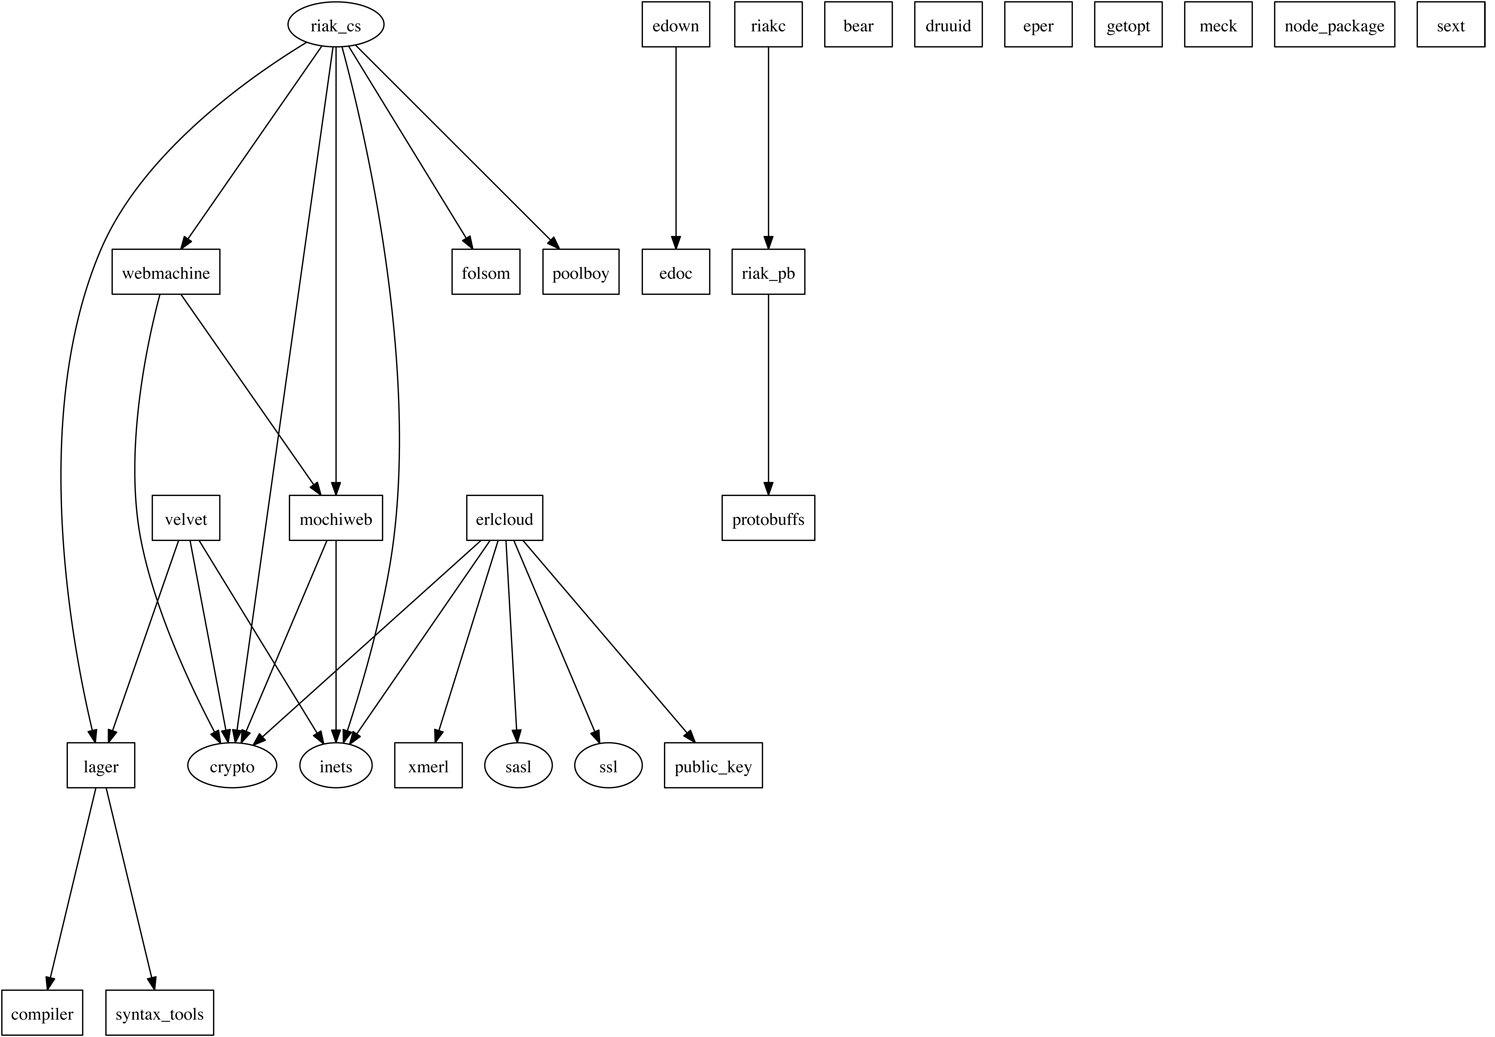
\includegraphics{app-deps-riak-cs.pdf}%
%  \caption{Dependency graph of riak\_cs, Basho's open source cloud library. The graph ignores dependencies on common applications like kernel and stdlib. Ovals are applications, rectangles are library applications.}%
  \caption{Граф зависимостей riak\_cs, облачной библиотеки с открытым исходным кодом, написанной компанией Basho. Граф игнорирует зависимости от общих приложений, таких как kernel и stdlib. Овалами показаны приложения, прямоугольниками --- библиотечные приложения.}%
   \label{fig:app-deps}
\end{figure}

%Using such a hierarchy and looking at each application's short description might be helpful to draw a rough, general map of where everything is located. To generate a similar diagram, find \app{recon}'s script directory and call \command{escript script/app\_deps.erl}\footnote{This script depends on graphviz}. Similar hierarchies can be found using the \module{observer}\footnote{\href{http://www.erlang.org/doc/apps/observer/observer\_ug.html}{http://www.erlang.org/doc/apps/observer/observer\_ug.html}} application, but for individual supervision trees. Put together, you may get an easy way to find out what does what in the code base.
Используя такую иерархию и глядя на короткое описание каждого из приложений, может оказаться полезным нарисовать приблизительную грубую карту где что находится. Для создания подобной диаграммы найдите в приложении \app{recon} директорию сценариев \filename{script/} и вызовите \command{escript script/app\_deps.erl}\footnote{Этот скрипт требует наличия у вас в системе программы graphviz}. Подобные иерархии можно найти используя \module{observer}\footnote{\href{http://www.erlang.org/doc/apps/observer/observer\_ug.html}{http://www.erlang.org/doc/apps/observer/observer\_ug.html}}, но для отдельных деревьев наблюдения. Если сложить это вместе, у вас может получиться удобный способ быстро нарисовать и разобраться, что происходит в незнакомом коде.


\FloatBarrier

\section{Ныряем в OTP-релизы}
\label{sec:dive-otp-releases}

%OTP releases are not a lot harder to understand than most OTP applications you'll encounter in the wild. A release is a set of OTP applications packaged in a production-ready manner so it boots and shuts down without needing to manually call \function{application:start/2} for any app. Of course there's a bit more to releases than that, but generally, the same discovery process used for individual OTP applications will be applicable here.
ОТР-релизы не сильно сложнее для понимания, чем обычные ОТР-приложения, которые могут вам встретиться в дикой природе. Релиз --- это набор ОТР-приложений, упакованных для доставки на производственные (\emph{production}) сервера так, что они запускаются и завершают работу без ручного вызова \function{application:start/2} в любом нужном вам приложении. Конечно есть и другие подробности касательно релизов, но обычно применяется тот же процесс исследования, как и для обычных приложений ОТР.

%You'll usually have a file similar to the configuration files used by \module{systools} or \module{reltool}, which will state all applications part of the release and a few\footnote{A lot} options regarding their packaging. To understand them, I recommend \href{http://learnyousomeerlang.com/release-is-the-word}{reading existing documentation on them}. If you're lucky, the project may be using \app{relx}\footnote{\href{https://github.com/erlware/relx/wiki}{https://github.com/erlware/relx/wiki}}, an easier tool that was officially released in early 2014.
Обычно у вас будет файл, похожий на файлы конфигурации, которыми пользуется  \module{systools} или \module{reltool}, который содержит перечень всех приложений, включённых в релиз и несколько\footnote{На самом деле множество.} параметров касательно способа их упаковки. Для лучшего их понимания я рекомендую обратиться к  \href{http://learnyousomeerlang.com/release-is-the-word}{чтению существующей документации и книгам}. Если вам повезло, проект мог быть собран с помощью \app{relx}\footnote{\href{https://github.com/erlware/relx/wiki}{https://github.com/erlware/relx/wiki}}, более удобного инструмента, который был официально выпущен в начале 2014.


\section{Упражнения}

\subsection*{\ReviewTitle{}}

\begin{enumerate}
%	\item How do you know if a code base is an application? A release?
	\item Как вы можете узнать, что данный код является приложением? Релизом?
%	\item What differentiates an application from a library application?
	\item Что отличает обычное приложение от библиотечного?
%	\item What can be said of processes under a \term{one\_for\_all} scheme for supervision?
	\item Что можно сказать о процессах, которые запускаются под наблюдателем по схеме \term{one\_for\_all}?
%	\item Why would someone use a \module{gen\_fsm} behaviour over a \module{gen\_server}?
	\item Почему кто-то может решить использовать поведение \module{gen\_fsm} вместо \module{gen\_server}?
\end{enumerate}

\subsection*{\HandsOnTitle{}}

%Download the code at \href{https://github.com/ferd/recon\_demo}{https://github.com/ferd/recon\_demo}. This will be used as a test bed for exercises throughout the book. Given you are not familiar with the code base yet, let's see if you can use the tips and tricks mentioned in this chapter to get an understanding of it.
Скачайте код отсюда: \href{https://github.com/ferd/recon\_demo}{https://github.com/ferd/recon\_demo}. Этот проект будет использоваться как основа для упражнений по всей книге. Подразумевается, что вы пока не знакомы с этим кодом, давайте посмотрим, как вы воспользуетесь знаниями, полученными в текущей главе и разберётесь что к чему.

\begin{enumerate}
%	\item Is this application meant to be used as a library? A standalone system?
	\item Задумано ли это приложение как библиотека или как отдельно работающая система?
%	\item What does it do?
	\item Что оно делает?
%	\item Does it have any dependencies? What are they?
	\item Есть ли у него зависимости? Какие?
%	\item The app's \filename{README} mentions being non-deterministic. Can you prove if this is true? How?
	\item Файл \filename{README} упоминает что-то о недетерминированности. Можете ли вы найти доказательства, что это правда? Как?
%	\item Can you express the dependency chain of applications in there? Generate a diagram of them?
	\item Можно ли здесь выразить цепочку зависимостей приложений? Создать диаграмму?
%	\item Can you add more processes to the main application than those described in the \filename{README}? 
	\item Можно ли добавить новые процессы к главному приложению кроме тех, что были описаны в файле \filename{README}?
\end{enumerate}
%%%
%%%
%%%

%%% Cognitive
%%
%% Knowledge: recall facts, terms, basic concepts
%% 
%% - How do you know if a code base is an application? A release?
%% - Where can you find what an application does?
%% - What differentiates an application from a library application?
%%
%% Comprehension: organizing, comparing, translating, interpreting, giving descriptions, and stating the main ideas
%%
%% - What can be said of processes under a one_for_all scheme for supervision?
%% - Why would someone use a gen_fsm process over a gen_server?
%%
%% Application: Solve problems in new situations by applying acquired knowledge, facts, techniques and rules in a different way
%%
%% Using the code at: https://github.com/ferd/recon_demo
%% - Is this application meant to be used as a library? A standalone system?
%% - What does it do?
%% - Does it have any dependencies? What are they?
%%
%% Analysis: break down info, make inferences, find evidence
%% - The app's readme mentions being non-deterministic. Can you prove if this is true? How?
%% - Can you express the dependency chain of applications in there? Generate a diagram of them?
%%
%% Synthesis: Compile information together in a different way by combining elements in a new pattern or proposing alternative solutions
%%
%% - Can you add more processes to the application? DO IT!
%%
%% Evaluation: Present and defend opinions by making judgments about information
%%
%% - Do you think the method you've chosen to add applications would work well operationally to be done live? If not, is this due to your choice or the application structure? 
%%

%%%
%%%
%%%

\chapter{Построение проектов с открытым исходным кодом на Erlang}
\label{chap:building-open-source-erlang-software}

%Most Erlang books tend to explain how to build Erlang/OTP applications, but few of them go very much in depth about how to integrate with the Erlang community doing Open Source work. Some of them even avoid the topic on purpose. This chapter dedicates itself to doing a quick tour of the state of affairs in Erlang.
Большинство книг по Erlang стараются объяснить, как построить приложения на Erlang/OTP, но совсем немногие углубляются в вопросы взаимодействия с сообществом, которое работает над приложениями с открытым исходным кодом (\emph{open source}). Некоторые даже специально избегают эту тему. Эта глава посвящена небольшой экскурсии по состоянию отношений между людьми и программами в Erlang.

%OTP applications are the vast majority of the open source code people will encounter. In fact, many people who would need to build an OTP release would do so as one umbrella OTP application. 
OTP-приложения являются подавляющим большинством исходных кодов, которые вы можете встретить. На самом деле многие люди, кому нужно собрать OTP-релиз, делают это в виде ещё одного приложения-зонтика, под которым размещаются все остальные части проекта.

%If what you're writing is a stand-alone piece of code that could be used by someone building a product, it's likely an OTP application. If what you're building is a product that stands on its own and should be deployed by users as-is (or with a little configuration), what you should be building is an OTP release.\footnote{The details of how to build an OTP application or release is left up to the Erlang introduction book you have at hand.}
Если то, что вы пишете, является отдельным набором файлов и кода, которые могут пригодиться кому-то ещё при построении их продукта, то вероятнее всего это будет оформлено, как приложение OTP.

%The main build tools supported are \app{rebar} and \app{erlang.mk}. The former is a portable Erlang script that will be used to wrap around a lot of standard functionality and add its own, while the latter is a very fancy makefile that does a bit less, but tends to be faster when it comes to compiling. In this chapter, I'll mostly focus on using \app{rebar} to build things, given it's the ad-hoc standard, is well-established, and \app{erlang.mk} applications tend to also be supported by \app{rebar} as dependencies.
Основные инструменты для сборки, которые получают поддержку авторов и сообщества --- это \app{rebar} и \app{erlang.mk}. Первое --- это портативный самодостаточный скрипт на языке Erlang, который является интерфейсом к ряду стандартных функций и добавляет некоторые свои, тогда как второе --- хитро закрученный стандартный сборочный файл (\emph{Makefile}), который делает немного меньше, но обычно выполняет компиляцию быстрее. В этой главе я в основном сосредоточусь на сборке с помощью \app{rebar}, поскольку он принят почти всеми, как стандарт, хорошо известен, а приложения, использующие \app{erlang.mk}, обычно поддерживаются при сборке с помощью \app{rebar} в качестве зависимостей.


\section{Структура проекта}
\label{sec:project-structure}

%The structures of OTP applications and of OTP releases are different. An OTP application can be expected to have one top-level supervisor (if any) and possibly a bunch of dependencies that sit below it. An OTP release will usually be composed of multiple OTP applications, which may or may not depend on each other. This will lead to two major ways to lay out applications.
Структуры приложений и релизов OTP отличаются. Ожидается, что OTP-приложение имеет один наблюдатель верхнего уровня (или ни одного) и, возможно, ряд зависимостей, которые находятся под ним. OTP-релиз обычно состоит из ряда ОТР-приложений, которые могут зависеть (или не зависеть) друг от друга. Это является причиной существования двух очень разных структур директорий.

\subsection{OTP-приложения}
\label{subsec:building-otp-applications}

%For OTP applications, the proper structure is pretty much the same as what was explained in \ref{sec:dive-otp-applications}:
Для ОТР-приложений правильной структурой является точно такая же, как мы рассмотрели ранее в секции \ref{sec:dive-otp-applications}:

\begin{VerbatimText}
doc/
deps/
ebin/
src/
test/
LICENSE.txt
README.md
rebar.config
\end{VerbatimText}

%What's new in this one is the \filename{deps/} directory, which is fairly useful to have, but that will be generated automatically by \app{rebar}\footnote{A lot of people package \app{rebar} directly in their application. This was initially done to help people who had never used rebar before use libraries and projects in a boostrapped manner. Feel free to install rebar globally on your system, or keep a local copy if you require a specific version to build your system.} if necessary. That's because there is no canonical package management in Erlang. People instead adopted \app{rebar}, which fetches dependencies locally, on a per-project basis. This is fine and removes a truckload of conflicts, but means that each project you have may have to download its own set of dependencies.
Какие появились отличия --- это директория \filename{deps/}, которую полезно иметь и она будет создана автоматически при работе с \app{rebar}\footnote{Многие люди пакуют \app{rebar} прямо в свои приложения. Изначально это помогало другим людям, которые никогда ранее им не пользовались, начать немедленно им пользоваться. На ваш вкус можно установить rebar глобально в вашей системе, или хранить локальную копию, если вам требуется особенная его версия.} по мере необходимости. Это происходит потому, что Erlang не имеет стандартного управления пакетами зависимостей. Вместо этого люди решили использовать \app{rebar}, который скачивает зависимости локально для каждого проекта свои. Это приемлемое решение и убирает массу проблем с конфликтами, но означает, что каждому проекту придётся скачивать свой набор зависимостей.

%This is accomplished with \app{rebar} by adding a few config lines to \filename{rebar.config}:
Зависимости для \app{rebar} задаются с помощью добавления строк в специальный файл \filename{rebar.config}, которого ваш проект может не иметь --- тогда создайте его сами:

\begin{VerbatimText}
{deps,
 [{application_name, "1.0.*",
   {git, "git://github.com/user/myapp.git", {branch,"master"}}},
  {application_name, "2.0.1",
   {git, "git://github.com/user/hisapp.git", {tag,"2.0.1"}}},
  {application_name, "", 
   {git, "https://bitbucket.org/user/herapp.git",  "7cd0aef4cd65"}},
  {application_name, "my regex",
   {hg, "https://bitbucket.org/user/theirapp.hg" {branch, "stable"}}}]}.
\end{VerbatimText}

%Applications are fetched directly from a \app{git} (or \app{hg}, or \app{svn}) source, recursively. They can then be compiled, and specific compile options can be added with the \expression{\{erl\_opts, List\}.} option in the config file\footnote{More details by calling \command{rebar help compile}}.
Приложения и их зависимости скачиваются рекурсивно с помощью стандартных утилит \app{git} (или \app{hg}, или \app{svn}) с указанных серверов. Затем они готовы к сборке и вы можете добавить особые параметры компиляции с помощью строки \expression{\{erl\_opts, СписокПараметров\}.} в файле конфигурации\footnote{Можно узнать подробнее, если выполнить \command{rebar help compile}}.

%Within these directories, you can do your regular development of an OTP application. To compile them, call \command{rebar get-deps compile}, which will download all dependencies, and then build them and your app at once.
В пределах этих директорий вы можете выполнять обычную разработку вашего ОТР-приложения. Для компиляции вызовите команду \command{rebar get-deps compile}, которая докачает недостающие зависимости и затем соберёт всё вместе с вашим приложением.

%When making your application public to the world, distribute it \emph{without} the dependencies. It's quite possible that other developers' applications depend on the same applications yours do, and it's no use shipping them all multiple times. The build system in place (in this case, \app{rebar}) should be able to figure out duplicated entries and fetch everything necessary only once.
Когда вы публикуете ваше приложение для всех желающих, то зависимости \emph{не включаются} в архив. Вполне возможна ситуация, когда приложения другого разработчика зависят от тех же приложений, что и ваше, и нет смысла поставлять ему наши копии зависимостей. Система сборки на компьютере другого разработчика (в нашем случае, \app{rebar}) сможет разобраться, какие зависимости нужны и докачает недостающие.

%% erlang.mk downloads relx for releases, and runs it iff there's a relx file there

\subsection{Строим OTP-релизы}
\label{subsec:building-otp-releases}

%For releases, the structure should be a bit different\footnote{I say \emph{should} because many Erlang developers put their final system under a single top-level application (in \filename{src}) and a bunch of follower ones as dependencies (in \filename{deps}), which is less than ideal for distribution purposes and conflicts with assumptions on directory structures made by OTP. People who do that tend to build from source on the production servers and run custom commands to boot their applications.}. Releases are collections of applications, and their structures should reflect that.
Для релизов структура должна немного отличаться\footnote{Я пишу \emph{должна} потому что многие Erlang-разработчики размещают свою готовую программу в единственном приложении на верхнем уровне проекта (в папке \filename{src/}) и ряд вспомогательных приложений оформляются, как зависимости (в папке \filename{deps/}), что не совсем идеально для нужд распространения программы и конфликтует с рекомендуемой стандартом ОТР структурой директорий. Люди, которые так делают, обычно собирают код из исходников при установке на производственные сервера и выполняют особые самодельные команды для их запуска.}. Релизы --- это наборы приложений, и их структура должна отражать этот факт.

%Instead of having a top-level app, applications should be nested one level deeper and divided into two categories: apps and deps. The apps directory contains your applications' source code (say, internal business code), and the deps directory contains independently managed dependency applications.
Вместо того, чтобы делать одно приложение верхнего уровня, следует разместить все приложения на один уровень глубже и разделить на две категории: собственно приложения (\emph{apps}) и зависимости (\emph{deps}). Директория \filename{apps/} содержит исходный код вашего приложения (скажем, ваша бизнес-логика), а директория \filename{deps/} содержит ваши зависимости, управляемые другими авторами или командами.

\begin{VerbatimRaw}
apps/
doc/
deps/
LICENSE.txt
README.md
rebar.config
\end{VerbatimRaw}

%This structure lends itself to generating releases. Tools such as Systool and Reltool have been covered before\footnote{\href{http://learnyousomeerlang.com/release-is-the-word}{http://learnyousomeerlang.com/release-is-the-word}}, and can allow the user plenty of power. An easier tool that recently appeared is \app{relx}\footnote{\href{https://github.com/erlware/relx/wiki}{https://github.com/erlware/relx/wiki}}.
Эта структура годится для генерации релизов. Инструменты, такие как Systool и Reltool были описаны в других публикациях\footnote{\href{http://learnyousomeerlang.com/release-is-the-word}{http://learnyousomeerlang.com/release-is-the-word}}, и могут дать пользователю большую власть. Более лёгкий инструмент, который появился совсем недавно --- это \app{relx}\footnote{\href{https://github.com/erlware/relx/wiki}{https://github.com/erlware/relx/wiki}}.

%A  \app{relx} configuration file for the directory structure above would look like:
Файл конфигурации для \app{relx}, описывающий структуру директорий, показанную выше, будет выглядеть так:

\begin{VerbatimText}
{paths, ["apps", "deps"]}.
{include_erts, false}. % релиз будет использовать установленный в системе Erlang
{default_release, demo, "1.0.0"}.

{release, {demo, "1.0.0"},
    [members,
     feedstore,
     ...
     recon]}.
\end{VerbatimText}

%Calling \command{./relx} (if the executable is in the current directory) will build a release, to be found in the \filename{\_rel/} directory. If you really like using \app{rebar}, you can build a release as part of the project's compilation by using a rebar hook in \filename{rebar.config}:
Вызов команды \command{./relx} (если исполняемый файл relx находится в текущей директории) начнёт сборку релиза, который будет помещён в директорию \filename{\_rel/}. Если вам нравится пользоваться программой \app{rebar}, то вы можете построить релиз в процессе компиляции проекта используя такую строчку в \filename{rebar.config}:

\begin{VerbatimText}
{post_hooks,[{compile, "./relx"}]}.
\end{VerbatimText}

%And every time \command{rebar compile} will be called, the release will be generated.
Тогда каждый раз, когда вы вызовете команду \command{rebar compile}, будет создаваться релиз.

\section{Наблюдатели и семантика start\_link}
\label{sec:supervisors-and-start-link-semantics}

%In complex production systems, most faults and errors are transient, and retrying an operation is a good way to do things — Jim Gray's paper\footnote{\href{http://mononcqc.tumblr.com/post/35165909365/why-do-computers-stop}{http://mononcqc.tumblr.com/post/35165909365/why-do-computers-stop}} quotes \emph{Mean Times Between Failures} (MTBF) of systems handling transient bugs being better by a factor of 4 when doing this. Still, supervisors aren't just about restarting.
В сложной производственной (\emph{production}) системе многие сбои и ошибки являются временными, и повторная попытка выполнить операцию --- это хороший подход к ведению дел, согласно работе Джима Грэй \footnote{\href{http://mononcqc.tumblr.com/post/35165909365/why-do-computers-stop}{http://mononcqc.tumblr.com/post/35165909365/why-do-computers-stop}}, которая цитирует, что \emph{среднее время наработки до отказа} (\emph{Mean Times Between Failures или сокращённо MTBF}) систем, которые обрабатывают такие временные ошибки, улучшается в 4 раза. И всё же тема наблюдателей затрагивает больше, чем просто перезапуски.

%One very important part of Erlang supervisors and their supervision trees is that \emph{their start phases are synchronous}. Each OTP process has the potential to prevent its siblings and cousins from booting. If the process dies, it's retried again, and again, until it works, or fails too often.
Одним из важных фактов о наблюдателях в Erlang и их деревьях наблюдения является то, что \emph{фазы их запуска синхронны}. Каждый процесс в OTP имеет возможность заблокировать запуск своих дочерних и сестринских процессов. Если процесс завершается аварийно (умирает), то попытка повторяется снова и снова, пока он не запустится успешно или наблюдатель не сочтёт, что процесс падает слишком часто.

%That's where people make a very common mistake. There isn't a backoff or cooldown period before a supervisor restarts a crashed child. When a network-based application tries to set up a connection during its initialization phase and the remote service is down, the application fails to boot after too many fruitless restarts. Then the system may shut down.
Здесь люди часто делают одну общую ошибку. Нет никакой паузы перед тем, как наблюдатель перезапускает упавший дочерний процесс. Когда сетевое приложение пытается установить подключение во время фазы своей инициализации в то время, как удалённый сервис не работает, приложение не может загрузиться после ряда безуспешных перезапусков. Затем система останавливается целиком.

%Many Erlang developers end up arguing in favor of a supervisor that has a cooldown period. I strongly oppose the sentiment for one simple reason: \emph{it's all about the guarantees}.
Много Erlang-разработчиков скатываются в споры о создании наблюдателя, который бы имел период ожидания между перезапусками. Я выступаю против этой идеи по одной простой причине: \emph{дело в том, какие вы получаете гарантии}.

\subsection{Всё дело в гарантии}
\label{subsec:start-link-guarantees}

%Restarting a process is about bringing it back to a stable, known state. From there, things can be retried. When the initialization isn't stable, supervision is worth very little. An initialized process should be stable no matter what happens. That way, when its siblings and cousins get started later on, they can be booted fully knowing that the rest of the system that came up before them is healthy.
Перезапуск процесса --- это перевод его в стабильное и заранее известное состояние. С этого момента можно повторно выполнять какие-то неудачные операции. Если инициализация нестабильна, то наблюдение за процессом не стоит и гроша. Инициализированный начисто процесс должен быть стабильным что бы ни произошло. Таким образом, когда дочерние и сестринские процессы перезапустятся в будущем, они будут уверены в том, что остальная система, запущенная до них, в хорошем состоянии и исправна.

%If you don't provide that stable state, or if you were to start the entire system asynchronously, you would get very little benefit from this structure that a \expression{try ... catch} in a loop wouldn't provide.
Если вы не обеспечите такое стабильное состояние, или если вы запускаете всю систему асинхронно, то такая структура даст вам мало преимуществ по сравнению с запуском \expression{try} ... \expression{catch} в цикле.

%Supervised processes \emph{provide guarantees} in their initialization phase, \emph{not a best effort}. This means that when you're writing a client for a database or service, you shouldn't need a connection to be established as part of the initialization phase unless you're ready to say it will always be available no matter what happens.
Процессы под наблюдением \emph{обеспечивают гарантии} в фазе их инициализации, в отличие от \emph{попыток сделать всё возможное}. Это означает, что когда вы пишете клиент для базы данных или сервис, вам не потребуется проверять наличие подключения в ходе фазы инициализации, если вы можете утверждать, что оно всегда будет доступно вне зависимости от ситуации.

%You could force a connection during initialization if you know the database is on the same host and should be booted before your Erlang system, for example. Then a restart should work. In case of something incomprehensible and unexpected that breaks these guarantees, the node will end up crashing, which is desirable: a pre-condition to starting your system hasn't been met. It's a system-wide assertion that failed.
Например вы могли бы принудительно выполнить подключение во время инициализации, если вы знаете, что база данных находится на одном с вами сервере и должна запуститься до старта вашей Erlang-системы. Тогда перезапуск сработал бы. В случае, если случится нечто непонятное и неожиданное, нарушающее эти гарантии, то ваш узел завершит работу аварийно, что вполне нам подходит: предварительное условие для запуска системы не было выполнено. Обязательная для старта системы тестовая проверка не прошла.

%If, on the other hand, your database is on a remote host, you should expect the connection to fail. It's just a reality of distributed systems that things go down.\footnote{Or latency shoots up enough that it is impossible to tell the difference from failure.} In this case, the only guarantee you can make in the client process is that your client will be able to handle requests, but not that it will communicate to the database. It could return \expression{\{error, not\_connected\}} on all calls during a net split, for example.
Если же, с другой стороны, ваша база данных находится на удалённом сервере, то следует быть готовыми к тому, что подключение завершится неудачей. Это повседневная реальность распределённых систем --- их части постоянно отказывают\footnote{Или сетевая задержка увеличивается настолько, что становится трудно отличить ситуацию от полного отказа.}. В таком случае единственной гарантией, которую вы можете обеспечить в клиенстком процессе будет то, что ваш клиент сможет обработать запросы, но не подключиться к базе данных. Например, он мог бы возвращать \expression{\{error,} \expression{not\_connected\}} на все вызовы во время разделения сети.

%The reconnection to the database can then be done using whatever cooldown or backoff strategy you believe is optimal, without impacting the stability of the system. It can be attempted in the initialization phase as an optimization, but the process should be able to reconnect later on if anything ever disconnects.
Повторное подключение к базе данных затем может произойти с любой удобной вам частотой или задержкой, не влияя на стабильность работы системы. Попытка также может быть выполненя в фазе инициализации, в качестве оптимизации, но процесс должен уметь повторно подключиться позже в случае отказа или отключения.

%If you expect failure to happen on an external service, do not make its presence a guarantee of your system. We're dealing with the real world here, and failure of external dependencies is always an option. 
Если вы ожидаете, что внешний сервис откажет, не делайте его наличие обязательной гарантией для вашей системы. Мы здесь работаем с реальным миром, и отказ внешних зависимостей может произойти в любой момент.


\subsection{Побочные эффекты}
\label{subsec:start-link-side-effects}

%Of course, the libraries and processes that call such a client will then error out if they don't expect to work without a database. That's an entirely different issue in a different problem space, one that depends on your business rules and what you can or can't do to a client, but one that is possible to work around. For example, consider a client for a service that stores operational metrics — the code that calls that client could very well ignore the errors without adverse effects to the system as a whole. 
Само собой, библиотеки и процессы, которые используют такой клиент, могут вылететь с ошибкой, если они не ожидают неожиданно оказаться без базы данных. Эта проблема совсем иная и лежит в другой плоскости, которая зависит от правил вашей бизнес-логики и того, что вы можете или не можете делать с клиентом, но проблема вполне решаемая. Например, представьте себе клиент некоторого сервиса, хранящий операционные метрики --- код, который вызывает этого клиента, может игнорировать ошибки и они не окажут ощутимого влияния на работу системы в целом.

%The difference in both initialization and supervision approaches is that the client's callers make the decision about how much failure they can tolerate, not the client itself. That's a very important distinction when it comes to designing fault-tolerant systems. Yes, supervisors are about restarts, but they should be about restarts to a stable known state.
Разница в подходах к инициализации и наблюдению за процессами в том, что не наш клиент, а вызывающие его процессы принимают решение о том, насколько они готовы терпеть сбои и ошибки. Это очень важное различие, когда дело касается проектирования устойчивых к сбоям систем. Да, наблюдатели только и делают, что занимаются перезапусками, но суть в том, что перезапуски должны приводить к стабильному и известному заранее состоянию.


%\subsection{Example: Initializing without guaranteeing connections}
\subsection{Пример: Инициализация без гарантии подключения}
\label{subsec:start-link-initializing-without-guaranteeing-connections}

%The following code attempts to guarantee a connection as part of the process' state:
Следующий код пытается гарантировать наличие живого соединения при запуске процесса:

\begin{VerbatimText}
init(Args) ->
    Opts = parse_args(Args),
    {ok, Port} = connect(Opts),
    {ok, #state{sock=Port, opts=Opts}}.

[...]

handle_info(reconnect, S = #state{sock=undefined, opts=Opts}) ->
    %% попытаемся подключиться в цикле
    case connect(Opts) of
        {ok, New} -> {noreply, S#state{sock=New}};
         _ -> self() ! reconnect, {noreply, S}
    end;
\end{VerbatimText}

%Instead, consider rewriting it as:
Вместо этого попробуйте переписать его так:

\begin{VerbatimText}
init(Args) ->
    Opts = parse_args(Args),
    %% вы всё равно можете попытаться подключиться прямо здесь, чтобы по 
    %% возможности улучшить доступность, но будьте готовы, что подключение 
    %% не удастся
    self() ! reconnect,
    {ok, #state{sock=undefined, opts=Opts}}.

[...]

handle_info(reconnect, S = #state{sock=undefined, opts=Opts}) ->
    %% попытаемся подключиться в цикле
    case connect(Opts) of
        {ok, New} -> {noreply, S#state{sock=New}};
        _ -> self() ! reconnect, {noreply, S}
    end;
\end{VerbatimText}

%You now allow initializations with fewer guarantees: they went from \emph{the connection is available} to \emph{the connection manager is available}.
\sloppy{}
Теперь вы можете позволить инициализацию с меньшим количеством гарантий: раньше требовалась гарантия \emph{наличия подключения}, а сейчас требуется просто \emph{наличие менеджера подключений}.


\subsection{В двух словах}
\label{subsec:start-link-in-a-nutshell}

%Production systems I have worked with have been a mix of both approaches.
Производственные (\emph{production}) системы, с которыми мне довелось работать, использовали и тот и другой подход.

%Things like configuration files, access to the file system (say for logging purposes), local resources that can be depended on (opening UDP ports for logs), restoring a stable state from disk or network, and so on, are things I'll put into requirements of a supervisor and may decide to synchronously load no matter how long it takes (some applications may just end up having over 10 minute boot times in rare cases, but that's okay because we're possibly syncing gigabytes that we \emph{need} to work with as a base state if we don't want to serve incorrect information.)
Такие вещи, как файлы конфигурации, доступ к файловой системе (например, для потребностей ведения файлов журналов), локальные ресурсы, от которых могла бы зависеть система (открытие UDP-портов для ведения журналов), восстановление стабильного состояния из диска или по сети и так далее. Это те вещи, которые я помещаю в требования к наблюдателю и могу решить загрузить их синхронно независимо от того, сколько бы это ни потребовало времени (некоторые приложения иногда могут требовать более десяти минут для запуска, но это приемлемо, поскольку мы в этот момент перелопачиваем гигабайты, которые нам \emph{нужны} для работы в качестве базового состояния, если мы не хотим отдавать клиентам некорректные или неполные ответы).

%On the other hand, code that depends on non-local databases and external services will adopt partial startups with quicker supervision tree booting because if the failure is expected to happen often during regular operations, 
%then there's no difference between now and later. You have to handle it the same, and for these parts of the system, far less strict guarantees are often the better solution.
С другой стороны код, который зависит от удалённых баз данных и внешних сервисов, будет использовать запуск с частичными подключениями для ускорения запуска деревьев наблюдения, поскольку сбои ожидаются достаточно часто во время обычной работы, то и нет разницы в том, случится ли сбой при запуске или позже. Ваш подход к обработке этих ситуаций будет одинаковым, и для этих частей системы намного лучшим решением будет уменьшение гарантий.


%Application Strategies
\subsection{Стратегии приложений}
\label{subsec:start-link-application-strategies}

%No matter what, a sequence of failures is not a death sentence for the node. Once a system has been divided into various OTP applications, it becomes possible to choose which applications are vital or not to the node. Each OTP application can be started in 3 ways: temporary, transient, permanent, either by doing it manually in \expression{application:start(Name, Type)}, or in the config file for your release:
\sloppy{}
Вне зависимости от того, что произошло, ряд отказов не является смертельным приговором для узла. Как только система разделена на различные ОТР-приложения, становится возможным выбирать, какие из приложений являются жизненно-важными для узла. Каждое из приложений в ОТР может запускаться в трёх режимах: как временное (\emph{temporary}), преходящее или недолговечное (\emph{transient}) или постоянное (\emph{permanent}). Это делается либо вручную, выполняя команду \expression{application:start(Имя, Тип)}, либо из файла конфигурации вашего релиза:

\begin{itemize*}
%	\item \term{permanent}: if the app terminates, the entire system is taken down, excluding manual termination of the app with \function{application:stop/1}.
	\item Постоянное (\term{permanent}): если приложение завершит работу, то вся система останавливается, кроме тех случаев, когда приложение было остановлено вручную командой \function{application:stop/1}.
%	\item \term{transient}: if the app terminates for reason \term{normal}, that's ok. Any other reason for termination shuts down the entire system.
	\item Преходящее (\term{transient}): если приложение завершится по причине \term{normal}, то всё в порядке. Любая другая причина завершения работы останавливает всю систему.
%	\item \term{temporary}: the application is allowed to stop for any reason. It will be reported, but nothing bad will happen.
	\item Временное (\term{temporary}): приложению разрешено останавливаться нормально и аварийно, по любой причине. О ситуации будет доложено в журналы или на экран, но ничего плохого больше не произойдёт.
\end{itemize*}

%It is also possible to start an application as an \emph{included application}, which starts it under your own OTP supervisor with its own strategy to restart it.
Также возможно запустить приложение в качестве \emph{вложенного приложения} (\emph{included application}), что запустит его под наблюдателем ОТР со своей собственной стратегией перезапуска.


\section{Упражнения}

\subsection*{\ReviewTitle}

\begin{enumerate}
%	\item  Are Erlang supervision trees started depth-first? breadth-first? Synchronously or asynchronously?
	\item Запускаются ли деревья наблюдения в Erlang в глубину или в ширину? Синхронно или асинхронно?
%	\item What are the three application strategies? What do they do?
	\item Какие бывают три стратегии приложений? Что они делают?
%	\item What are the main differences between the directory structure of an app and a release?
	\item Какие главные различия между структурами директорий приложения и релиза?
%	\item When should you use a release?
	\item Когда следует использовать релиз?
%	\item Give two examples of the type of state that can go in a process' init function, and two examples of the type of state that shouldn't go in a process' init function
	\item Дайте два примера состояний, которые могут быть помещены в функцию инициализации процесса и два примера состояний, которые не следует туда помещать.
\end{enumerate}

\subsection*{\HandsOnTitle{}}

%Using the code at
Используйте код, который находится по адресу
\href{https://github.com/ferd/recon\_demo}{https://github.com/ferd/recon\_demo}:

\begin{enumerate}
%	\item Extract the main application hosted in the release to make it independent, and includable in other projects.
	\item Извлеките главное приложение, которое хранится в релизе, и сделайте его независимым с возможностью включения в другие проекты.
%	\item Host the application somewhere (Github, Bitbucket, local server), and build a release with that application as a dependency.
	\item Разместите приложение где-нибудь (Github, Bitbucket или ваш собственный сервер) и соберите релиз с этим приложением в качестве зависимости.
%	\item The main application's workers (\module{council\_member}) starts a server and connects to it in its \function{init/1} function. Can you make this connection happen outside of the init function's? Is there a benefit to doing so in this specific case?
	\item Рабочий процесс главного приложения (\module{council\_member}) запускает сервер и подключается к нему в своей функции \function{init/1}. Можно ли сделать это подключение за пределами функции init? Есть ли выгода от этого в данном конкретном случае?
\end{enumerate}

%%
%% Knowledge: recall facts, terms, basic concepts
%% 
%% - Does Erlang have package management? Where do dependencies live in a system?
%% - What are the commands to build an Erlang project using rebar?
%% - What tools are available to build releases?
%% - Are Erlang supervision trees started depth-first? breadth-first? Synchronously or asynchronously?
%% - What are the three application strategies?
%%
%% Comprehension: organizing, comparing, translating, interpreting, giving descriptions, and stating the main ideas
%%
%% - What are the main differences between the directory structure of an app? of a release?
%% - When should you use a release?
%%
%% Application: Solve problems in new situations by applying acquired knowledge, facts, techniques and rules in a different way
%%
%% Using the code at: https://github.com/ferd/recon_demo
%% - Extract the main application hosted in the release to make it independent, and includable in other projects
%% - Build a release with the app that was turned as a dependency
%%
%% Analysis: break down info, make inferences, find evidence
%% - Give two examples of the type of state that can go in a process' init function
%% - Give two examples of the type of state that should not go in a process' init function
%%
%% Synthesis: Compile information together in a different way by combining elements in a new pattern or proposing alternative solutions
%%
%% - Give example of applications you would design as temporary, transient, and permanent
%%
%% Evaluation: Present and defend opinions by making judgments about information
%%
%% - Do you think OTP supervisors should offer a back-off strategy on restart?
%% - What are the build tools you would choose for your app?
%%

%%%
%%%
%%%

%Planning for Overload
\chapter{В ожидании перегрузки}
\label{chap:overload}

%By far, the most common cause of failure I've encountered in real-world scenarios is due to the node running out of memory. Furthermore, it is usually related to message queues going out of bounds.\footnote{Figuring out that a message queue is the problem is explained in Chapter \ref{chap:crash-dumps}, specifically in Section \ref{sec:crash-full-mailboxes}} There are plenty of ways to deal with this, but knowing which one to use will require a decent understanding of the system you're working on.
Без сомнения одной из самых частых причин сбоев, которые мне встречались в ситуациях реального мира, это переполнение памяти на узлах. Более того, обычно это связано с очередями сообщений, которые растут бесконтрольно\footnote{Как разобраться, что именно очередь сообщений оказалась проблемой, объясняется в Главе \ref{chap:crash-dumps}, а именно в Секции \ref{sec:crash-full-mailboxes}}. Есть множество способов справиться с этой бедой, но выбор правильного решения потребует хорошего понимания системы, с которой вам довелось работать.

%To oversimplify things, most of the projects I end up working on can be visualized as a very large bathroom sink. User and data input are flowing from the faucet. The Erlang system itself is the sink and the pipes, and wherever the output goes (whether it's a database, an external API or service, and so on) is the sewer system.
Если говорить упрощённо, то большинство проектов, с которыми мне пришлось работать, могут быть изображены в виде кухонной раковины. Пользовательские и входящие данные вытекают из крана. Erlang-система является раковиной и трубами, а то, куда идёт вывод результатов (неважно, что это, база данных или внешний сервис) --- является канализацией.

\begin{figure}[h!]
  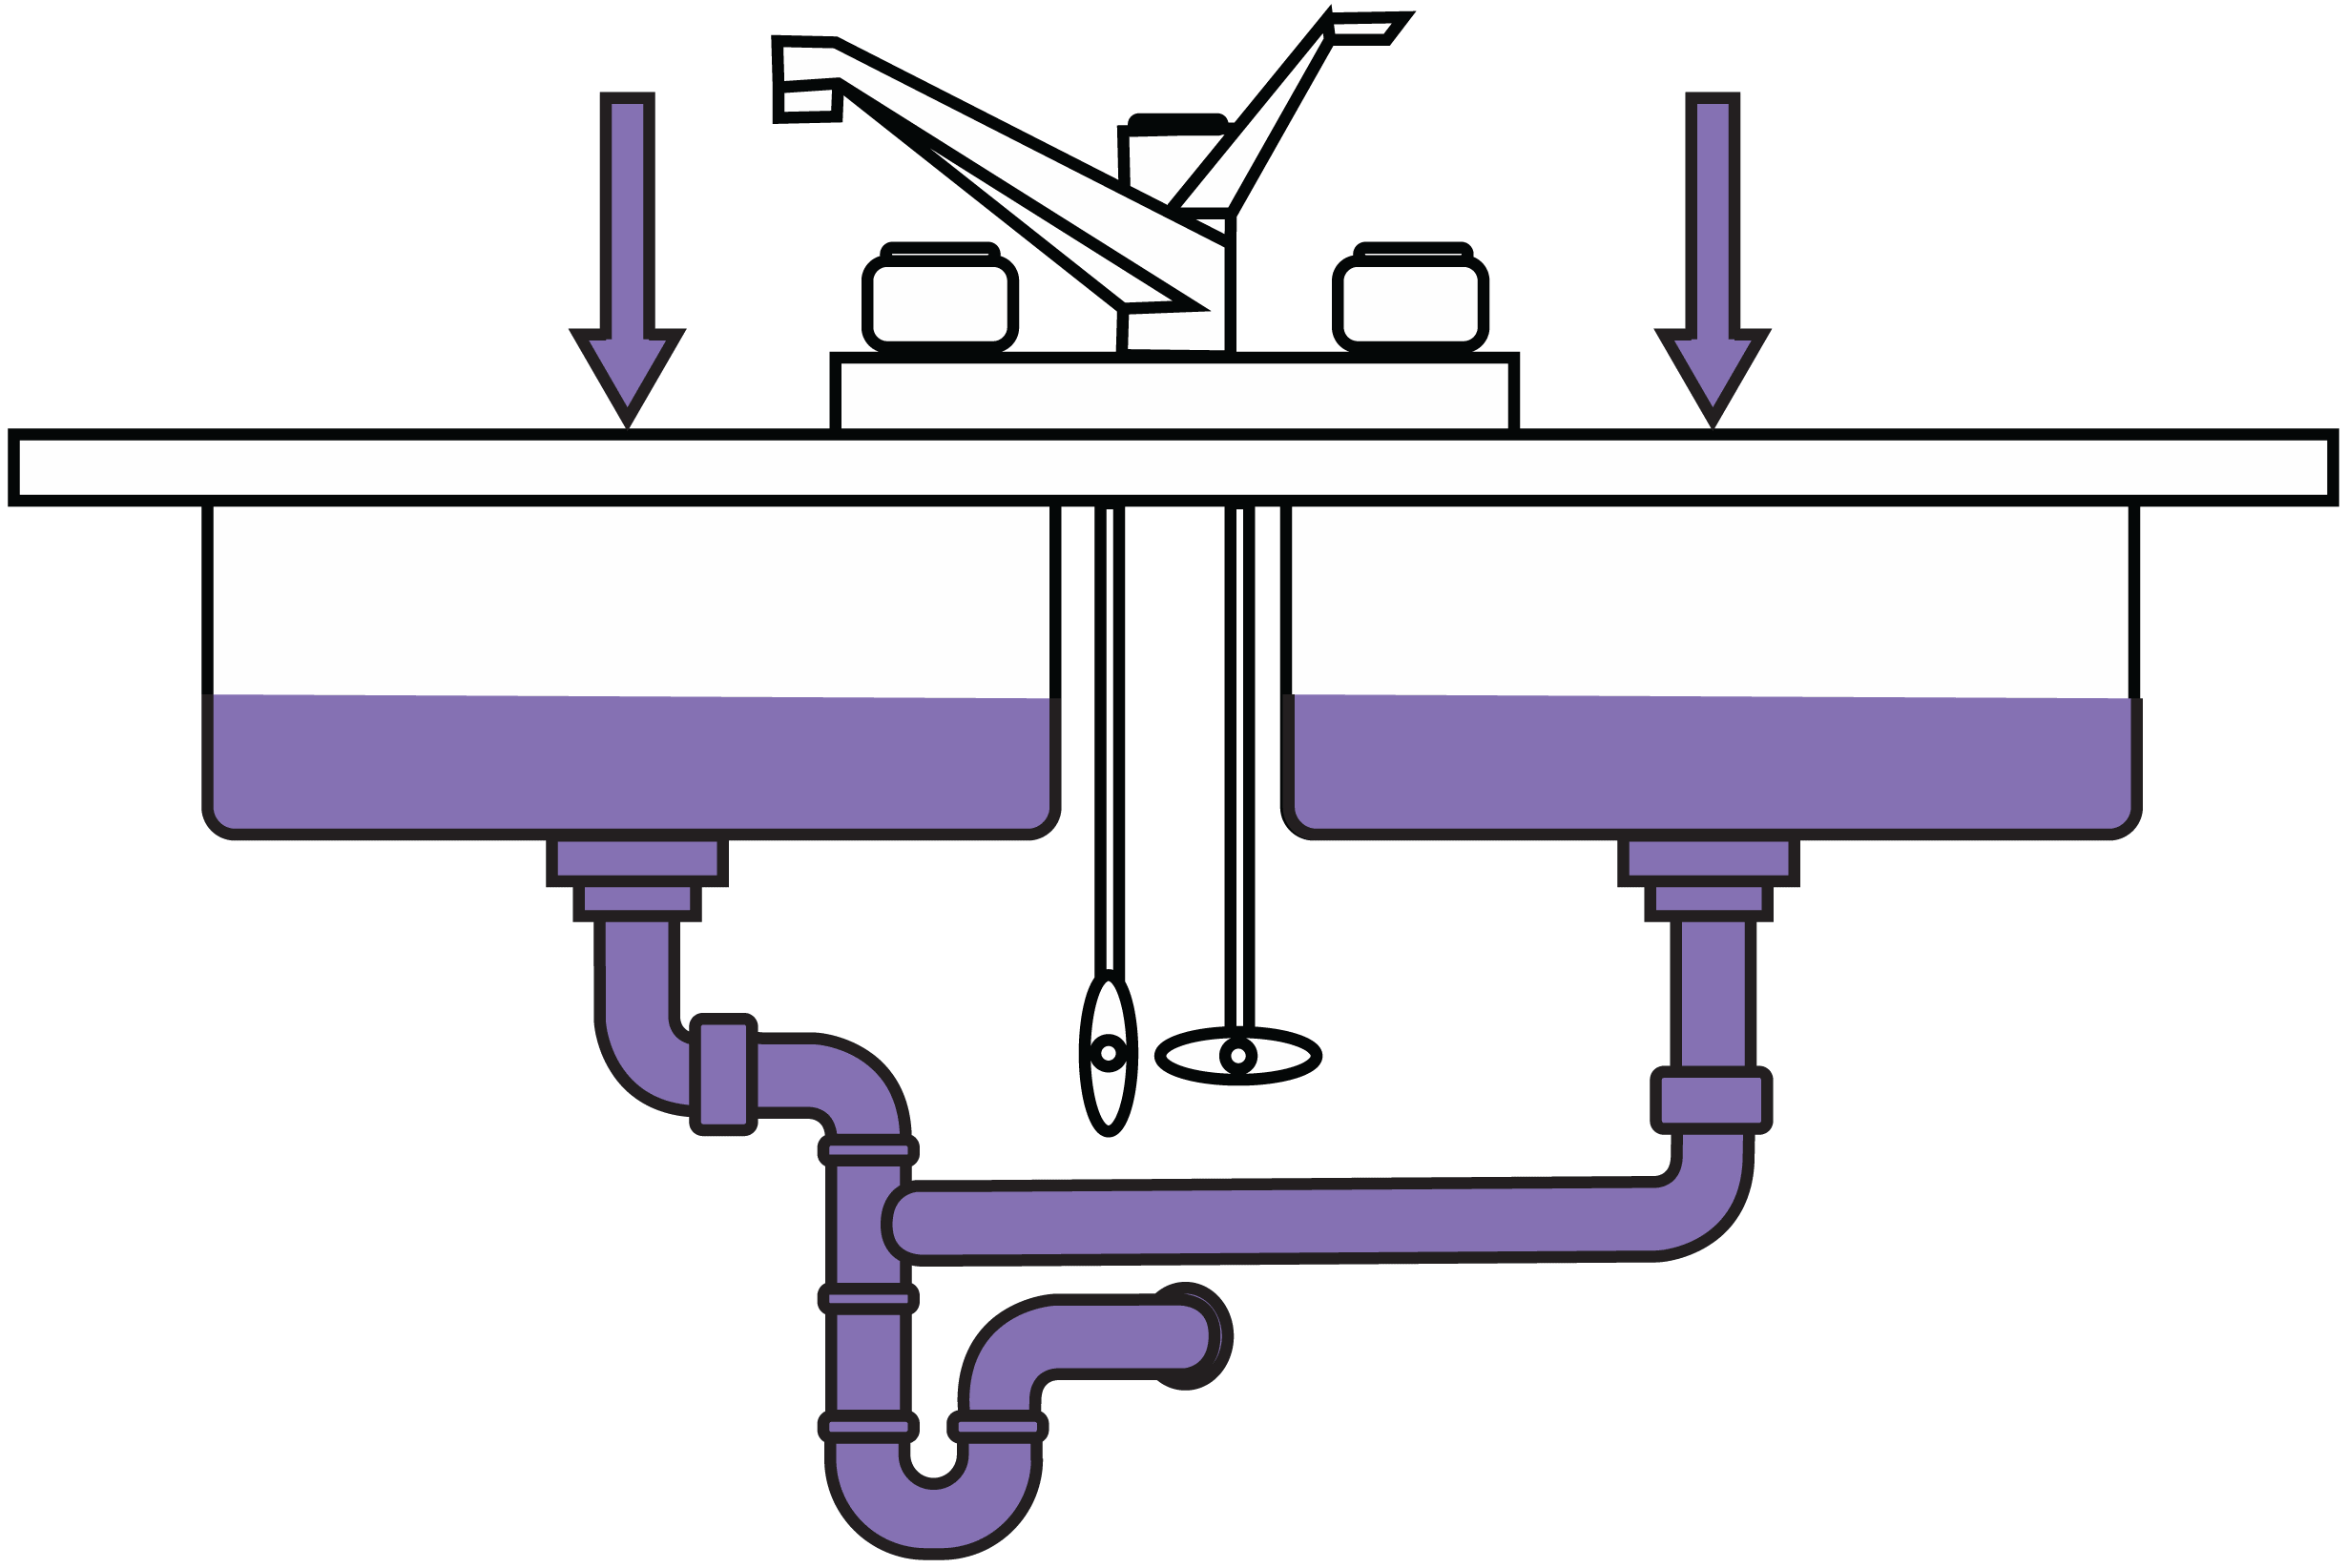
\includegraphics[max height=7cm]{sink.pdf}%
  \centering%
%  \caption{Your system is like a sink, and the true bottleneck, at the last drain, needs to be identified before you spend all your time and money making the sink and pipes bigger.}%
%\caption{Ваша система в виде раковины, и настоящее узкое место в последней трубе должно быть обнаружено до того, как вы потратите слишком много времени и денег увеличивая трубы и раковину.}
   \label{fig:tracing-venn}
\end{figure}

%When an Erlang node dies because of a queue overflowing, figuring out who to blame is crucial. Did someone put too much water in the sink? Are the sewer systems backing up? Did you just design too small a pipe?
Когда узел Erlang умирает по причине переполнения очереди, очень важно найти виновного. Вдруг налили слишком много воды? Справляется ли канализация? Не занизили ли вы размеры труб в проекте?

%Determining what queue blew up is not necessarily hard. This is information that can be found in a crash dump. Finding out why it blew up is trickier. Based on the role of the process or run-time inspection, it's possible to figure out whether causes include fast flooding, blocked processes that won't process messages fast enough, and so on.
Определить, какая из очередей взлетела на воздух будет нетрудно. Эту информацию можно обнаружить в файле дампа после смерти узла. А вот поиск причины, по которой это произошло --- более хитрая задача. Основываясь на роли процесса или изучении ситуации во время работы системы, можно вычислить причины --- произошёл ли резкий всплеск числа сообщений, заблокированные процессы, которые не успевали выбирать сообщения, и так далее.

%The most difficult part is to decide how to fix it. When the sink gets clogged up by too much waste, we will usually start by trying to make the bathroom sink itself larger (the part of our program that crashed, at the edge). Then we figure out the sink's drain is too small, and optimize that. Then we find out the pipes themselves are too narrow, and optimize that. The overload gets pushed further down the system, until the sewers can't take it anymore. At that point, we may try to add sinks or add bathrooms to help with the global input level.
Самой трудной частью будет принятие решения о способе починки. Когда раковина заполняется отходами, мы обычно пытаемся увеличить размеры раковины (та часть программы, которая упала, первое, что мы видим). Затем мы догадываемся, что сток слишком мал и пытаемся улучшить этот момент. Затем обнаруживается, что трубы слишком узкие, и решаем эту проблему. Перегрузка оттесняется вглубь системы до тех пор, пока канализация не отказывается увеличивать принятые объёмы. В этот момент мы можем решить добавить больше раковин или увеличить число ванных комнат для решения проблемы с входными данными.

%Then there's a point where things can't be improved anymore at the bathroom's level. There are too many logs sent around, there's a bottleneck on databases that \emph{need} the consistency, or there's simply not enough knowledge or manpower in your organization to improve things there.
Затем наступает момент, когда на уровне ванной комнаты мы больше ничего не можем улучшить. Слишком много событий отправляется в журналы сообщений, или база данных с обязательным \emph{требованием целостности} оказалась узким местом, или в нашей компании просто не хватает людей или ума, чтобы улучшить что-нибудь ещё.

%By finding that point, we identified what the \emph{true bottleneck} of the system was, and all the prior optimization was nice (and likely expensive), but it was more or less in vain.
Когда мы находим эту границу, можно считать, что \emph{истинное узкое место} системы было обнаружено, и вся предыдущая оптимизация была полезной (и, наверное, дорогой), но всё было сделано зря.

%We need to be more clever, and so things are moved back up a level. We try to massage the information going in the system to make it either lighter (whether it is through compression, better algorithms and data representation, caching, and so on). 
Нам нужно быть умнее, и перенести наше внимание на уровень выше. Мы попытаемся заняться информацией, входящей в систему, и сделать её легче (с помощью сжатия, улучшения алгоритмов или представления данных, кэширования и так далее).

%Even then, there are times where the overload will be too much, and we have to make the hard decisions between restricting the input to the system, discarding it, or accepting that the system will reduce its quality of service up to the point it will crash. These mechanisms fall into two broad strategies: back-pressure and load-shedding.
Бывают моменты, когда перегрузка слишком сильная, и нам приходится принимать трудный выбор между ограничением ввода в систему, уничтожением части входящих данных или смириться с фактом, что система понизит качество обслуживания вплоть до полной аварийной остановки. Эти механизмы можно объединить в две широкие категории: обратное давление (\emph{back-pressure}) и сброс лишней нагрузки (\emph{load-shedding}).

%We'll explore them in this chapter, along with common events that end up causing Erlang systems to blow up.
Мы рассмотрим их в этой главе вместе с общими событиями, которые могут привести к тому, что Erlang-системы взлетают на воздух.


%\section{Common Overload Sources}
\section{Обычные источники перегрузок}

%There are a few common causes of queues blowing up and overload in Erlang systems that most people will encounter sooner or later, no matter how they approach their system. They're usually symptomatic of having your system grow up and require some help scaling up, or of an unexpected type of failure that ends up cascading much harder than it should have.
Есть несколько известных причин того, что размеры очередей сообщений в Erlang-системах выходят из-под контроля, и рано или поздно многие люди с этими ситуациями сталкиваются независимо от их подхода к работе с системой. Обычно эти причины симптоматично проявляются в виде необходимости роста системы и требуют некоторой помощи для облегчения масштабирования, или в виде неожиданного сбоя, который в результате каскадно распространяется и приводит к более тяжёлым последствиям, чем следовало бы.

%\subsection{error\_logger Explodes}
\subsection{Взрыв в error\_logger}

%Ironically, the process in charge of error logging is one of the most fragile ones. In a default Erlang install, the \module{error\_logger}\footnote{Defined at \href{http://www.erlang.org/doc/man/error\_logger.html}{http://www.erlang.org/doc/man/error\_logger.html}} process will take its sweet time to log things to disk or over the network, and will do so much more slowly than errors can be generated.
По странной иронии, процесс, отвечающий за журналирование ошибок одновременно является одним из самых хрупких. В установленном по умолчанию Erlang, процесс \module{error\_logger}\footnote{Описан здесь: \href{http://www.erlang.org/doc/man/error\_logger.html}{http://www.erlang.org/doc/man/error\_logger.html}} не торопясь журналирует события на диск или по сети, и часто делает это медленнее, чем появляются новые ошибки.

%This is especially true of user-generated log messages (not for errors), and for crashes in large processes. For the former, this is because \module{error\_logger} doesn't really expect arbitrary levels of messages coming in continually. It's for exceptional cases only and doesn't expect lots of traffic. For the latter, it's because the entire state of processes (including their mailboxes) gets copied over to be logged. It only takes a few messages to cause memory to bubble up a lot, and if that's not enough to cause the node to run Out Of Memory (OOM), it may slow the logger enough that additional messages will.
Это в особенности верно для пользовательских сообщений (не для ошибок), и для аварийного завершения особо больших процессов. Для первого это является проблемой потому, что \module{error\_logger} просто не готов к приёму произвольных сообщений, которые идут постоянным потоком. Он предназначен для исключительных ситуаций и не ожидает большого движения данных. А второе потому, что всё состояние процесса целиком копируется для записи в журнал (включая содержимое его почтового ящика). Всего лишь несколько таких сообщений и потребление памяти вспучивается пузырём, и даже если это не обрушивает весь узел по перерасходу памяти (\emph{out of memory или OOM}), то однозначно замедлит процесс журналирования настолько, что дополнительные сообщения его добьют.

%The best solution for this at the time of writing is to use \href{https://github.com/basho/lager}{\otpapp{lager}} as a substitute logging library.
Лучшим решением в таком случае (на момент написания этого текста) будет замена библиотеки журналирования на \href{https://github.com/basho/lager}{\otpapp{lager}}.

%While \otpapp{lager} will not solve all your problems, it will truncate voluminous log messages, optionally drop OTP-generated error messages when they go over a certain threshold, and will automatically switch between asynchronous and synchronous modes for user-submitted messages in order to self-regulate.
В то время как \otpapp{lager} не решит всех ваших проблем, он будет обрезать слишком длинные сообщения, которые пишутся в журнал, и пропускать некоторые ошибки ОТР, количество которых превышает некоторый заданный порог, и автоматически будет переключаться между синхронным и асинхронным режимами для сообщений, отправленных пользователем, чтобы попытаться самостоятельно отрегулировать нагрузку.

%It won't be able to deal with very specific cases, such as when user-submitted messages are very large in volume and all coming from one-off processes. This is, however, a much rarer occurrence than everything else, and one where the programmer tends to have more control.
Он не сможет справиться с некоторыми очень особенными случаями, когда, например, сообщения пользователя оказываются очень большими и все идут из одного процесса. Однако это намного более редкий случай, чем все остальные, и в таком случае у программиста чаще имеются рычаги влияния на ситуацию.


%\subsection{Locks and Blocking Operations}
\subsection{Замки (locks) и блокирующие операции}

%Locking and blocking operations will often be problematic when they're taking unexpectedly long to execute in a process that's constantly receiving new tasks.
Операции над замками (\emph{locks}) и блокирующие операции часто могут стать источником проблем, когда время исполнения операций неожиданно увеличивается, а процесс-владелец имеет постоянный приток новых заданий.

%One of the most common examples I've seen is a process blocking while accepting a connection or waiting for messages with TCP sockets. During blocking operations of this kind, messages are free to pile up in the message queue.
Одним из самых обычных примеров, которые я видел, можно назвать процесс, который блокируется во время приёма нового соединения (\emph{accept}) или ждёт сообщения из TCP-сокетов. Во время блокирующих операций такого рода все другие сообщения накапливаются в очереди сообщений процесса.

%One particularly bad example was in a pool manager for HTTP connections that I had written in a fork of the \href{https://github.com/ferd/lhttpc}{\module{lhttpc}} library. It worked fine in most test cases we had, and we even had a connection timeout set to 10 milliseconds to be sure it never took too long\footnote{10 milliseconds is very short, but was fine for collocated servers used for real-time bidding.}. After a few weeks of perfect uptime, the HTTP client pool caused an outage when one of the remote servers went down.
Один особенно плохой пример мне встретился в диспетчере пула НТТР-соединений,  который я написал для моего продолжения проекта \href{https://github.com/ferd/lhttpc}{\module{lhttpc}}. Всё работало нормально почти для всех наших ситуаций, и мы даже одно время использовали время ожидания 10 мс, чтобы гарантировать, что операции не занимали слишком долго \footnote{10 миллисекунд --- это очень короткий интервал, но вполне подходил нам, потому что мы использовали сервера в одной сети для ставок в реальном времени.}. После нескольких недель идеальной работы, пул НТТР-клиента привёл к отказу в обслуживании, когда один из удалённых серверов остановился.

%The reason behind this degradation was that when the remote server would go down, all of a sudden, all connecting operations would take at least 10 milliseconds, the time before which the connection attempt is given up on. With around 9,000 messages per second to the central process, each usually taking under 5 milliseconds, the impact became similar to roughly 18,000 messages a second and things got out of hand.
Причиной такого ухудшения было то, что когда удалённый сервер останавливался, то внезапно все операции подключения начинали занимать не менее 10 миллисекунд, как раз то самое максимальное время ожидания, после которого попытка подключения завершалась. Центральный процесс с потоком в 9.000 входящих сообщений в секунду тратил обычно не более 5 миллисекунд на обработку каждого сообщения, эффект оказался аналогичен двойной нагрузке в 18.000 сообщений в секунду и ситуация быстро вышла из-под контроля.

%The solution we came up with was to leave the task of connecting to the caller process, and enforce the limits as if the manager had done it on its own. The blocking operations were now distributed to all users of the library, and even less work was required to be done by the manager, now free to accept more requests.
Решение, которые мы выбрали, передавало задачу подключения вызывающему процессу и усиливало ограничения так, как будто менеджер делал эту работу сам. Блокирующие операции таким образом оказывались распределены по всем процессам-пользователям библиотеки и требовалось совсем немного усилий от менеджера, который смог принимать больше запросов.

%When there is \emph{any} point of your program that ends up being a central hub for receiving messages, lengthy tasks should be moved out of there if possible. Handling predictable overload\footnote{Something you know for a fact gets overloaded in production} situations by adding more processes — which either handle the blocking operations or instead act as a buffer while the "main" process blocks — is often a good idea.
Когда в вашей программе находится \emph{любая} центральная точка обработки чего-нибудь, постарайтесь по возможности вынести оттуда все долгие задачи. Обработка предсказуемых ситуаций перегрузки\footnote{Там, где на реальной системе, как вы уверены, могут появиться большие нагрузки.} с помощью добавления новых процессов --- которые либо обрабатывают блокирующие операции или действуют в качестве буфера в то время, как главный процесс занят --- это хорошая идея.

%There will be increased complexity in managing more processes for activities that aren't intrinsically concurrent, so make sure you need them before programming defensively.
Увеличенное число процессов, обслуживающих не совсем параллельные операции будет сложнее в управлении, так что убедитесь, что вам подходит такое решение перед тем, как начинать строить защиту такого рода.

%Another option is to transform the blocking task into an asynchronous one. If the type of work allows it, start the long-running job and keep a token that identifies it uniquely, along with the original requester you're doing work for. When the resource is available, have it send a message back to the server with the aforementioned token. The server will eventually get the message, match the token to the requester, and answer back, without being blocked by other requests in the mean time.\footnote{The \otpapp{redo} application is an example of a library doing this, in its \href{https://github.com/heroku/redo/blob/master/src/redo\_block.erl}{redo\_block} module. The [under-documented] module turns a pipelined connection into a blocking one, but does so while maintaining pipeline aspects to the caller — this allows the caller to know that only one call failed when a timeout occurs, not all of the in-transit ones, without having the server stop accepting requests.}
Другим вариантом может быть изменение задачи блокирования и превращение её в асинхронную задачу. Если ваша работа позволяет такое решение, запустите долгую задачу в новом процессе и храните токен, который уникально её идентифицирует, а также ссылку на того, для кого выполняется эта работа. Когда ресурс становится доступен (работа готова) --- отправляете сообщение обратно серверу и передаёте в нем этот токен. Сервер в какой-то момент получит сообщение, сопоставит токен и того, кто запрашивал выполнение данной работы, и ответит ему, не блокируясь при этом на ожидании чего-нибудь\footnote{Приложение \otpapp{redo} является примером библиотеки, которая так делает в модуле \href{https://github.com/heroku/redo/blob/master/src/redo\_block.erl}{redo\_block}. Модуль [плохо документированный] превращает потоковое подключение в блокирующее, но при этом сохраняет аспекты потоковой работы с точки зрения вызывающего клиента --- это позволяет клиенту узнать, что во время срабатывания таймаута завершился неудачей только один вызов, а не все вызовы подряд, и при этом сервер не прекращает принимать новые запросы.}.

%This option tends to be more obscure than using many processes and can quickly devolve into callback hell, but may use fewer resources.
Такое решение может оказаться более непрозрачным, чем использование множества процессов, и может быстро превратиться в ад обратных вызовов (\emph{callback hell}), но при этом будет более эффективным с точки зрения используемых ресурсов.


%\subsection{Unexpected Messages}
\subsection{Неожиданные сообщения}

%Messages you didn't know about tend to be rather rare when using OTP applications. Because OTP behaviours pretty much expect you to handle anything with some clause in \function{handle\_info/2}, unexpected messages will not accumulate much.
Сообщения, о которых вы не знали, обычно являются редкостью при использовании ОТР-приложений. Поскольку поведения ОТР практически всегда требуют от вас обрабатывать все входящие сообщения с помощью функции \function{handle\_info/2}, то неожиданные сообщения не будут накапливаться в ощутимом количестве.

%However, all kinds of OTP-compliant systems end up having processes that may not implement a behaviour, or processes that go in a non-behaviour stretch where it overtakes message handling. If you're lucky enough, monitoring tools\footnote{See Section \ref{sec:global-view}} will show a constant memory increase, and inspecting for large queue sizes\footnote{See Subsection \ref{subsec:digging-procs}} will let you find which process is at fault. You can then fix the problem by handling the messages as required.
Однако все виды ОТР-совместимых систем в конце концов обзаводятся процессами, которые не реализуют одно из стандартных поведений, или процессы, время от времени выполняющие нестандартный код, перехватывающий обычную обработку сообщений. Если вам повезло, то инструменты мониторинга\footnote{Смотрите секцию \ref{sec:global-view}} покажут постоянный рост расхода памяти и поиск длинных очередей\footnote{Смотрите подсекцию \ref{subsec:digging-procs}} позволит найти процессы, которые в этом виноваты. Затем вы можете исправить проблему, дописав код, который обработает незнакомые сообщения по мере их прихода.


%\section{Restricting Input}
\section{Ограничение ввода}

%Restricting input is the simplest way to manage message queue growth in Erlang systems. It's the simplest approach because it basically means you're slowing the user down (applying \emph{back-pressure}), which instantly fixes the problem without any further optimization required. On the other hand, it can lead to a really crappy experience for the user.
Ограничение входящих данных --- это простейший способ управления ростом длины очередей сообщений в Erlang-системах. Этот подход --- простейший, поскольку фактически означает, что вы замедляете работу ваших пользователей (применяя к ним обратное давление, \emph{back-pressure}), что немедленно исправляет проблему, не требуя дополнительных оптимизаций. С другой стороны вы можете здорово усложнить или испортить жизнь вашим пользователям.

%The most common way to restrict data input is to make calls to a process whose queue would grow in uncontrollable ways synchronously. By requiring a response before moving on to the next request, you will generally ensure that the direct source of the problem will be slowed down.
Самый распространённый способ ограничить входящие данные --- это сделать вызовы к процессу, чья очередь сообщений бесконтрольно растёт, синхронными. Требуя ответ перед тем, как перейти к следующему запросу, вы в общем случае гарантируете, что непосредственный источник вашей проблемы замедлится.

%The difficult part for this approach is that the bottleneck causing the queue to grow is usually not at the edge of the system, but deep inside it, which you find after optimizing nearly everything that came before. Such bottlenecks will often be database operations, disk operations, or some service over the network. 
Сложность этого подхода в том, что узкое горлышко, которое привело к росту очереди, обычно находится не на краю системы, а глубоко внутри неё, и вы обнаружите это когда оптимизируете практически всё, что оказалось перед ним. Такие бутылочные горлышки часто оказываются операциями с базой данных, с диском или каким-то удалённым сетевым сервисом.

%This means that when you introduce synchronous behaviour deep in the system, you'll possibly need to handle back-pressure, level by level, until you end up at the system's edges and can tell the user, "please slow down."
Это означает, что когда вы добавляете синхронное поведение глубоко в системе, то вам, вероятно, придётся обрабатывать случаи обратного давления на каждом уровне до краёв системы, и там вы сможете сообщить пользователю: "Эй там, помедленнее!".
%Developers that see this pattern will often try to put API limits per user\footnote{There's a tradeoff between slowing down all requests equally or using rate-limiting, both of which are valid. Rate-limiting per user would mean you'd still need to increase capacity or lower the limits of all users when more new users hammer your system, whereas a synchronous system that indiscriminately blocks should adapt to any load with more ease, but possibly unfairly.} on the system entry points. This is a valid approach, especially since it can guarantee a basic quality of service (QoS) to the system and allows one to allocate resources as fairly (or unfairly) as desired.
Разработчики, которые видят такой шаблон поведения, часто пытаются внести ограничения на API для каждого пользователя\footnote{Есть компромисс между замедлением всех запросов в одинаковой мере, или использования ограничений скорости по каждому пользователю, и оба варианта вполне хороши. Ограничение по пользователю означает, что вам всё равно придётся увеличить ёмкость или понизить лимиты, когда большее количество пользователей начнут бомбить запросами вашу систему, тогда как синхронная система, блокирующая всех подряд, подстроится сама под возможную максимальную нагрузку, но вероятно не совсем честно по отношению к отдельным пользователям.} на точках входа в систему. Это разумный подход, особенно поскольку он в состоянии гарантировать базовое качество сервиса (\emph{QoS}) для системы и позволяет распределить ресурсы как можно более честно (или нечестно), по желанию.

  
%\subsection{How Long Should a Time Out Be}
\subsection{Каким делать ограничение времени ожидания}

%What's particularly tricky about applying back-pressure to handle overload via synchronous calls is having to determine what the typical operation should be taking in terms of time, or rather, at what point the system should time out.
Что может вызвать сложности при оказании обратного давления посредством синхронных вызовов --- так это необходимость определить, сколько же занимает типичная операция, вернее когда система должна прекращать ожидание и генерировать ошибку.

%The best way to express the problem is that the first timer to be started will be at the edge of the system, but the critical operations will be happening deep within it. This means that the timer at the edge of the system will need to have a longer wait time that those within, unless you plan on having operations reported as timing out at the edge even though they succeeded internally. 
Лучший способ выразить существующую проблему --- первый таймер будет запущен на границе системы, но все важные операции будут происходить глубоко в системе. Это означает, что таймер на границе системы должен быть длиннее, чем внутренние таймеры, если только вас не устраивает отказ на краю системы, когда часть операций внутри неё оказалась успешной.

%An easy way out of this is to go for infinite timeouts. Pat Helland\footnote{\href{http://queue.acm.org/detail.cfm?id=2187821}{Idempotence is Not a Medical Condition}, April 14, 2012} has an interesting answer to this:
Лёгким способом выбраться из этой проблемы может оказаться бесконечное время ожидания. Pat Helland в его работе\footnote{\href{http://queue.acm.org/detail.cfm?id=2187821}{Idempotence is Not a Medical Condition} (Идемпотентность --- не болезнь), 14 апреля 2012} даёт интересный ответ на этот вопрос:

\begin{quote}
%Some application developers may push for no timeout and argue it is OK to wait indefinitely. I typically propose they set the timeout to 30 years. That, in turn, generates a response that I need to be reasonable and not silly. \emph{Why is 30 years silly but infinity is reasonable?} I have yet to see a messaging application that really wants to wait for an unbounded period of time…
Некоторые разработчики приложений могут настаивать на том, что бесконечное время ожидания очень даже приемлемо. Я обычно предлагаю установить время ожидания, равное 30 годам. Это вызывает ответы в духе <<прекрати глупить и предложи что-нибудь поразумнее>>. \emph{Почему 30 лет ожидания --- это глупость, а бесконечное ожидание --- разумно?} Я ещё не видел приложения, например, чата, которое готово ждать завершения сетевых операций в течение неограниченного времени.
\end{quote}

%This is, ultimately, a case-by-case issue. In many cases, it may be more practical to use a different mechanism for that flow control.\footnote{In Erlang, using the value \term{infinity} will avoid creating a timer, avoiding some resources. If you do use this, remember to at least have a well-defined timeout somewhere in the sequence of calls.}
Эта проблема в значительной мере зависит от каждого конкретного случая. Во многих случаях было бы более практично использовать иной механизм для контроля потока данных\footnote{В Erlang использование значения \term{infinity} не создаёт таймер, таким образом избегая некоторых расходов ресурсов. Если вы пойдёте по этому пути, то не забудьте вставить чётко определённое ограничение времени ожидания где-нибудь в цепочке ваших вызовов.}.


%\subsection{Asking For Permission}
\subsection{Спросить разрешения}

%A somewhat simpler approach to back-pressure is to identify the resources we want to block on, those that cannot be made faster and are critical to your business and users. Lock these resources behind a module or procedure where a caller must ask for the right to make a request and use them. There's plenty of variables that can be used: memory, CPU, overall load, a bounded number of calls, concurrency, response times, a combination of them, and so on.
В некотором роде более простой подход к оказанию обратного давления --- это определить те ресурсы, которые мы блокируем, их нельзя никак ускорить и являющиеся критичными для вашего бизнеса и пользователей. Закрывайте на замок (\emph{lock}) эти ресурсы с помощью отдельного модуля или некоей процедуры, следуя которой вызывающий процесс должен запросить право выполнить запрос и тогда имеет право начать использовать ресурсы. Есть множество переменных, по которым можно принять решение об разрешении или отказе: свободная память, процессор, общая нагрузка, некоторый счётчик вызовов, параллельность, время прошлых ответов, комбинация предыдущих признаков и так далее.

%The  \emph{SafetyValve}\footnote{\href{https://github.com/jlouis/safetyvalve}{https://github.com/jlouis/safetyvalve}} application is a system-wide framework that can be used when you know back-pressure is what you'll need.
Приложение \emph{SafetyValve} (защитный клапан)\footnote{\href{https://github.com/jlouis/safetyvalve}{https://github.com/jlouis/safetyvalve}} является общесистемной библиотекой, которую можно использовать, когда вам понадобится обратное давление.

%For more specific use cases having to do with service or system failures, there are plenty of circuit breaker applications available. Examples include \otpapp{breaky}\footnote{\href{https://github.com/mmzeeman/breaky}{https://github.com/mmzeeman/breaky}}, \otpapp{fuse}\footnote{\href{https://github.com/jlouis/fuse}{https://github.com/jlouis/fuse}},  or Klarna's \otpapp{circuit\_breaker}\footnote{\href{https://github.com/klarna/circuit\_breaker}{https://github.com/klarna/circuit\_breaker}}.
Для более специфичных случаев использования, связанных со сбоями служб или системы, есть ряд приложений, помогающих ограничить доступ к частям системы, которые внезапно отказали, не приводя к общей аварии. Например, такие: \otpapp{breaky}\footnote{\href{https://github.com/mmzeeman/breaky}{https://github.com/mmzeeman/breaky}}, \otpapp{fuse}\footnote{\href{https://github.com/jlouis/fuse}{https://github.com/jlouis/fuse}},  или \otpapp{circuit\_breaker}\footnote{\href{https://github.com/klarna/circuit\_breaker}{https://github.com/klarna/circuit\_breaker}} под авторством компании Klarna.

%Otherwise, ad-hoc solutions can be written using processes, ETS, or any other tool available. The important part is that the edge of the system (or subsystem) may block and ask for the right to process data, but the critical bottleneck in code is the one to determine whether that right can be granted or not.
В других случаях можно написать локальные решения прямо на месте, используя процессы, ETS или любой другой доступный инструмент. Важным момент здесь является то, что край системы (или подсистемы) может заблокировать вызов или запросить право обработки данных, но именно критический участок кода имеет право решать, давать это право или нет.

%The advantage of proceeding that way is that you may just avoid all the tricky stuff about timers and making every single layer of abstraction synchronous. You'll instead put guards at the bottleneck and at a given edge or control point, and everything in between can be expressed in the most readable way possible.
Преимущество обработки этим способом в том, что можно избежать всех тонкостей и сложностей, которые относятся к таймерам, и сделать все слои абстракции синхронными. Вместо этого вы размещаете охранную логику в узком месте программы и в контрольной точке или на краю системы, а всё между ними выражается в очень простой форме.


%\subsection{What Users See}
\subsection{Что видят пользователи}

%The tricky part about back-pressure is reporting it. When back-pressure is done implicitly through synchronous calls, the only way to know it is at work due to overload is that the system becomes slower and less usable. Sadly, this is also going to be a potential symptom of bad hardware, bad network, unrelated overload, and possibly a slow client.
Сложным моментом при работе с обратным давлением является уведомление о нём. Если обратное давление оказывается посредством синхронных вызовов, то единственным способом узнать о нём при перегрузке это то, что система становится медленнее и менее отзывчивой. К сожалению, это также может быть признаком плохого аппаратного обеспечения, плохой сети, другой, не связанной с известной уже нам перегрузкой или, возможно признаком медленного клиента.

%Trying to figure out that a system is applying back-pressure by measuring its responsiveness is equivalent to trying to diagnose which illness someone has by observing that person has a fever. It tells you something is wrong, but not what.
Попытки выяснить что в системе оказывает обратное давление посредством измерения времени её ответа примерно равняется попытке выполнить диагностику больного, наблюдая его повышенную температуру и лихорадку. Видно, что больному нехорошо, но почему --- неясно.

%Asking for permission, as a mechanism, will generally allow you to define your interface in such a way that you can explicitly report what is going on: the system as a whole is overloaded, or you're hitting a limit into the rate at which you can perform an operation and adjust accordingly.
Запрос разрешения в качестве механизма обычно позволит вам определить собственный интерфейс таким образом, что вы сможете явно сообщить о происходящем: система в целом перегружена либо вы упёрлись в некоторый лимит частоты выполнения операций и должны подстроиться под него.

%There is a choice to be made when designing the system. Are your users going to have per-account limits, or are the limits going to be global to the system?
При проектировании системы следует сделать выбор: будут ли пользователи иметь ограничения на каждую учётную запись или вы используете общие лимиты, глобальные для вашей системы?

%System-global or node-global limits are usually easy to implement, but will have the downside that they may be unfair. A user doing 90\% of all your requests may end up making the platform unusable for the vast majority of the other users.
Ограничения, глобальные для системы или узла, обычно делаются достаточно легко, но имеют недостаток в том, что они не совсем честные. Один пользователь, выполняющий 90\% всех запросов в вашей системе может сделать платформу недоступной для всех остальных.

%Per-account limits, on the other hand, tend to be very fair, and allow fancy schemes such as having premium users who can go above the usual limits. This is extremely nice, but has the downside that the more users use your system, the higher the effective global system limit tends to move. Starting with 100 users that can do 100 requests a minute gives you a global 10000 requests per minute. Add 20 new users with that same rate allowed, and suddenly you may crash a lot more often.
С другой стороны, ограничения на каждую учётную запись, стремятся быть честными и позволяют хитроумные схемы, например особые повышенные лимиты для платных пользователей. Это очень удобно, но имеется и недостаток --- при росте числа пользователей в вашей системе, эффективное глобальное системное ограничение тоже начинает расти. Возьмём 100 пользователей, каждый из которых имеет право делать 100 запросов в минуту, это даст нам общее ограничение в 10.000 запросов в минуту. Но стоит добавить ещё 20 пользователей с таким же ограничением и внезапно ёмкость системы оказывается превышена и вы регулярно падаете при каждом всплеске числа работающих одновременно пользователей.

%The safe margin of error you established when designing the system slowly erodes as more people use it. It's important to consider the tradeoffs your business can tolerate from that point of view, because users will tend not to appreciate seeing their allowed usage go down all the time, possibly even more so than seeing the system go down entirely from time to time.
Безопасная дистанция от предела возможностей системы, которую вы закладывали при оригинальном проектировании, медленно размывается при росте числа пользователей. Важно определить компромиссы, на которые готов пойти ваш бизнес с этой точки зрения, поскольку пользователи не очень-то ценят, когда их разрешённые ограничения начинают уменьшатся, причём раздражаются даже больше, чем если бы система просто иногда падала.


%\section{Discarding Data}
\section{Уничтожение лишних входных данных}

%When nothing can slow down outside of your Erlang system and things can't be scaled up, you must either drop data or crash (which drops data that was in flight, for most cases, but with more violence).
Когда клиентам за пределами вашей Erlang-системы замедляться уже нет возможности, как и нет возможности отмасштабировать саму систему, вам следует начать выбрасывать часть лишних входных данных либо завершать работу аварийно (что автоматически уничтожит и данные, передаваемые в данный момент, если отправитель не умеет посылать их повторно).

%It's a sad reality that nobody really wants to deal with. Programmers, software engineers, and computer scientists are trained to purge the useless data, and keep everything that's useful. Success comes through optimization, not giving up.
Это грустная реальность, с которой никто на самом деле не хочет связываться. Программисты, инженеры и учёные в области компьютерных наук обучены удалять лишние данные и оставлять всё, что может оказаться полезным. Успех приходит  путём оптимизации, а не когда мы сдаёмся и перестаём бороться.

%However, there's a point that can be reached where the data that comes in does so at a rate faster than it goes out, even if the Erlang system on its own is able to do everything fast enough. In some cases, It's the component \emph{after} it that blocks.
Однако имеется вполне вероятная ситуация, когда данные входят быстрее, чем успевают выходить, даже если Erlang-система сама по себе способна всё обработать с достаточной скоростью. В некоторых случаях блокировать работу может быть компонент \emph{в конце} системы.

%If you don't have the option of limiting how much data you receive, you then have to drop messages to avoid crashing.
Если у вас нет возможности ограничить количество входящих данных, вам может быть придётся выбрасывать часть сообщений, чтобы избежать плачевных последствий перегрузки.


%\subsection{Random Drop}
\subsection{Выбрасываем случайно}

%Randomly dropping messages is the easiest way to do such a thing, and might also be the most robust implementation, due to its simplicity.
Самый лёгкий способ реализовать такой подход --- случайно выбрасывать заданный процент сообщений, и благодаря своей простоте может также оказаться самым надёжным способом.

%The trick is to define some threshold value between 0.0 and 1.0 and to fetch a random number in that range:
Следует определить некоторый уровень порогового значения между 0.0 и 1.0, и выбирать случайное число в этом диапазоне:

\includecode[erlang]{drop.erl}

%If you aim to keep 95\% of the messages you send, the authorization could be written by a call to \expression{case drop:random(0.95) of true -> send(); false -> drop() end}, or a shorter \expression{drop:random(0.95) andalso send()} if you don't need to do anything specific when dropping a message. 
Если вы стремитесь сохранить 95\% сообщений, то авторизация клиента может быть записана, как \expression{case drop:random(0.95) of true -> send(); false -> drop() end}, или более коротко \expression{drop:random(0.95) andalso send()}, если вам не нужно делать никаких дополнительных действий, когда вы уничтожаете сообщение.

%The \function{maybe\_seed()} function will check that a valid seed is present in the process dictionary and use it rather than a crappy one, but only if it has not been defined before, in order to avoid calling \function{now()} (a monotonic function that requires a global lock) too often.
Функция \function{maybe\_seed()} проверит, что имеется подходящее начальное значение в словаре процесса и использует его вместо не очень удачного стандартного, но только если оно не было определено ранее, чтобы избежать слишком частого вызова функции \function{now()} (монотонно растущей функции времени, которая использует глобальный замок).

%There is one `gotcha' to this method, though: the random drop must ideally be done at the producer level rather than at the queue (the receiver) level. The best way to avoid overloading a queue is to not send data its way in the first place. Because there are no bounded mailboxes in Erlang, dropping in the receiving process only guarantees that this process will be spinning wildly, trying to get rid of messages, and fighting the schedulers to do actual work.
Однако в этом методе есть один рискованный момент: случайное отбрасывание данных должно в идеале происходить на уровне источника, а не очереди (получателя). Лучшим способом избежать перегрузки очереди будет, в первую очередь, отказ от отправки лишних данных. Поскольку в Erlang нет ограниченных почтовых ящиков, удаление в получающем процессе гарантирует лишь то, что он будет крутиться в цикле, пытаясь избавиться от лишних сообщений, и мешать планировщикам делать по-настоящему полезную работу.

%On the other hand, dropping at the producer level is guaranteed to distribute the work equally across all processes.
С другой стороны удаление на уровне источника данных гарантированно распределит работу поровну между всеми процессами.

%This can give place to interesting optimizations where the working process or a given monitor process\footnote{Any process tasked with checking the load of specific processes using heuristics such as \expression{process\_info(Pid, message\_queue\_len)} could be a monitor} uses values in an ETS table or \function{application:set\_env/3} to dynamically increase and decrease the threshold to be used with the random number. This allows control over how many messages are dropped based on overload, and the configuration data can be fetched by any process rather efficiently by using \function{application:get\_env/2}.
Это может открыть возможности для интересных оптимизаций, где рабочий процесс или заданный процесс-монитор\footnote{Любой процесс, имеющий задачу проверить загрузку других заданных процессов, используя некоторые эвристики, такие как \expression{process\_info(Pid, message\_queue\_len)} может играть роль монитора.} использует значения в ETS-таблице или  \function{application:set\_env/3} чтобы динамически увеличить или уменьшить количество выбрасываемых при перегрузке сообщений, и конфигурационные данные могут быть получены любым процессом достаточно эффективно с помощью \function{application:get\_env/2}.

%Similar techniques could also be used to implement different drop ratios for different message priorities, rather than trying to sort it all out at the consumer level.
Подобную технику можно также использовать для реализации особых пропорций выбрасывания лишних данных для разных приоритетов сообщений вместо того, чтобы пытаться рассортировать всё на уровне потребителя.


%\subsection{Queue Buffers}
\subsection{Буфера с очередью}

%Queue buffers are a good alternative when you want more control over the messages you get rid of than with random drops, particularly when you expect overload to be coming in bursts rather than a constant stream in need of thinning.
Буфера с очередью являются хорошей альтернативой, когда вам нужно больше контроля над тем, от каких сообщений вам нужно избавиться с помощью случайного выбора, особенно когда вы ожидаете перегрузки по причине коротких всплесков нагрузки, а не постоянного потока данных, который надо как-нибудь уменьшить.

%Even though the regular mailbox for a process has the form of a queue, you'll generally want to pull \emph{all} the messages out of it as soon as possible. A queue buffer will need two processes to be safe:
Даже несмотря на то, что обычный почтовый ящик процесса имеет вид очереди, обычно вы предпочтёте выбрать из него \emph{все} сообщения так быстро, как это возможно. Буфер очереди потребует два процесса для безопасности.

\begin{itemize*}
%	\item The regular process you'd work with (likely a \module{gen\_server});
	\item Обычный процесс, с которым вы бы работали (вероятно это будет \module{gen\_server});
%	\item A new process that will do nothing but buffer the messages. Messages from the outside should go to this process.
	\item Новый процесс, который ничего не будет делать, а лишь накапливать сообщения. Сообщения, идущие снаружи должны входить в этот процесс.
\end{itemize*}

%To make things work, the buffer process only has to remove all the messages it can from its mail box and put them in a queue data structure\footnote{The \module{queue} module in Erlang provides a purely functional queue data structure that can work fine for such a buffer.} it manages on its own. Whenever the server is ready to do more work, it can ask the buffer process to send it a given number of messages that it can work on. The buffer process picks them from its queue, forwards them to the server, and goes back to accumulating data.
Чтобы эта схема начала работать, буферный процесс должен забирать все сообщения, какие он может найти, из своего почтового ящика и складывать их в структуру данных типа <<очередь>>\footnote{Стандартный модуль \module{queue} в Erlang обеспечивает чисто-функциональную структуру данных типа <<очередь>>, которая как раз подошла бы для такого буфера.}, которой он сам владеет и управляет. Когда сервер готов выполнить новую работу, он запрашивает у буферного процесса заданное количество сообщений, над которыми он готов начать работу. Буферный процесс выбирает сообщения из своей очереди, передаёт их рабочему серверу, а сам возвращается к задаче накопления входящих данных.

%Whenever the queue grows beyond a certain size\footnote{To calculate the length of a queue, it is preferable to use a counter that gets incremented and decremented on each message sent or received, rather than iterating over the queue every time. It takes slightly more memory, but will tend to distribute the load of counting more evenly, helping predictability and avoiding more sudden build-ups in the buffer's mailbox} and you receive a new message, you can then pop the oldest one and push the new one in there, dropping the oldest elements as you go.\footnote{You can alternatively make a queue that pops the newest message and queues up the oldest ones if you feel previous data is more important to keep.}
Когда очередь вырастает до определённого размера\footnote{Чтобы вычислить размер очереди предпочтительно использовать некоторый счётчик, который будет увеличиваться или уменьшаться при каждом пришедшем или отданном сообщении вместо перебора всех элементов очереди. Это занимает немного больше памяти, но распределит нагрузку более равномерно, поможет улучшить предсказуемость и избежать внезапного нагромождения в почтовом ящике процесса-буфера} и вам приходит очередное сообщение, вы можете извлечь самое старое и поместить в очередь новое, продолжая выбрасывать самые старые элементы по ходу работы\footnote{Как вариант, можно создать очередь, которая выбрасывает самые новые элементы и откладывает самые старые, если предыдущие данные вам более важны.}.

%This should keep the entire number of messages received to a rather stable size and provide a good amount of resistance to overload, somewhat similar to the functional version of a ring buffer.
Это будет удерживать количество полученных сообщений в более-менее стабильном диапазоне и обеспечит хорошую устойчивость к перегрузке, по свойствам чем-то похожую на функциональную версию кольцевого буфера.

%The \emph{PO Box}\footnote{Available at: \href{https://github.com/ferd/pobox}{https://github.com/ferd/pobox}, the library has been used in production for a long time in large scale products at Heroku and is considered mature} library implements such a queue buffer.
Библиотека \emph{PO Box}\footnote{Доступна по адресу: \href{https://github.com/ferd/pobox}{https://github.com/ferd/pobox}, использовалась в течение долгого времени на производственных серверах в масштабных проектах компании Heroku и считается зрелым продуктом.} реализует как раз такой буфер с очередью.


\subsection{Стековые буфера}
%\subsection{Stack Buffers}

%Stack buffers are ideal when you want the amount of control offered by queue buffers, but you have an important requirement for low latency.
Стековые буфера идеально подходят, когда вам требуется столько же возможностей по контролю, как в буферах очередей, но дополнительно имеется важное требование быстрой скорости ответа.

%To use a stack as a buffer, you'll need two processes, just like you would with queue buffers, but a list\footnote{Erlang lists \emph{are} stacks, for all we care. They provide push and pop operations that take O(1) complexity and are very fast} will be used instead of a queue data structure.
Для того, чтобы использовать стек в качестве такого буфера, вам понадобятся два процесса, очень похоже на то, как мы делали с очередями, но вместо очереди будет использована структура данных типа <<список>>\footnote{Списки в Erlang \emph{являются} стеками, с точки зрения нашей задачи. Они обеспечивают функции помещения и извлечения из стека со сложностью $O(1)$ и в целом очень быстры.}.

%The reason the stack buffer is particularly good for low latency is related to issues similar to bufferbloat\footnote{\href{http://queue.acm.org/detail.cfm?id=2071893}{http://queue.acm.org/detail.cfm?id=2071893 }}. If you get behind on a few messages being buffered in a queue, all the messages in the queue get to be slowed down and acquire milliseconds of wait time. Eventually, they all get to be too old and the entire buffer needs to be discarded.
Причина, по которой стековый буфер особенно хорошо подходит для уменьшения времени отклика, относится к проблеме раздутия буфера\footnote{\href{http://queue.acm.org/detail.cfm?id=2071893}{http://queue.acm.org/detail.cfm?id=2071893 }}. Если вы начинаете опаздывать на несколько миллисекунд с обработкой нескольких сообщений, то все оставшиеся сообщения в буфере тоже замедляются и приобретают дополнительные миллисекунды. Через время все сообщения устаревают и весь буфер можно выбрасывать по причине лежащих слишком долго данных.

%% Image of queue taking long from RTB article. Maybe side image or side explanation?

%On the other hand, a stack will make it so only a restricted number of elements are kept waiting while the newer ones keep making it to the server to be processed in a timely manner.
С другой стороны стек сделает так, что лишь ограниченное число элементов будут продолжать ожидать, в то время, как более новые успешно попадают на обработку сервером в кратчайшие сроки.

%% image of queue taking a short time from RTB article.

%Whenever you see the stack grow beyond a certain size or notice that an element in it is too old for your QoS requirements you can just drop the rest of the stack and keep going from there. \emph{PO Box} also offers such a buffer implementation.
Когда вы видите рост стека более некоторого размера или замечаете, что элемент в стеке слишком стар для ваших требований качества сервиса (\emph{QoS}), можно выбросить остаток стека и продолжать далее с этого места. \emph{PO Box} также предлагает такую реализацию буфера.

%A major downside of stack buffers is that messages are not necessarily going to be processed in the order they were submitted — they're nicer for independent tasks, but will ruin your day if you expect a sequence of events to be respected.
Большим недостатком стековых буферов является то, что сообщения не обязательно будут обработаны в порядке их отправки --- это прекрасно подходит для не связанных между собой задач, но может испортить вам весь день, если вы ожидали прихода события в том же порядке, в каком вы их отправляли.


%\subsection{Time-Sensitive Buffers}
\subsection{Буфера, которые считают время}

%If you need to react to old events \emph{before} they are too old, then things become more complex, as you can't know about it without looking deep in the stack each time, and dropping from the bottom of the stack in a constant manner gets to be inefficient. An interesting approach could be done with buckets, where multiple stacks are used, with each of them containing a given time slice. When requests get too old for the QoS constraints, drop an entire bucket, but not the entire buffer.
Если вам нужно реагировать на старые события \emph{до того}, как они слишком устареют, то всё становится немного сложнее, поскольку вы не можете выяснить этот факт, не перебирая содержимое стека каждый раз, а выбрасывать элементы с конца было бы неэффективно. Интересным подходом здесь является вариант с вёдрами (\emph{buckets}), в котором используются сразу несколько стеков, каждый из которых содержит элементы в заданном диапазоне времени. Когда весь такой стек устаревает по меркам ваших требований к качеству сервиса, то он очищается, но не весь буфер целиком.

%It may sound counter-intuitive to make some requests a lot worse to benefit the majority — you'll have great medians but poor 99 percentiles — but this happens in a state where you would drop messages anyway, and is preferable in cases where you do need low latency.
Это может звучать не совсем логично: ухудшать время ответа на часть запросов, чтобы большинство оставшихся стало лучше --- у вашего сервиса будут хорошие средние показатели, но плохие 99-процентили --- но это случится в то время, когда вы бы всё равно начали выбрасывать часть сообщений, и это предпочтительнее в тех случаях, когда вам требуется хорошее короткое время ответа.


%\subsection{Dealing With Constant Overload}
\subsection{Жизнь в постоянной перегрузке}

%Being under constant overload may require a new solution. Whereas both queues and buffers will be great for cases where overload happens from time to time (even if it's a rather prolonged period of time), they both work more reliably when you expect the input rate to eventually drop, letting you catch up.
В случае, когда ситуация перегрузки становится постоянным явлением, требуется новое решение. В то время, как очереди и буферы прекрасно помогут, если перегрузка случается время от времени (даже если она при этом продолжается относительно долгое время), они хорошо работают когда вы ожидаете, что скорость входящих данных упадёт и позволит вам раскидать накопившиеся задачи.

%You'll mostly get problems when trying to send so many messages they can't make it all to one process without overloading it. Two approaches are generally good for this case:
Чаще всего вы получите проблемы, когда попытаетесь отправлять настолько много сообщений, что принимающий процесс не сможет их все принять без создания ситуации перегрузки. В данном случае хорошо работают два следующих подхода:

\begin{itemize*}
%	\item Have many processes that act as buffers and load-balance through them (scale horizontally)
	\item Запустить множество процессов, которые будут выполнять роль буферов, и балансировать нагрузку с их помощью (горизонтальное масштабирование);
%	\item use ETS tables as locks and counters (reduce the input)
	\item Использовать ETS-таблицы в качестве замков и счётчиков (уменьшить поток входящих данных).
\end{itemize*}

%ETS tables are generally able to handle a ton more requests per second than a process, but the operations they support are a lot more basic. A single read, or adding or removing from a counter atomically is as fancy as you should expect things to get for the general case.
ETS-таблицы способны обработать намного больше запросов в секунду, чем Erlang-процесс, но поддерживаемые ими операции намного более простые. Чтение одного элемента, атомарное увеличение или уменьшение счётчика --- это самые сложные операции, на которые можно рассчитывать в общем случае.

%ETS tables will be required for both approaches.
Для обоих подходов вам потребуется использование ETS-таблиц.

%Generally speaking, the first approach could work well with the regular process registry: you take \var{N} processes to divide up the load, give them all a known name, and pick one of them to send the message to. Given you're pretty much going to assume you'll be overloaded, randomly picking a process with an even distribution tends to be reliable: no state communication is required, work will be shared in a roughly equal manner, and it's rather insensitive to failure.
В общих словах, первый подход может хорошо сработать и с обычным реестром процессов: вы берёте \var{N} процессов, чтобы разделить между ними нагрузку, даёте им известное заранее имя, и выбираете, кто получит очередное сообщение. Поскольку вы заранее знаете, что будете работать в состоянии перегрузки, то случайный выбор с помощью равномерного распределения будет достаточно надёжен: не требуется никакой связи между состояниями процессов, работа будет разделена примерно поровну, и эта схема довольно снисходительно относится к возникновению ошибок.

%In practice, though, we want to avoid atoms generated dynamically, so I tend to prefer to register workers in an ETS table with \expression{read\_concurrency} set to \expression{true}. It's a bit more work, but it gives more flexibility when it comes to updating the number of workers later on.
Однако на практике мы хотим избежать динамического создания новых атомов, поэтому я предпочитаю регистрировать рабочие процессы в ETS-таблице с включённым флагом \expression{read\_concurrency}. Это несколько более трудоёмкий подход, но он даёт больше гибкости, когда дело касается изменения числа рабочих процессов в будущем.

%An approach similar to this one is used in the \module{lhttpc}\footnote{The \href{https://github.com/ferd/lhttpc/blob/master/src/lhttpc\_lb.erl}{lhttpc\_lb} module in this library implements it.} library mentioned earlier, to split load balancers on a per-domain basis.
Подобный этом подход был использован в библиотеке \module{lhttpc}\footnote{Модуль \href{https://github.com/ferd/lhttpc/blob/master/src/lhttpc\_lb.erl}{lhttpc\_lb} в этой библиотеке реализует такой подход.}, которую мы упоминали ранее, чтобы разделить балансировщики нагрузки по доменам.

%For the second approach, using counters and locks, the same basic structure still remains (pick one of many options, send it a message), but before actually sending a message, you must atomically update an ETS counter\footnote{By using \function{ets:update\_counter/3}.}. There is a known limit shared across all clients (either through their supervisor, or any other config or ETS value) and each request that can be made to a process needs to clear this limit first.
Для второго подхода с использованием замков и счётчиков используется та же основная структура (выберите один вариант из множества, и отправьте ему сообщение), но перед тем, как сообщение будет отправлено, вам следует атомарно обновить ETS-счётчик\footnote{Для этого имеется функция \function{ets:update\_counter/3}.}. Задаётся некоторый известный лимит, общий для всех клиентов (либо посредством их наблюдателя, либо файла конфигурации или значения в ETS-таблице) и на каждый запрос к процессу мы обязаны проверить, проходит ли он по этому лимиту.

%This approach has been used in \module{dispcount}\footnote{\href{https://github.com/ferd/dispcount}{https://github.com/ferd/dispcount}} to avoid message queues, and to guarantee low-latency responses to any message that won't be handled so that you do not need to wait to know your request was denied. It is then up to the user of the library whether to give up as soon as possible, or to keep retrying with different workers.
Этот подход использовался в модуле \module{dispcount}\footnote{\href{https://github.com/ferd/dispcount}{https://github.com/ferd/dispcount}}, чтобы избежать очередей сообщений и гарантировать быстрые ответы на любое сообщение, которое нет возможности обработать, так чтобы не приходилось ждать, если ваш запрос всё равно закончится отказом. Затем пользователь библиотеки решает, что с этим делать --- сразу оставлять эту затею и экономить время, или продолжать пробовать повторно и пытаться связаться с другими рабочими процессами.


\subsection{Как избавляться от данных}
%\subsection{How Do You Drop}

%Most of the solutions outlined here work based on message quantity, but it's also possible to try and do it based on message size, or expected complexity, if you can predict it. When using a queue or stack buffer, instead of counting entries, all you may need to do is count their size or assign them a given load as a limit.
Большая часть решений, описанных здесь, работают основываясь на количестве сообщений, но также имеется возможность попробовать делать это на основании других метрик: размера сообщений, ожидаемой сложности выполняемой работы, если её можно заранее предсказать. При использовании очереди или стекового буфера вместо того, чтобы считать число сообщений, можно посчитать их размер и назначить им заданный уровень нагрузки в качестве ограничения.

%I've found that in practice, dropping without regard to the specifics of the message works rather well, but each application has its share of unique compromises that can be acceptable or not\footnote{Old papers such as \href{http://research.microsoft.com/en-us/um/people/blampson/33-hints/webpage.html}{Hints for Computer System Designs} by Butler W. Lampson recommend dropping messages: "Shed load to control demand, rather than allowing the system to become overloaded." The paper also mentions that  "A system cannot be expected to function well if the demand for any resource exceeds two-thirds of the capacity, unless the load can be characterized extremely well." adding that "The only systems in which cleverness has worked are those with very well-known loads."}.
Я обнаружил, что на практике, отбрасывание данных без учёта специфики самих данных работает вполне хорошо, но каждое приложение имеет свой набор компромиссов, которые могут быть приемлемы или нет\footnote{Старые труды, как например \href{http://research.microsoft.com/en-us/um/people/blampson/33-hints/webpage.html}{Hints for Computer System Designs} (Советы по проектированию компьютерных систем) под авторством Butler W. Lampson, рекомендуют выбрасывать сообщения: "Сбрасывайте нагрузку для того, чтобы контролировать спрос, вместо того, чтобы позволить системе оказаться перегруженной." Таке упоминается следующее: "Не следует ожидать хорошей работы от системы, если спрос на любой ресурс превышает $2/3$ ёмкости, если только нагрузка не определена очёнь чётко.", добавляя при этом, что "Умный подход работает только в тех системах, где нагрузка очень хорошо известна."}.

%There are also cases where the data is sent to you in a "fire and forget" manner — the entire system is part of an asynchronous pipeline — and it proves difficult to provide feedback to the end-user about why some requests were dropped or are missing. If you can reserve a special type of message that accumulates dropped responses and tells the user "\var{N} messages were dropped for reason \var{X}", that can, on its own, make the compromise far more acceptable to the user. This is the choice that was made with Heroku's \href{https://devcenter.heroku.com/articles/logplex}{logplex} log routing system, which can spit out \href{https://devcenter.heroku.com/articles/error-codes\#l10-drain-buffer-overflow}{L10 errors}, alerting the user that a part of the system can't deal with all the volume right now.
Существуют также случаи, в которых данные отправляются вам в режиме <<бросил и забыл>> --- вся система является частью асинхронного конвейера --- и налаживание обратной связи с конечным пользователем, чтобы сообщить о неудаче или утрате некоторых из запросов, оказывается трудным. Если вы можете зарезервировать особый тип сообщений, которое бы собирало статистику об выброшенных сообщениях и сообщало бы пользователю <<\var{N} сообщений были выброшены по причине \var{X}>>, что в свою очередь может сделать компромисс для пользователя намного более приемлемым. Это тот выбор, который мы сделали в \href{https://devcenter.heroku.com/articles/logplex}{logplex}, системе роутинга журналов в компании Heroku, которая может отдавать \href{https://devcenter.heroku.com/articles/error-codes\#l10-drain-buffer-overflow}{ошибки с кодом L10}, сообщающие пользователю, что часть системы сейчас неспособна справиться с объёмом данных.

%In the end, what is acceptable or not to deal with overload tends to depend on the humans that use the system. It is often easier to bend the requirements a bit than develop new technology, but sometimes it is just not avoidable.
В конце концов, что является приемлемым для того, чтобы справиться с перегрузкой, зависит от людей, использующих систему. Часто легче немного изменить требования, чем разрабатывать новую технологию, но иногда это оказывается неизбежным.


\section{Упражнения}

\subsection*{\ReviewTitle{}}

\begin{enumerate}
%	\item Name the common sources of overload in Erlang systems
	\item Назовите самые частые источники перегрузки в Erlang-системах?
%	\item What are the two main classes of strategies to handle overload?
	\item Назовите два основных класса стратегий борьбы с перегрузками?
%	\item How can long-running operations be made safer?
	\item Как долго выполняющиеся операции можно сделать безопаснее?
%	\item When going synchronous, how should timeouts be chosen?
	\item Чем следует руководствоваться в выборе ограничений времени ожидания при синхронной отправке задач процессам?
%	\item What is an alternative to having timeouts?
	\item Какая существует альтернатива ограничению времени ожидания?
%	\item When would you pick a queue buffer before a stack buffer?
	\item В каких случаях вы предпочтёте буфер с очередью стековому буферу?
\end{enumerate}

\subsection*{\OpenEndedTitle{}}

\begin{enumerate}
%	\item What is a \emph{true bottleneck}? How can you find it?
	\item Что такое \emph{настоящее узкое место}? Как его найти?
%	\item In an application that calls a third party API, response times vary by a lot depending on how healthy the other servers are. How could one design the system to prevent occasionally slow requests from blocking other concurrent calls to the same service?
	\item В приложении, которое вызывает API третьей стороны, время ответов сильно различается в зависимости от того, насколько хорошо себя чувствуют другие сервера. Как можно спроектировать систему так, чтобы предотвратить блокировку других параллельных вызовов некоторого сервиса особо медленными запросами?
%	\item What's likely to happen to new requests to an overloaded latency-sensitive service where data has backed up in a stack buffer? What about old requests?
	\item Что, вероятнее всего, произойдёт с новыми запросами к перегруженному сервису, время ответа которого очень важно для нас, если данные накопились в стековом буфере? А что случится со старыми запросами?
%	\item Explain how you could turn a load-shedding overload mechanism into one that can also provide back-pressure.
	\item Объясните, как можно превратить механизм сбрасывания лишней нагрузки в такой, который может оказывать обратное давление на потребителя.
%	\item Explain how you could turn a back-pressure mechanism into a load-shedding mechanism. 
	\item Объясните, как превратить механизм обратного давления в такой, который сбрасывает лишнюю нагрузку.
%	\item What are the risks, for a user, when dropping or blocking a request? How can we prevent duplicate messages or missed ones?
	\item Каковы риски для пользователя, если мы отбросим или заблокируем запрос? Как можно предотвратить дублирование или потерю сообщений?
%	\item What can you expect to happen to your API design if you forget to deal with overload, and suddenly need to add back-pressure or load-shedding to it?
	\item Что может случиться с вашим API, если при проектировании вы забудете добавить обработку перегрузки, и внезапно вам понадобится оказывать обратное давление или сбрасывать лишнюю нагрузку?
\end{enumerate}


%%% Cognitive
%%
%% Knowledge: recall facts, terms, basic concepts
%% 
%% - Name the common sources of overload in Erlang systems
%% - What are the two main classes of strategies to handle overload?
%%
%% Comprehension: organizing, comparing, translating, interpreting, giving descriptions, and stating the main ideas
%%
%% - Why is it that error_logger may cause failures? How can they be fixed?
%% - When can long-running operations become problematic?
%% - How can long-running operations be made safer?
%% - When going synchronous, how should timeouts be chosen?
%% - What is an alternative to having timeouts?
%% - What are ways to communicate overload to users?
%% - What can you do when you can't slow down data input?
%% - Is there a different approach to be taken between temporary and permanent overload?
%%
%% Application: Solve problems in new situations by applying acquired knowledge, facts, techniques and rules in a different way
%%
%% - How can you find what is a 'true bottleneck' ?
%% - In an application that calls a third party API, response times vary by a lot depending on how healthy the other servers are. How could one design the system to prevent occasionally slow requests from blocking other ones?
%% - When would you pick a queue buffer before a stack buffer? 
%% - Which end should you drop items from in a queue buffer, and when?
%%
%% Analysis: break down info, make inferences, find evidence
%% - What's likely to happen to new requests to an overloaded latency-sensitive service where data has backed up in a stack buffer? What about old ones?
%% - What can you expect about response times if an app is permanently overloaded while using a queue buffer?
%% - 
%%
%% Synthesis: Compile information together in a different way by combining elements in a new pattern or proposing alternative solutions
%%
%% - Explain how you could turn a lossy overload mechanism ( into one that can also provide back-pressure.
%% - Explain how you could turn a back-pressure mechanism into a lossy overload 
%% - Can you think of application designs where lager can't save you of error_logger issues?
%%
%% Evaluation: Present and defend opinions by making judgments about information
%%
%% - What are the risks, for a user, when dropping or blocking a request? How can we prevent duplicate submissions or missed ones?
%% - Which form of overload management would be most appropriate for a bank? For an online polling system?
%% - What can you expect to happen to your API design if you forget to deal with overload, and suddenly need to add back-pressure or load-shedding to it?
%% - What positive points could you think of when using infinite timeouts?


%%%
%%%
%%%

\part{Диагностика приложений}
\label{part:diagnosing-applictions}

%%%
%%%
%%%

%\chapter{Connecting to Remote Nodes}
\chapter{Подключение к удалённым узлам}
\label{chap:connecting}

%Interacting with a running server program is traditionally done in one of two ways. One is to do it through an interactive shell kept available by using a \app{screen} or \app{tmux} session that runs in the background and letting someone connect to it. The other is to program management functions or comprehensive configuration files that can be dynamically reloaded.
Взаимодействие с работающей серверной программой традиционно делается двумя способами. Один способ --- подключиться к интерактивному интерпретатору, который остаётся доступным с помощью приложений мультиплексирования консолей таких, как \app{screen} или \app{tmux}, и выполняет ваше приложение в фоне, но позволяет подключить к нему экран и вводить команды. Другой способ --- добавить функции управления или подробные файлы конфигурации, которые можно перезагружать на ходу.

%The interactive session approach is usually okay for software that runs in a strict Read-Eval-Print-Loop (REPL). The programmed management and configuration approach requires careful planning in whatever tasks you think you'll need to do, and hopefully getting it right. Pretty much all systems can try that approach, so I'll skip it given I'm somewhat more interested in the cases where stuff is already bad and no function exists for it.
Подход с интерактивной сессией обычно хорошо подходит для программ, которые работают в строгом цикле ввод команды-исполнение-печать (\emph{REPL, Read-Eval-Print-Loop}). С другой стороны запрограммированные команды управления и конфигурирования требуют внимательного планирования тех задач, которые по вашему мнению могут понадобиться, и затем надеяться, что этого будет достаточно. Практически все системы могут попробовать этот подход, так что я просто пропущу его поскольку мы больше заинтересованы в тех случаях, когда всё уже плохо и нет заготовленной функции, чтобы это исправить.

%Erlang uses something closer to an "interactor" than a REPL. Basically, a regular Erlang virtual machine does not need a REPL, and will happily run byte code and stick with that, no shell needed. However, because of how it works with concurrency and multiprocessing, and good support for distribution, it is possible to have in-software REPLs that run as arbitrary Erlang processes.
Erlang использует нечто ближе к прямому общению с машиной, чем цикл ввода-исполнения (\emph{REPL}). Проще говоря, обычная виртуальная машина Erlang вообще не требует наличия никакого цикла ввода-исполнения, она будет с радостью исполнять свой байтовый код и ничего кроме этого делать ей не нужно. Однако поскольку она работает с параллельностью и одновременной обработкой данных, и имеет хорошую поддержку распределённого исполнения, то есть возможность запускать встроенные интерактивные интерпретаторы (\emph{REPL}), которые являются обычными процессами на Erlang.

%This means that, unlike a single screen session with a single shell, it's possible to have as many Erlang shells connected and interacting with one virtual machine as you want at a time\footnote{More details on the mechanisms at \href{http://ferd.ca/repl-a-bit-more-and-less-than-that.html}{http://ferd.ca/repl-a-bit-more-and-less-than-that.html}}.
Это означает, что в отличие от обычной единственной сессии с подключенным терминалом пользователя, вполне возможно иметь столько интерактивных интерпретаторов, работающих с одной виртуальной машиной, сколько вам необходимо\footnote{Подробнее об этих механизмах здесь: \href{http://ferd.ca/repl-a-bit-more-and-less-than-that.html}{http://ferd.ca/repl-a-bit-more-and-less-than-that.html}}.

%Most common usages will depend on a cookie being present on the two nodes you want to connect together\footnote{More details at \href{http://learnyousomeerlang.com/distribunomicon\#cookies}{http://learnyousomeerlang.com/distribunomicon\#cookies} or \href{http://www.erlang.org/doc/reference\_manual/distributed.html\#id83619}{http://www.erlang.org/doc/reference\_manual/distributed.html\#id83619}}, but there are ways to do it that do not include it. Most usages will also require the use of named nodes, and all of them will require \emph{a priori} measures to make sure you can contact the node.
Самые распространённые варианты использования будут зависеть от наличия секретного куки (\emph{cookie}) на обоих узлах, которые вы желаете соединить\footnote{Подробнее о куки в книге: \href{http://learnyousomeerlang.com/distribunomicon\#cookies}{http://learnyousomeerlang.com/distribunomicon\#cookies} или в документации
\href{http://www.erlang.org/doc/reference\_manual/distributed.html\#id83619}{http://www.erlang.org/doc/reference\_manual/distributed.html\#id83619}}, но имеются способы сделать это даже без куки. Большинство вариантов будет требовать от вас использования именованных узлов, и все из них потребуют \emph{заранее} принять меры, чтобы у вас была возможность связаться с узлом. 


%\section{Job Control Mode}
\section{Режим управления задачами}
\newcommand{\Circum}{$ ^{\wedge}$}

%The Job Control Mode (JCL mode) is the menu you get when you press \command{\^{}G} in the Erlang shell. From that menu, there is an option allowing you to connect to a remote shell:
Режим управленя задачами (или сокращённо \emph{JCL}) это небольшое текстовое меню, которое выпадает при нажатии в интерактивном интерпретаторе комбинации клавиш \command{\Circum{}G}. В этом меню есть команда подключения к консоли интерпретатора на удалённом узле:

\begin{VerbatimEshell}
(somenode@ferdmbp.local)1>
User switch command
 --> h
  c [nn]            - connect to job
  i [nn]            - interrupt job
  k [nn]            - kill job
  j                 - list all jobs
  s [shell]         - start local shell
  r [node [shell]]  - start remote shell
  q                 - quit erlang
  ? | h             - this message
 --> r 'server@ferdmbp.local'
 --> c
Eshell Vx.x.x  (abort with ^G)
(server@ferdmbp.local)1>
\end{VerbatimEshell}

%When that happens, the local shell runs all the line editing and job management locally, but the evaluation is actually done remotely. All output coming from said remote evaluation will be forwarded to the local shell.
Когда такое происходит, локальный интерпретатор выполняет работу с клавиатурой, редактирование команды и управление задачами на локальном узле, а выполнение самой команды происходит на удалённом, к которому вы подключились. Весь вывод команды перенаправляется обратно на локальный экран на нашем узле.

%To quit the shell, go back in the JCL mode with \command{\^{}G}. This job management is, as I said, done locally, and it is thus safe to quit with \command{\^{}G q}:
Чтобы завершить работу в консоли, вернитесь обратно в режим JCL нажатием \command{\Circum{}G}. Управление задачами, как я писал выше, выполняется локально и можно безопасно выходить нажатием \command{\Circum{}G q}:

\begin{VerbatimEshell}
(server@ferdmbp.local)1>
User switch command
 --> q
\end{VerbatimEshell}

%You may choose to start the initial shell in hidden mode (with the argument \command{-hidden}) to avoid connecting to an entire cluster automatically.
Вы можете решить запустить первую консоль в скрытом режиме (с параметром \command{-hidden}), чтобы избежать автоматического подключения вашего узла ко всем остальным узлам в кластере.


\section{Remsh}

%There's a mechanism entirely similar to the one available through the JCL mode, although invoked in a different manner. The entire JCL mode sequence can by bypassed by starting the shell as follows for long names:
Существует механизм совершенно подобный тому, что доступен через режим JCL, хотя вызывается он несколько иначе. Все шаги, связанные с режимом JCL, можно пропустить если запустить интерпретатор следующим образом (для длинных имён):

\begin{VerbatimText}
erl -name local@domain.name -remsh remote@domain.name
\end{VerbatimText}

%And as follows for short names:
И таким образом для коротких имён:

\begin{VerbatimText}
erl -sname local@domain -remsh remote@domain
\end{VerbatimText}

%All other Erlang arguments (such as \command{-hidden} and \command{-setcookie \$COOKIE}) are also valid. The underlying mechanisms are the same as when using JCL mode, but the initial shell is started remotely instead of locally (JCL is still local). \command{\^{}G}  remains the safest way to exit the remote shell.
Все другие аргументы Erlang (такие, как \command{-hidden} и \command{-setcookie \$COOKIE}) тоже разрешены. Внутренние механизмы действуют точно так же, как и в режиме JCL, но интерпретатор сразу запускается удалённо вместо локального (JCL работает локально). Клавиша \command{\Circum{}G} остаётся самым безопасным способом, чтобы покинуть удалённую консоль интерпретатора.


%\section{SSH Daemon}
\section{SSH-демон}

%Erlang/OTP comes shipped with an SSH implementation that can both act as a server and a client. Part of it is a demo application providing a remote shell working in Erlang.
Erlang/OTP содержит в стандартной поставке реализацию протокола SSH, которая может действовать как в качестве сервера, так и клиента. Часть его является демонстрационным приложением, которое открывает удалённый терминал, работающий с Erlang.

%To get this to work, you usually need to have your keys to have access to SSH stuff remotely in place already, but for quick test purposes, you can get things working by doing:
Обычно требуется, чтобы ключи находились в соответствующей директории, чтобы получить удалённый доступ к SSH. Но для нашего теста будет вполне достаточно выполнить следующие команды:

\begin{VerbatimEshell}
$ mkdir /tmp/ssh
$ ssh-keygen -t rsa -f /tmp/ssh/ssh_host_rsa_key
$ ssh-keygen -t rsa1 -f /tmp/ssh/ssh_host_key
$ ssh-keygen -t dsa -f /tmp/ssh/ssh_host_dsa_key
$ erl
1> application:ensure_all_started(ssh).
{ok,[crypto,asn1,public_key,ssh]}
2> ssh:daemon(8989, [{system_dir, "/tmp/ssh"},
2>                   {user_dir, "/home/ferd/.ssh"}]).
{ok,<0.52.0>}
\end{VerbatimEshell}

%I've only set a few options here, namely \expression{system\_dir}, which is where the host files are, and \expression{user\_dir}, which contains SSH configuration files. There are plenty of other options available to allow for specific passwords, customize handling of public keys, and so on\footnote{Complete instructions with all options to get this set up are available at \href{http://www.erlang.org/doc/man/ssh.html\#daemon-3}{http://www.erlang.org/doc/man/ssh.html\#daemon-3}.}.
Здесь я задал всего лишь несколько параметров, в частности \expression{system\_dir}, которая указывает, где находятся файлы ключей, и \expression{user\_dir}, указывающий директорию с файлами конфигурации SSH. Есть множество других параметров, позволяющих задавать пароли, настраивать управление публичными ключами и так далее\footnote{Полная инструкция по всем параметрам доступна здесь: \href{http://www.erlang.org/doc/man/ssh.html\#daemon-3}{http://www.erlang.org/doc/man/ssh.html\#daemon-3}.}.

%To connect to the daemon, any SSH client will do:
Для подключения к демону подходит любой SSH-клиент:

\begin{VerbatimEshell}
$ ssh -p 8989 ferd@127.0.0.1
Eshell Vx.x.x  (abort with ^G)
1> 
\end{VerbatimEshell}

%And with this you can interact with an Erlang installation without having it installed on the current machine. Just disconnecting from the SSH session (closing the terminal) will be enough to leave. \emph{Do not run} functions such as \expression{q()} or \expression{init:stop()}, which will terminate the remote host.\footnote{This is true for all methods of interacting with a remote Erlang node.}
Таким образом вы сможете взаимодействовать с установленной Erlang-системой без необходимости устанавливать её на вашей локальной машине. Простое отключение SSH-сессии достаточно для того, чтобы покинуть консоль. \emph{Не выполняйте} функции остановки узла, такие как \expression{q()} или \expression{init:stop()}, которые приведут к остановке удалённого сервера\footnote{Этот совет действителен для всех способов взаимодействия с удалённым узлом Erlang.}.

%If you have trouble connecting, you can add the \command{-oLogLevel=DEBUG} option to \app{ssh} to get debug output.
Если у вас возникли проблемы с подключением, можно добавить к \app{ssh} опцию \command{-oLogLevel=DEBUG} для получения подробного пошагового вывода и помощи в поиске проблемы.


%\section{Named Pipes}
\section{Именованные каналы}

%A little known way to connect with an Erlang node that requires no explicit distribution is through named pipes. This can be done by starting Erlang with \app{run\_erl}, which wraps Erlang in a named pipe\footnote{\command{"erl"} is the command being run. Additional arguments can be added after it. For example \command{"erl +K true"} will turn kernel polling on.}:
Малоизвестный способ подключения к узлу Erlang, который не требует никаких особых параметров для распределённого режима --- с помощью именованных каналов (\emph{named pipes}). Чтобы это сделать, надо запустить Erlang командой \app{run\_erl}, которая обернёт его ввод и вывод в именованный канал\footnote{На самом деле выполняется команда \command{"erl"}. Дополнительные аргументы можно добавить в конце команды. Например, \command{"erl +K true"} включит режим kernel poll.}:

\begin{VerbatimEshell}
$ run_erl /tmp/erl_pipe /tmp/log_dir "erl"
\end{VerbatimEshell}

%The first argument is the name of the file that will act as the named pipe. The second one is where logs will be saved\footnote{Using this method ends up calling fsync for each piece of output, which may give quite a performance hit if a lot of IO is taking place over standard output}.
Первый аргумент -- это имя файла, который будет именованным каналом. Второе --- директория, куда будут писаться файлы журналов\footnote{Использование этого метода будет вызывать fsync для каждого фрагмента вывода, что может дать ощутимый удар по производительности, если ваша программа выводит много на экран (стандартный вывод).}.

%To connect to the node, you use the \app{to\_erl} program:
Для подключения к такому узлу используйте программу \app{to\_erl}:

\begin{VerbatimEshell}
$ to_erl /tmp/erl_pipe
Attaching to /tmp/erl_pipe (^D to exit)

1>
\end{VerbatimEshell}

%And the shell is connected. Closing stdio (with \command{\^{}D}) will disconnect from the shell while leaving it running.
И вот, консоль подключена. Закрытие стандартного ввода-вывода (нажатием клавиши \command{\Circum{}D}) отключится от вашей консоли, оставляя программу запущенной.


\section{Упражнения}

\subsection*{\ReviewTitle{}}

\begin{enumerate}
%	\item What are the 4 ways to connect to a remote node?
	\item Какие есть 4 способа подключения к удалённому узлу?
%	\item Can you connect to a node that wasn't given a name?
	\item Можно ли подключиться к узлу, если ему не было дано имя?
%	\item What's the command to go into the Job Control Mode (JCL)?
	\item Какая команда переходит в режим Job Control Mode (JCL)?
%	\item Which method(s) of connecting to a remote shell should you avoid for a system that outputs a lot of data to standard output?
	\item Какой(какие) методы подключения к удалённой консоли не очень подходят, если система выводит много данных на стандартный вывод?
%	\item What instances of remote connections shouldn't be disconnected using \command{\^{}G}?
	\item Какие из удалённых подключений не следует отключать нажатием клавиш \command{\Circum{}G}?
%	\item What command(s) should never be used to disconnect from a session?
	\item Какие команды нельзя использовать для отключения сессии?
%	\item Can all of the methods mentioned support having multiple users connected onto the same Erlang node without issue?
	\item Все ли перечисленные методы поддерживают множество одновременно подключенных к одной Erlang-системе пользователей без проблем?
\end{enumerate}
%%%
%%%
%%%

%%% Cognitive
%%
%% Knowledge: recall facts, terms, basic concepts
%% 
%% - What are the 4 ways to connect to a remote node?
%% - Can you connect to a node that hasn't received a name?
%% - What's the command to go into the Job Control Mode (JCL)?
%%
%% Comprehension: organizing, comparing, translating, interpreting, giving descriptions, and stating the main ideas
%%
%% - What's the advantage of using the SSH daemon to connect to a node?
%% - Which method(s) require the least preparation in advance to be able to connect to a node?
%%
%% Application: Solve problems in new situations by applying acquired knowledge, facts, techniques and rules in a different way
%%
%% - Which method(s) of connecting to a remote shell should you avoid for an output-heavy application?
%%
%% Analysis: break down info, make inferences, find evidence
%%
%% - What instances of remote connections shouldn't be disconnected using ^G?
%% - What command should never be used to disconnect from a session?
%%
%% Synthesis: Compile information together in a different way by combining elements in a new pattern or proposing alternative solutions
%%
%% - Can all of the methods mentioned support having multiple users connected onto the same Erlang node without issue?
%%
%% Evaluation: Present and defend opinions by making judgments about information
%%
%% - Would you be tempted to run your Erlang software from a screen or a tmux session instead of using the tools presented in this chapter?
%% 

%%%
%%%
%%%

%\chapter{Runtime Metrics}
\chapter{Метрики времени выполнения}
\label{chap:runtime-metrics}

%One of the best selling points of the Erlang VM for production use is how transparent it can be for all kinds of introspection, debugging, profiling, and analysis at run time.
Одной из наиболее хорошо продаваемых характеристик виртуальной машины Erlang для производственного использования является то, как она прозрачна для всех способов диагностики, отладки, профилирования и анализа на ходу во время выполнения.

%The advantage of having these runtime metrics accessible programmatically is that building tools relying on them is easy, and building automation for some tasks or watchdogs is equally simple\footnote{Making sure your automated processes don't run away and go overboard with whatever corrective actions they take is more complex}. Then, in times of need, it's also possible to bypass the tools and go direct to the VM for information.
Преимуществом наличия таких метрик, доступных программно, является то, что построение как инструментов так и скриптов для автоматизации, которые на них основаны оказывается вполне простым\footnote{Гораздо сложнее гарантировать, что автоматизированные процессы не переборщили с исправительными мерами.}. Затем, когда понадобится, возможно избавиться от инструментов и обратиться прямо к виртуальной машине и запросить нужную информацию.

%A practical approach to growing a system and keeping it healthy in production is to make sure all angles are observable: in the large, and in the small. There's no generic recipe to tell in advance what is going to be normal or not. You want to keep a lot of data and to look at it from time to time to form an idea about what your system looks like under normal circumstances. The day something goes awry, you will have all these angles you've grown to know, and it will be simpler to find what is off and needs fixing.
Практическим подходом к росту системы и поддержанию её в хорошем здоровье на производственном (\emph{production}) сервере --- это убедиться, что систему можно наблюдать со всех углов, как в большом масштабе, так и все мельчайшие её детали. Нет общего рецепта, который сразу скажет вам является ли тот или иной показатель нормальным или аварийным. Вам следует сохранять множество данных и время от времени смотреть на них, чтобы сформировать своё мнение о том, как система выглядит в обычных условиях. В тот день, когда что-то пойдёт не так, у вас будет опыт всех этих точек зрения, к которым вы привыкли, и вам будет легче обнаружить, что вышло из-под контроля и требует ремонта.

%For this chapter (and most of those that follow), most of the concepts or features to be shown are accessible through code in the standard library, part of the regular OTP distribution. 
Для этой главы (и многих глав после этой), многие показанные концепции или возможности доступны прямо из вашего кода с помощью стандартных библиотек, которые являются частью каждого дистрибутива OTP.

%However, these features aren't all in one place, and can make it too easy to shoot yourself in the foot within a production system. They also tend to be closer to building blocks than usable tools.
Однако эти возможности не сложены в одном месте, и могут очень облегчить задачу простреливания себе ноги на производственной системе. Также они стремятся быть скорее строительными блоками, чем готовыми к использованию инструментами.

%Therefore, to make the text lighter and to be more usable, common operations have been regrouped in the \otpapp{recon}\footnote{\href{http://ferd.github.io/recon/}{http://ferd.github.io/recon/}} library, and are generally production-safe.
Таким образом, чтобы сделать текст книги легче для чтения и удобнее, я сгруппировал общие операции в библиотеке \otpapp{recon}\footnote{\href{http://ferd.github.io/recon/}{http://ferd.github.io/recon/}} и они в целом безопасны для использования на производственной системе.

%\section{Global View}
\section{Вид сверху}
\label{sec:global-view}

%For a view of the VM in the large, it's useful to track statistics and metrics general to the VM, regardless of the code running on it. Moreover, you should aim for a solution that allows long-term views of each metric — some problems show up as a very long accumulation over weeks that couldn't be detected over small time windows.
Для осмотра состояния виртуальной машины в большом масштабе полезно собирать статистику и метрики общие для виртуальной машины, независимо от того, что на ней выполняется. Более того, следует стремиться к решению, которое позволяет хранить долгосрочную историю каждой метрики --- некоторые проблемы проявляются в виде долгого накопления в течение недель, которое нельзя увидеть за небольшой промежуток времени.

%Good examples for issues exposed by a long-term view include memory or process leaks, but also could be regular or irregular spikes in activities relative to the time of the day or week, which can often require having months of data to be sure about it.
Хорошие примеры проблем, которые можно обнаружить глядя на историю за долгое время --- это утечки памяти или процессов, обычные или необычные всплески активности относительно времени дня или недели, что часто требует наличие многомесячных архивов данных для укрепления уверенности в догадках.

%For these cases, using existing Erlang metrics applications is useful. Common options are:
Для этих случаев полезно использовать существующие Erlang-приложения для сбора метрик. Общепринятыми вариантами обычно являются следующие:

\begin{itemize*}
%	\item \otpapp{folsom}\footnote{\href{https://github.com/boundary/folsom}{https://github.com/boundary/folsom}} to store metrics in memory within the VM, whether global or app-specific..
	\item \otpapp{folsom}\footnote{\href{https://github.com/boundary/folsom}{https://github.com/boundary/folsom}} сохраняет метрики в памяти внутри виртуальной машины, как глобальные так и для конкретных приложений.
%	\item \otpapp{vmstats}\footnote{\href{https://github.com/ferd/vmstats}{https://github.com/ferd/vmstats}} and \otpapp{statsderl}\footnote{\href{https://github.com/lpgauth/statsderl}{https://github.com/lpgauth/statsderl}}, sending node metrics over to graphite through \app{statsd}\footnote{\href{https://github.com/etsy/statsd/}{https://github.com/etsy/statsd/}}.
	\item \otpapp{vmstats}\footnote{\href{https://github.com/ferd/vmstats}{https://github.com/ferd/vmstats}} и \otpapp{statsderl}\footnote{\href{https://github.com/lpgauth/statsderl}{https://github.com/lpgauth/statsderl}}, отправляет метрики узла на сервис graphite посредством \app{statsd}\footnote{\href{https://github.com/etsy/statsd/}{https://github.com/etsy/statsd/}}.
%	\item \otpapp{exometer}\footnote{\href{https://github.com/Feuerlabs/exometer}{https://github.com/Feuerlabs/exometer}}, a fancy-pants metrics system that can integrate with \otpapp{folsom} (among other things),  and a variety of back-ends (graphite, collectd, \app{statsd}, Riak, SNMP, etc.). It's the newest player in town
	\item \otpapp{exometer}\footnote{\href{https://github.com/Feuerlabs/exometer}{https://github.com/Feuerlabs/exometer}}, хорошо выглядящая система метрик, которая может интегрироваться с \otpapp{folsom} (и другими), и рядом серверных модулей (graphite, collectd, \app{statsd}, Riak, SNMP, и т.д.). Один из новейших проектов на рынке.
%	\item \otpapp{ehmon}\footnote{\href{https://github.com/heroku/ehmon}{https://github.com/heroku/ehmon}} for output done directly to standard output, to be grabbed later through specific agents, splunk, and so on.
	\item \otpapp{ehmon}\footnote{\href{https://github.com/heroku/ehmon}{https://github.com/heroku/ehmon}} для сбора вывода, идущего на стандартный вывод, который потом можно собрать другими специальными программами, например splunk и так далее.
%	\item custom hand-rolled solutions, generally using ETS tables and processes periodically dumping the data.\footnote{Common patterns may fit the \otpapp{ectr} application, at \href{https://github.com/heroku/ectr}{https://github.com/heroku/ectr}}
	\item Различные самодельные решения, в основном использующие таблицы ETS и процессы, которые периодически сохраняют данные на диск.\footnote{Общие шаблоны использования их могут совпадать с приложением \otpapp{ectr}, которое находится здесь \href{https://github.com/heroku/ectr}{https://github.com/heroku/ectr}}
%	\item or if you have nothing and are in trouble, a function printing stuff in a loop in a shell\footnote{The \otpapp{recon} application has the function \function{\href{http://ferd.github.io/recon/recon.html\#node\_stats\_print-2}{recon:node\_stats\_print/2}} to do this if you're in a pinch}.
	\item Если у вас ничего нет, а проблемы уже начались, то функция, печатающая данные в цикле\footnote{Приложение \otpapp{recon} имеет функцию \function{\href{http://ferd.github.io/recon/recon.html\#node\_stats\_print-2}{recon:node\_stats\_print/2}}.} поможет в трудную минуту.
\end{itemize*}

%It is generally a good idea to explore them a bit, pick one, and get a persistence layer that will let you look through your metrics over time.
В целом является хорошей идеей посвятить немного времени изучению этих инструментов, выбрать один и настроить хранение данных так, чтобы можно было изучать метрики, собранные за долгое время.


\subsection{Память}

%The memory reported by the Erlang VM in most tools will be a variant of what is reported by \expression{erlang:memory()}:
Расход памяти в виртуальной машине Erlang, показанный в большинстве инструментов, будет результатом вызова одного из вариантов команды \expression{erlang:memory()}:

\begin{VerbatimEshell}
1> erlang:memory().
[{total,13772400},
 {processes,4390232},
 {processes_used,4390112},
 {system,9382168},
 {atom,194289},
 {atom_used,173419},
 {binary,979264},
 {code,4026603},
 {ets,305920}]
\end{VerbatimEshell}

%This requires some explaining.
Это требует некоторых пояснений.

%First of all, all the values returned are in bytes, and they represent memory \emph{allocated} (memory actively used by the Erlang VM, not the memory set aside by the operating system for the Erlang VM). It will sooner or later look much smaller than what the operating system reports.
Первым делом все значения, которые возвращаются, измеряются в байтах и представляют \emph{выделенную} память (память, активно используемую виртуальной машиной, а не зарезервированную операционной системой для виртуальной машины). Рано или поздно эти цифры начнут расходиться с информацией от операционной системы и будут выглядеть меньше.

%The \expression{total} field contains the sum of the memory used for \expression{processes} and \expression{system} (which is incomplete, unless the VM is instrumented!). \expression{processes} is the memory used by Erlang processes, their stacks and heaps. \expression{system} is the rest: memory used by ETS tables, atoms in the VM, refc binaries\footnote{See Section \ref{sec:binaries}}, and some of the hidden data I mentioned was missing.
Поле \expression{total} содержит сумму памяти, которая использована для процессов (\expression{processes}) и системы (\expression{system}). Информация о памяти в системе неполная, если виртуальная машина не скомпилирована с особыми параметрами инструментации. Поле \expression{processes} --- это память, используемая Erlang-процессами, их стеками и кучами. Поле \expression{system} --- всё остальное: память ETS-таблиц, атомов в виртуальной машине, большие двоичные данные\footnote{Смотрите секцию \NamedRef{sec:binaries}}, и некоторые скрытые данные, которые, как я упоминал, могут приводить к несовпадению цифр.

%If you want the total amount of memory owned by the virtual machine, as in the amount that will trip system limits (\app{ulimit}), this value is more difficult to get from within the VM. If you want the data without calling \app{top} or \app{htop}, you have to dig down into the VM's memory allocators to find things out.\footnote{See Section \ref{subsec:erlang-memory-model}}
Если вам нужно общее количество памяти, которой владеет виртуальная машина, то число, которое может упереться в системный лимит (\app{ulimit}), это значение получить изнутри виртуальной машины немного сложнее. Если вам нужны данные без вызова внешней программы \app{top} или \app{htop}, вам придётся заглянуть внутрь аллокаторов памяти виртуальной машины.\footnote{Смотрите секцию \NamedRef{subsec:erlang-memory-model}.}

%Fortunately, recon has the function \function{recon\_alloc:memory/1} to figure it out, where the argument is:
К счастью recon имеет функцию \function{recon\_alloc:memory/1}, которая выясняет ответ на этот вопрос, и аргумент функции может быть одним из следующих значений:

\begin{itemize*}
%	\item \expression{used} reports the memory that is actively used for allocated Erlang data;
	\item \expression{used} сообщает о памяти, активно используемой для выделенных в Erlang данных.
%   	\item \expression{allocated} reports the memory that is reserved by the VM. It includes the memory used, but also the memory yet-to-be-used but still given by the OS. This is the amount you want if you're dealing with \app{ulimit} and OS-reported values.
	\item \expression{allocated} сообщает о зарезервированной в виртуальной машине памяти. Это включает использованную память, а также ещё незанятую, но уже выделенную операционной системой. Это то число, которое вам может понадобиться, если ваш узел упирается в системные ограничения, заданные посредством \app{ulimit}.
%	\item \expression{unused} reports the amount of memory reserved by the VM that is not being allocated. Equivalent to \expression{allocated - used}.
	\item \expression{unused} сообщает о количестве памяти, которая зарезервирована виртуальной машиной но ещё не выделена. Эквивалент выражения \expression{allocated - used}.
%	\item \expression{usage} returns a percentage (0.0 .. 1.0) of used over allocated memory ratios.
	\item \expression{usage} возвращает значение соотношения использованной к выделенной памяти (число от 0 до 1).
\end{itemize*}

%There are additional options available, but you'll likely only need them when investigating memory leaks in chapter \NamedRef{chap:memory-leaks}
Есть и другие опции, но вероятно вам они понадобятся лишь при чтении главы \NamedRef{chap:memory-leaks}.

\subsection{Утилизация процессора}
\label{subsec:global-cpu}

%Unfortunately for Erlang developers, CPU is very hard to profile. There are a few reasons for this:
К несчастью для Erlang-программистов, расход процессорного времени оценивать очень сложно. Этому есть ряд причин:

\begin{itemize*}
%	\item The VM does a lot of work unrelated to processes when it comes to scheduling — high scheduling work and high amounts of work done by the Erlang processes are hard to characterize.
	\item Виртуальная машина выполняет много задач, не связанных с процессами, когда дело касается планировки задач --- большие расходы на планировку и расходы процессов на выполнение их работы трудно охарактеризовать.
%	\item The VM internally uses a model based on \emph{reductions}, which represent an arbitrary number of work actions. Every function call, including BIFs, will increment a process reduction counter. After a given number of reductions, the process gets descheduled.
	\item Виртуальная машина внутри использует модель редукций (уменьшений счётчика, или \emph{reductions}), который представляет некоторое число некоторых действий. Каждый вызов функций, включая встроенные функции, изменяет этот счётчик. После заданного числа редукций процесс прекращает исполняться и планировщик передаёт управление следующему в очереди.
%	\item To avoid going to sleep when work is low, the threads that control the Erlang schedulers will do busy looping. This ensures the lowest latency possible for sudden load spikes. The VM flag \command{+sbwt none|very\_short|short|medium|long|very\_long} can be used to change this value.
	\item Чтобы избежать засыпания, когда работы недостаточно, потоки, которые контролируют планировщики задач Erlang, занимают себя пустыми циклами. Это гарантирует наилучшую возможную скорость ответа при внезапном всплеске нагрузки. Флаг виртуальной машины \command{+sbwt none|very\_short|short|medium|long|very\_long} может изменить это значение при старте.
\end{itemize*}

%These factors combine to make it fairly hard to find a good absolute measure of how busy your CPU is actually running Erlang code. It will be common for Erlang nodes in production to do a moderate amount of work and use a lot of CPU, but to actually fit a lot of work in the remaining place when the workload gets higher.
Эти факторы сочетаются и делают сложной задачей поиск абсолютной меры того, насколько ваш центральный процессор занят выполнением Erlang-кода. Обычным делом является ситуация, когда Erlang-узлы на производстве делают умеренное количество работы и используют ощутимо много процессорного времени, но способны выполнить много новой работы, используя оставшуюся свободную ёмкость, при возрастании нагрузки.

%The most accurate representation for this data is the scheduler wall time. It's an optional metric that needs to be turned on by hand on a node, and polled at regular intervals. It will reveal the time percentage a scheduler has been running processes and normal Erlang code, NIFs, BIFs, garbage collection, and so on, versus the amount of time it has spent idling or trying to schedule processes.
Самым точным представлением таких данных является время <<настенных часов>> (\emph{wall}) планировщика. Это необязательная метрика, которую следует включить на узле вручную и опрашивать с некоторой периодичностью. Она покажет отношение времени, в течение которого планировщик выполняет процессы и обычный Erlang-код, встроенные функции (NIF, BIF), сборку мусора и так далее к времени, потраченному на пустые циклы ожидания или попытки выбрать новый процесс для запуска.

%The value here represents \emph{scheduler utilization} rather than CPU utilization. The higher the ratio, the higher the workload.
Это значение представляет скорее \emph{занятость планировщика}, чем занятость центрального процессора. Чем выше это соотношение, тем больше занят планировщик.

%While the basic usage is explained in the Erlang/OTP reference manual\footnote{\href{http://www.erlang.org/doc/man/erlang.html\#statistics\_scheduler\_wall\_time}{http://www.erlang.org/doc/man/erlang.html\#statistics\_scheduler\_wall\_time}}, the value can be obtained by calling recon:
В то время, как базовый способ употребления разъясняется в документации по Erlang/OTP\footnote{\href{http://www.erlang.org/doc/man/erlang.html\#statistics\_scheduler\_wall\_time}{http://www.erlang.org/doc/man/erlang.html\#statistics\_scheduler\_wall\_time}}, эти числа можно получить, вызывая библиотеку recon:

\begin{VerbatimEshell}
1> recon:scheduler_usage(1000).
[{1,0.9919596133421669},
 {2,0.9369579039389054},
 {3,1.9294092120138725e-5},
 {4,1.2087551402238991e-5}]
\end{VerbatimEshell}

%The function \function{recon:scheduler\_usage(N)} will poll for \var{N} milliseconds (here, 1 second) and output the value of each scheduler. In this case, the VM has two very loaded schedulers (at 99.2\% and 93.7\% repectively), and two mostly unused ones at far below 1\%. Yet, a tool like \app{htop} would report something closer to this for each core:
Функция \function{recon:scheduler\_usage(N)} будет опрашивать в течение \var{N} миллисекунд (в данном случае 1 секунды) и выведет значение для каждого планировщика. В этом случае виртуальная машина имеет два очень нагруженных планировщика (занятых на уровне 99.2\% и 93.7\% соответственно) и два в основном свободных, с утилизацией сильно меньше 1\%. Однако инструмент операционной системы, такой как \app{htop} сообщит нам другие цифры:

\begin{VerbatimText}
[|||||||||||||||||||||||||     70.4%]
[|||||||                       20.6%]
[|||||||||||||||||||||||||||||100.0%]
[||||||||||||||||              40.2%]
\end{VerbatimText}

%The result being that there is a decent chunk of CPU usage that would be mostly free for scheduling actual Erlang work (assuming the schedulers are busy waiting more than trying to select tasks to run), but is being reported as busy by the OS.
Причина такого результата в том, что некоторая часть <<использованного>> процессорного времени на самом деле доступна для выполнения работы на Erlang (предполагается, что некоторые планировщики заняты пустым ожиданием, а не выбором очередной задачи для запуска), но операционная система видит это как нагрузку.

%Another interesting behaviour possible is that the scheduler usage may show a higher rate (1.0) than what the OS will report. Schedulers waiting for os resources are considered utilized as they cannot handle more work. If the OS itself is holding up on non-CPU tasks it is still possible for Erlang's schedulers not to be able to do more work and report a full ratio.
Возможно и другое интересное поведение, когда утилизация планировщика может показать значение выше, чем сообщила операционная система. Планировщики, ждущие некоторого ресурса ОС считаются занятыми, поскольку они не в состоянии обработать новые задачи. Если сама ОС блокирует некторые не связанные с процессором задачи, то вполне возможна ситуация, когда планировщики Erlang не могут выполнить больше работы и сообщают о полной загрузке.

%These behaviours may especially be important to consider when doing capacity planning, and can be better indicators of headroom than looking at CPU usage or load.
Эти шаблоны поведения могут вам пригодиться при планировании ёмкости вашей системы и могут быть более хорошими индикаторами запаса <<свободного места над головой>>, чем взгляд на загрузку или использование процессора.

%% 08:37 #erlounge: <+garazdawi> MononcQc: There is a cost when not doing work. The way it works is that when starting/stopping to do work it checks the time, but if the
%%                              scheduler has something to do the entire time then there is no overhead. So you might see a slight cpu increase if the schedulers run out of
%%                              work often, but it will (should) not affect the maximum possible throughput of the system.

\subsection{Процессы}
\label{subsec:global-procs}

%Trying to get a global view of processes is helpful when trying to assess how much work is being done in the VM in terms of \emph{tasks}. A general good practice in Erlang is to use processes for truly concurrent activities — on web servers, you will usually get one process per request or connection, and on stateful systems, you may add one process per-user — and therefore the number of processes on a node can be used as a metric for load.
Попытка получить общий вид всех процессов может оказаться полезной, когда вы пытаетесь оценить, сколько работы выполняется виртуальной машиной с точки зрения \emph{задач}. Обычной хорошей практикой в Erlang является использование процессов для истинно параллельных действий --- на веб-серверах, вы обычно можете использовать один процесс на каждый запрос или каждое подключение, на системах с полноценным состоянием, вы могли бы использовать один процесс на пользователя --- и таким образом число процессов на узле может быть метрикой текущей загрузки.

%Most tools mentioned in section \NamedRef{sec:global-view} will track them in one way or another, but if the process count needs to be done manually, calling the following expression is enough:
Большая часть инструментов, упомянутых в секции \NamedRef{sec:global-view}, будут отслеживать их так или иначе, но если вам нужно получить только их количество, то такого выражения будет достаточно:

\begin{VerbatimEshell}
1> length(processes()).
56535
\end{VerbatimEshell}

%Tracking this value over time can be extremely helpful to try and characterize load or detect process leaks, along with other metrics you may have around.
Сохранение истории этого значения в виде например, графика, может оказаться полезным чтобы попытаться охарактеризовать нагрузку или выявить утечку процессов с помощью этой и других метрик, которые будут у вас под руками.


\subsection{Порты}
\label{subsec:global-ports}

%In a manner similar to processes, \emph{Ports} should be considered. Ports are a datatype that encompasses all kinds of connections and sockets opened to the outside world: TCP sockets, UDP sockets, SCTP sockets, file descriptors, and so on.
Подобно процессам, следует обратить внимание и на \emph{порты}. Порты являются типом данных, которым представлены все виды подключений и сокетов, открытых во внешний мир: TCP-сокеты, UDP-сокеты, SCTP-сокеты, дескрипторы открытых файлов и так далее.

%There is a general function (again, similar to processes) to count them: \expression{length(erlang:ports())}. However, this function merges in all types of ports into a single entity. Instead, one can use \otpapp{recon} to get them sorted by type:
Имеется общая функция (снова-таки подобно процессам), которая их пересчитает: \expression{length(erlang:ports())}. Однако, эта функция соединяет порты всех типов в один список. Вместо этого можно использовать \otpapp{recon} для того, чтобы разобрать порты по типам:

\begin{VerbatimEshell}
1> recon:port_types().
[{"tcp_inet",21480},
 {"efile",2},
 {"udp_inet",2},
 {"0/1",1},
 {"2/2",1},
 {"inet_gethost 4 ",1}]
 \end{VerbatimEshell}

%This list contains the types and the count for each type of port. The type name is a string and is defined by the Erlang VM itself.
Этот список содержит виды и количество портов каждого вида. Имя типа --- строка, и её содержимое определяет сама виртуальная машина.

%All the \expression{*\_inet} ports are usually sockets, where the prefix is the protocol used (TCP, UDP, SCTP). The \expression{efile} type is for files, while \expression{"0/1"} and \expression{"2/2"} are file descriptors for standard I/O channels (\emph{stdin} and \emph{stdout}) and standard error channels (\emph{stderr}), respectively.
Все порты типа \expression{*\_inet} обычно являются сокетами, где приставка указывает на протокол (TCP, UDP, SCTP). Тип \expression{efile} относится к файлам, а \expression{"0/1"} и \expression{"2/2"} --- файловые дескрипторы стандартных каналов ввода-вывода (пара \emph{stdin} и \emph{stdout}) и \emph{stderr} соответственно.

%Most other types will be given names of the driver they're talking to, and will be examples of \emph{port programs}\footnote{\href{http://www.erlang.org/doc/tutorial/c\_port.html}{http://www.erlang.org/doc/tutorial/c\_port.html}} or \emph{port drivers}\footnote{\href{http://www.erlang.org/doc/tutorial/c\_portdriver.html}{http://www.erlang.org/doc/tutorial/c\_portdriver.html}}.
Большинство других типов получат имена согласно драйверу, который с ними работает, и будут являться примерами \emph{программ, работающих с портами}\footnote{Урок по портам: \href{http://www.erlang.org/doc/tutorial/c\_port.html}{http://www.erlang.org/doc/tutorial/c\_port.html}} или \emph{драйверов портов}\footnote{Урок по драйверам: \href{http://www.erlang.org/doc/tutorial/c\_portdriver.html}{http://www.erlang.org/doc/tutorial/c\_portdriver.html}}.

%Again, tracking these can be useful to assess load or usage of a system, detect leaks, and so on.
Снова-таки отслеживание этих ресурсов может пригодиться для оценки загрузки или использования системы, поиска утечек и так далее.


%\section{Digging In}
\section{Копаем поглубже}
\label{sec:digging-in}

%Whenever some 'in the large' view (or logging, maybe) has pointed you towards a potential cause for an issue you're having, it starts being interesting to dig around with a purpose. Is a process in a weird state? Maybe it needs tracing\footnote{See Chapter \NamedRef{chap:tracing}}! Tracing is great whenever you have a specific function call or input or output to watch for, but often, before getting there, a lot more digging is required.
Когда что-то в <<виде сверху>> (или в ваших файлах журналов, возможно) указало в направлении потенциальной причины имеющейся проблемы, появляется интерес копать в поисках уже с конкретной целью. Находится ли процесс в странном состоянии? Может быть, ему поможет трассировка\footnote{Смотрите главу \NamedRef{chap:tracing}}! Трассировка --- это прекрасный инструмент, когда у вас имеется некоторый вызов функции или входные или выходные данные, за полётом которых надо проследить, но часто перед тем, как они приведут нас к проблеме, требуются большие раскопки.

%Outside of memory leaks, which often need their own specific techniques and are discussed in Chapter \NamedRef{chap:memory-leaks}, the most common tasks are related to processes, and ports (file descriptors and sockets).
За пределами утечек памяти, для которых нужны свой особенный подход, и которые обсуждаются в главе \NamedRef{chap:memory-leaks}, чаще всего попадаются задачи, которые относятся к процессам и портам (файловым дескрипторам и сокетам).


\subsection{Копаем в процессы}
\label{subsec:digging-procs}

%By all means, processes are an important part of a running Erlang system. And because they're so central to everything that goes on, there's a lot to want to know about them. Fortunately, the VM makes a lot of information available, some of which is safe to use, and some of which is unsafe to use in production (because they can return data sets large enough that the amount of memory copied to the shell process and used to print it can kill the node).
Со всех сторон процессы являются важной частью работающей Erlang-системы. И поскольку они такие важные для всего, есть множество причин желать узнать о них побольше. К счастью виртуальная машина даёт очень много информации, часть из которой безопасна, и ещё часть опасна для использования на производственном сервере (поскольку возвращаемые объёмы данных могут оказаться настолько большими, что копирование их в процесс интерактивного интерпретатора и попытка распечатать на экране могут убить узел).

%All the values can be obtained by calling \expression{process\_info(Pid, Key)} or \newline \expression{process\_info(Pid, [Keys])}\footnote{In cases where processes contain sensitive information, data can be forced to be kept private by calling \expression{process\_flag(sensitive, true)}}. Here are the commonly used keys\footnote{For \emph{all} options, look at \href{http://www.erlang.org/doc/man/erlang.html\#process\_info-2}{http://www.erlang.org/doc/man/erlang.html\#process\_info-2}}:
Все значения могут быть получены с помощью функции \expression{process\_info(Pid, Ключ)} или \expression{process\_info(Pid, [СписокКлючей])}\footnote{В тех случаях, когда процессы содержат секретную информацию, данные можно скрыть с помощью вызова \expression{process\_flag(sensitive, true)} --- это ограничит печать содержимого процесса на экран.}. Вот некоторые часто используемые ключи\footnote{Для списка \emph{всех} опций загляните в документацию \href{http://www.erlang.org/doc/man/erlang.html\#process\_info-2}{http://www.erlang.org/doc/man/erlang.html\#process\_info-2}}:

\begin{description*}
	\item[Общие (meta)] \hfill
		\begin{description}		
%	\item[\expression{dictionary}] returns all the entries in the process dictionary\footnote{See \href{http://www.erlang.org/course/advanced.html\#dict}{http://www.erlang.org/course/advanced.html\#dict} and \href{http://ferd.ca/on-the-use-of-the-process-dictionary-in-erlang.html}{http://ferd.ca/on-the-use-of-the-process-dictionary-in-erlang.html}}. Generally safe to use, because people shouldn't be storing gigabytes of arbitrary data in there.
	\item[\expression{dictionary}] возвратит все записи в словаре процесса\footnote{Смотрите \href{http://www.erlang.org/course/advanced.html\#dict}{http://www.erlang.org/course/advanced.html\#dict} и \href{http://ferd.ca/on-the-use-of-the-process-dictionary-in-erlang.html}{http://ferd.ca/on-the-use-of-the-process-dictionary-in-erlang.html}}. Обычно можно спокойно использовать, поскольку людям не следует сохранять гигабайты данных в этом хранилище.
		
%	\item[\expression{group\_leader}] the group leader of a process defines where IO (files, output of \function{io:format/1-3}) goes.\footnote{See \href{http://learnyousomeerlang.com/building-otp-applications\#the-application-behaviour}{http://learnyousomeerlang.com/building-otp-applications\#the-application-behaviour} and \href{http://erlang.org/doc/apps/stdlib/io\_protocol.html}{http://erlang.org/doc/apps/stdlib/io\_protocol.html} for more details.}
	\item[\expression{group\_leader}] --- лидер группы процесса определяет, куда направляется ввод и вывод (файлы, печать на экран функцией \function{io:format/1-3})\footnote{Для подробного описания смотрите книгу \href{http://learnyousomeerlang.com/building-otp-applications\#the-application-behaviour}{http://learnyousomeerlang.com/building-otp-applications\#the-application-behaviour} и \href{http://erlang.org/doc/apps/stdlib/io\_protocol.html}{http://erlang.org/doc/apps/stdlib/io\_protocol.html}.}
			
%	\item[\expression{registered\_name}] if the process has a name (as registered with \function{erlang:register/2}), it is given here.
	\item[\expression{registered\_name}] если процесс имеет имя (зарегистрированное, например, вызовом \function{erlang:register/2}), оно будет здесь.
			
%	\item[\expression{status}] the nature of the process as seen by the scheduler. The possible values are:
		\begin{description*}
%			\item[\expression{exiting}] the process is done, but not fully cleared yet;
			\item[\expression{exiting}] процесс завершил работу но ещё не закончил очистку;
%			\item[\expression{waiting}] the process is waiting in a \expression{receive ... end};
			\item[\expression{waiting}] процесс ждёт в операторе \expression{receive ... end};
%			\item[\expression{running}] self-descriptive;
			\item[\expression{running}] очевидно из названия, процесс выполняется в данный момент;
%			\item[\expression{runnable}] ready to run, but not scheduled yet because another process is running;
			\item[\expression{runnable}] готов выполняться, но пока не получил процессорного времени, потому что другой процесс выполняется в данный момент;
%			\item[\expression{garbage\_collecting}] self-descriptive;
			\item[\expression{garbage\_collecting}] выполняется сборка мусора;
%			\item[\expression{suspended}] whenever it is suspended by a BIF, or as a back-pressure mechanism because a socket or port buffer is full. The process only becomes runnable again once the port is no longer busy.
			\item[\expression{suspended}] процесс заморожен встроенной (BIF) функцией или механизмом обратного давления сокета или драйвера порта, поскольку их буфер переполнен. Процесс сможет стать исполняемым снова, когда порт освободится для продолжения работы.
		\end{description*}
	\end{description}

	\item[Сигналы (signals)] \hfill
	\begin{description}
%		\item[\expression{links}] will show a list of all the links a process has towards other processes and also ports (sockets, file descriptors). Generally safe to call, but to be used with care on large supervisors that may return thousands and thousands of entries.
		\item[\expression{links}] покажет список всех связей, которые соединяют его с другими процессами и также портами (сокетами и дескрипторами файлов). Обычно является безопасной функцией, но будьте осторожны, поскольку на больших наблюдателях эта функция может вернуть многие тысячи элементов.
		
%		\item[\expression{monitored\_by}] gives a list of processes that are monitoring the current process (through the use of \function{erlang:monitor/2}).
		\item[\expression{monitored\_by}] даст список процессов, которые производят мониторинг текущего процесса (с помощью функции  \function{erlang:monitor/2}).
		
%		\item[\expression{monitors}] kind of the opposite of \expression{monitored\_by}; it gives a list of all the processes being monitored by the one polled here.
		\item[\expression{monitors}] опция, противоположная предыдущей  (\expression{monitored\_by}), которая даёт список всех процессов, мониторинг которых производит текущий процесс.
				
%		\item[\expression{trap\_exit}] has the value \expression{true} if the process is trapping exits, \expression{false} otherwise.
		\item[\expression{trap\_exit}] будет иметь значение \expression{true}, если процесс перехватывает сигналы выхода и превращает их в сообщения, иначе \expression{false}.
	\end{description}		
		
	\item[Местонахождение (location)] \hfill
		\begin{description}
%	\item[\expression{current\_function}] displays the current running function, as a tuple of the form \expression{\{Mod, Fun, Arity\}}.
	\item[\expression{current\_function}] выведет текущую исполняемую функцию, в виде кортежа \expression{\{Модуль, ИмяФункции, Арность\}}.

%	\item[\expression{current\_location}] displays the current location within a module, as a tuple of the form \expression{\{Mod, Fun, Arity, [\{File, FileName\}, \{line, Num\}]\}}.
	\item[\expression{current\_location}] покажет текущее положение внутри модуля, в виде кортежа \expression{\{Модуль, Функция, Арность, [\{file, ИмяФайла\}, \{line, Строка\}]\}}.
			
%	\item[\expression{current\_stacktrace}] more verbose form of the preceding option; displays the current stacktrace as a list of 'current locations'.
	\item[\expression{current\_stacktrace}] более многословный вариант предыдущей опции, который покажет текущий стек вызовов в виде списка <<текущих положений>>.
			
%	\item[\expression{initial\_call}] shows the function that the process was running when spawned, of the form \expression{\{Mod, Fun, Arity\}}. This may help identify what the process was spawned as, rather than what it's running right now.
	\item[\expression{initial\_call}] покажет функцию, с которой начал исполнение процесс при своём порождении, записывается в виде \expression{\{Модуль, Функция, Арность\}}. Это может помочь найти источник, где процесс был порождён, а не только место, где он сейчас исполняется.
\end{description}

\item[Расход памяти (memory\_used)] \hfill
	\begin{description}
%	\item[\expression{binary}] Displays the all the references to refc binaries\footnote{See Section \NamedRef{sec:binaries}} along with their size. Can be unsafe to use if a process has a lot of them allocated.
	\item[\expression{binary}] выводит все ссылки на блоки двоичных данных, считаемые по количеству ссылок (\emph{refc})\footnote{Смотрите секцию \NamedRef{sec:binaries}} вместе с их размерами. Может оказаться небезопасной функцией, если процесс владеет большим их количеством.
		
%	\item[\expression{garbage\_collection}] contains information regarding garbage collection in the process. The content is documented as 'subject to change' and should be treated as such. The information tends to contains entries such as the number of garbage collections the process has went through, options for full-sweep garbage collections, and heap sizes.
	\item[\expression{garbage\_collection}] содержит информацию относительно сборки мусора в процессе. Содержимое документировано, как <<может быть изменено в будущем>> и не должно расцениваться, как имеющее известную стабильную структуру. Информация содержит записи, такие как число сборок мусора, проведённых для данного процесса, опции для сборок мусора в режиме полных проходов (\emph{full-sweep}), и размеры куч.

%	\item[\expression{heap\_size}] A typical Erlang process contains an 'old' heap and a 'new' heap, and goes through generational garbage collection. This entry shows the process' heap size for the newest generation, and it usually includes the stack size. The value returned is in \emph{words}.
	\item[\expression{heap\_size}] обычный Erlang-процесс содержит <<старую>> и <<новую>> версии кучи, которые подвергаются сборке мусора по поколениям. Эта запись показывает размер кучи новейшего поколения, и обычно включает в себя размер стека. Возвращаемое значение измеряется в \emph{словах}, а не байтах.
	
%	\item[\expression{memory}] Returns, in \emph{bytes}, the size of the process, including the call stack, the heaps, and internal structures used by the VM that are part of a process.
	\item[\expression{memory}] возвратит, в \emph{байтах}, размер процесса, включая стек, кучи и внутренние структуры, которые использует виртуальная машина и являющиеся частью процесса.

%	\item[\expression{message\_queue\_len}] Tells you how many messages are waiting in the mailbox of a process.
	\item[\expression{message\_queue\_len}] сообщает, сколько сообщений ждут в почтовом ящике процесса.

%	\item[\expression{messages}] Returns all of the messages in a process' mailbox. This attribute is \emph{extremely} dangerous to request in production because mailboxes can hold millions of messages if you're debugging a process that managed to get locked up. \emph{Always} call for the \expression{message\_queue\_len} first to make sure it's safe to use.
	\item[\expression{messages}] возвращает все сообщения в почтовом ящике процесса. Эта опция \emph{исключительно опасна} при вызове на производственном сервере, поскольку почтовые ящики могут хранить миллионы сообщений. Если вы отлаживаете процесс, который оказался заблокирован, то \emph{всегда} сначала проверяйте длину почтового ящика  посредством \expression{message\_queue\_len}, чтобы убедиться в безопасности получения всех сообщений.

%	\item[\expression{total\_heap\_size}] Similar to \expression{heap\_size}, but also contains all other fragments of the heap, including the old one. The value returned is in \emph{words}.
	\item[\expression{total\_heap\_size}] подобно опции \expression{heap\_size}, но также включает в себя все другие фрагменты кучи, включая старое поколение. Возвращаемое значение измеряется в \emph{словах}.
	\end{description}
	
\item[Работа (work)] \hfill
	\begin{description}
%	\item[\expression{reductions}] The Erlang VM does scheduling based on \emph{reductions}, an arbitrary unit of work that allows rather portable implementations of scheduling (time-based scheduling is usually hard to make work efficiently on as many OSes as Erlang runs on). The higher the reductions, the more work, in terms of CPU and function calls, a process is doing.
	\item[\expression{reductions}] виртуальная машина выполняет планирование задач на основании числа \emph{редукций}, некоторой произвольно выбранной единицы работы, которая позволяет переносимые на разные платформы реализации планирования задач (планирование на основании времени обычно трудно заставить работать эффективно на всех операционных системах, где работает Erlang). Чем выше число редукций, тем больше работы на центральном процессоре и вызовов функций выполнил процесс.
	\end{description}
\end{description*}

%Fortunately, for all the common ones that are also safe, recon contains the \expression{recon:info/1} function to help:
К счастью для всех часто употребляемых опций, которые к тому же безопасны, recon имеет вспомогательную функцию \expression{recon:info/1}:

\begin{VerbatimEshell}
1> recon:info("<0.12.0>").
[{meta,[{registered_name,rex},
        {dictionary,[{'$ancestors',[kernel_sup,<0.10.0>]},
                     {'$initial_call',{rpc,init,1}}]},
        {group_leader,<0.9.0>},
        {status,waiting}]},
 {signals,[{links,[<0.11.0>]},
           {monitors,[]},
           {monitored_by,[]},
           {trap_exit,true}]},
 {location,[{initial_call,{proc_lib,init_p,5}},
            {current_stacktrace,[{gen_server,loop,6,
                                  [{file,"gen_server.erl"},{line,358}]},
                                 {proc_lib,init_p_do_apply,3,
                                  [{file,"proc_lib.erl"},{line,239}]}]}]},
 {memory_used,[{memory,2808},
               {message_queue_len,0},
               {heap_size,233},
               {total_heap_size,233},
               {garbage_collection,[{min_bin_vheap_size,46422},
                                    {min_heap_size,233},
                                    {fullsweep_after,65535},
                                    {minor_gcs,0}]}]},
 {work,[{reductions,35}]}]
\end{VerbatimEshell}

%For the sake of convenience, \expression{recon:info/1} will accept any pid-like first argument and handle it: literal pids, strings (\expression{"<0.12.0>"}), registered atoms, global names (\expression{\{global, Atom\}}), names registered with a third-party registry (e.g. with \otpapp{gproc}: \expression{\{via, gproc, Name\}}), or tuples (\expression{\{0,12,0\}}). The process just needs to be local to the node you're debugging.
Для удобства \expression{recon:info/1} примет первым аргументом любое значение, похожее на идентификатор процесса и обработает его: подойдут обычные pid, строки (\expression{"<0.12.0>"}), зарегистрированные атомы, глобальные имена (\expression{\{global, Атом\}}), имена, зарегистрированные в отдельном реестре (например \otpapp{gproc}: \expression{\{via, gproc, Имя\}}), или кортежи в виде (\expression{\{0,12,0\}}). Процесс всего лишь должен находиться локально на узле, который вы сейчас отлаживаете.

%If only a category of information is wanted, the category can be used directly:
Если требуются все значения в категории, можно использовать её название:

\begin{VerbatimEshell}
2> recon:info(self(), work).
{work,[{reductions,11035}]}
\end{VerbatimEshell}

%or can be used in exactly the same way as \function{process\_info/2}:
Можно использовать точно так же, как и стандартную \function{process\_info/2}:

\begin{VerbatimEshell}
3> recon:info(self(), [memory, status]).
[{memory,10600},{status,running}]
\end{VerbatimEshell}

%This latter form can be used to fetch unsafe information.
Эта вторая форма может быть использована для получения небезопасной информациию

%With all this data, it's possible to find out all we need to debug a system. The challenge then is often to figure out, between this per-process data, and the global one, which process(es) should be targeted.
Со всеми этими данными можно выяснить всё, что нам требуется для отладки системы. Сложнее всего определить, какие процессы потребуют отладки, сравнивая эти данные для каждого процесса и глобальную статистику.

%When looking for high memory usage, for example it's interesting to be able to list all of a node's processes and find the top \var{N} consumers. Using the attributes above and the \function{recon:proc\_count(Attribute, N)} function, we can get these results:
Глядя на высокий расход памяти, например, интересно было бы получить все процессы данного узла и отобрать \var{N} самых больших потребителей. Используя атрибуты, показанные выше, и функцию \function{recon:proc\_count(Атрибут, N)}, можно получить эти результаты:

\begin{VerbatimEshell}
4> recon:proc_count(memory, 3).
[{<0.26.0>,831448,
  [{current_function,{group,server_loop,3}},
   {initial_call,{group,server,3}}]},
 {<0.25.0>,372440,
  [user,
   {current_function,{group,server_loop,3}},
   {initial_call,{group,server,3}}]},
 {<0.20.0>,372312,
  [code_server,
   {current_function,{code_server,loop,1}},
   {initial_call,{erlang,apply,2}}]}]
\end{VerbatimEshell}

%Any of the attributes mentioned earlier can work, and for nodes with long-lived processes that can cause problems, it's a fairly useful function.
Любые из атрибутов, упомянутых ранее, могут сработать. Для узлов, на которых выполняются долгоживущие процессы, могущие причинить сложности, эта функция довольно полезна.

%There is however a problem when most processes are short-lived, usually too short to inspect through other tools, or when a moving window is what we need (for example, what processes are busy accumulating memory or running code \emph{right now}).
Однако имеется проблема, когда большинство процессов короткоживущие, обычно слишком короткие, чтобы их можно было рассмотреть другими инструментами, или когда нам требуется скользящий интервал (\emph{moving window}) (например, какие процессы заняты накоплением памяти или выполнением кода \emph{прямо сейчас}).

%For this use case, Recon has the \function{recon:proc\_window(Attribute, Num, Milliseconds)} function.
На этот случай recon имеет функцию \function{recon:proc\_window(Атрибут, Количество,} \function{Миллисекунды)}.

%It is important to see this function as a snapshot over a sliding window. A program's timeline during sampling might look like this:
Важно рассматривать эту функцию как <<снимок>> состояния на скользящем интервале. Время жизни программы во время взятия образцов может выглядеть так:

\begin{Verbatim}
--w---- [Образец1] ---x-------------y----- [Образец2] ---z--->
\end{Verbatim}

%The function will take two samples at an interval defined by \var{Milliseconds}.
Функция также возьмёт два образца с интервалом, заданным параметром \var{Миллисекунды}.

%Some processes will live between \var{w} and die at \var{x}, some between \var{y} and \var{z}, and some between \var{x} and \var{y}. These samples will not be too significant as they're incomplete.
Некоторые процессы будут живы после момента \var{w} и умрут в момент \var{x}, некоторые между \var{y} и \var{z}, а некоторые между \var{x} и \var{y}. Эти образцы не будут иметь большого значения, поскольку они неполны.

%If the majority of your processes run between a time interval \var{x} to \var{y} (in absolute terms), you should make sure that your sampling time is smaller than this so that for many processes, their lifetime spans the equivalent of \var{w} and \var{z}. Not doing this can skew the results: long-lived processes that have 10 times the time to accumulate data (say reductions) will look like huge consumers when they're not one.\footnote{Warning: this function depends on data gathered at two snapshots, and then building a dictionary with entries to differentiate them. This can take a heavy toll on memory when you have many tens of thousands of processes, and a little bit of time.}
Если подавляющее большинство ваших процессов исполняются в интервале времени между \var{x} и \var{y} (в абсолютном измерении), вам следует убедиться, что окно интервала сбора образцов короче этого времени, так чтобы время жизни процессов было аналогично интервалу между \var{w} и \var{z}. Если не следовать этому правилу, то результаты могут быть искажены: долгоживущие процессы, имеющие в 10 раз больше времени для накопления данных (например, редукций), будут выглядеть огромными потребителями ресурса, когда на самом деле они таковыми не являются\footnote{Внимание: эта функция зависит от данных, собранных несколькими снимками, и затем хранит их в словаре под разными ключами. Это может привести к росту расхода памяти, если у вас имеются десятки тысяч процессов и вы занимаетесь анализом в течение некоторого времени.}.

%The function, once running gives results like follows:
Функция после выполнения даст подобные следующему результаты:

\begin{VerbatimEshell}
5> recon:proc_window(reductions, 3, 500).
[{<0.46.0>,51728,
  [{current_function,{queue,in,2}},
   {initial_call,{erlang,apply,2}}]},
 {<0.49.0>,5728,
  [{current_function,{dict,new,0}},
   {initial_call,{erlang,apply,2}}]},
 {<0.43.0>,650,
  [{current_function,{timer,sleep,1}},
   {initial_call,{erlang,apply,2}}]}]
\end{VerbatimEshell}

%With these two functions, it becomes possible to hone in on a specific process that is causing issues or misbehaving.
С этими двумя функциями становится возможным рассмотреть конкретный процесс, который причиняет проблемы или ведёт себя неадекватно.


%\subsection{OTP Processes}
\subsection{OTP-процессы}

%When processes in question are OTP processes (most of the processes in a production system should definitely be OTP processes), you instantly win more tools to inspect them.
Когда процессы, которые вызывают вопросы, являются процессами OTP (большинство процессов на производстве определённо должны быть такими), то вы моментально приобретаете ещё несколько инструментов для их изучения.

%In general the \module{sys} module\footnote{\href{http://www.erlang.org/doc/man/sys.html}{http://www.erlang.org/doc/man/sys.html}} is what you want to look into. Read the documentation on it and you'll discover why it's so useful. It contains the following features for any OTP process:
В общем модуль \module{sys}\footnote{\href{http://www.erlang.org/doc/man/sys.html}{http://www.erlang.org/doc/man/sys.html}} это то, что вам потребуется. Прочтите документацию для него и вы поймёте, почему он такой полезный. Он может выдать следующую информацию для любого ОТР-процесса:

\begin{itemize*}
%	\item logging of all messages and state transitions, both to the shell or to a file, or even in an internal buffer to be queried;
	\item журналирование всех сообщений и переходов между состояниями, как в консоль, так и в файл или во внутренний буфер, который затем можно анализировать;
%	\item statistics (reductions, message counts, time, and so on);
	\item статистика (редукции, счёт числа сообщений, время и так далее);
%	\item fetching the status of a process (metadata including the state);
	\item статус процесса (метаданные, включая состояние);
%	\item fetching the state of a process (as in the \expression{\#state\{\}} record);
	\item выборка состояния процесса (содержимое той самой знаменитой записи \expression{\#state\{\}});
%	\item replacing that state
	\item изменение содержимого этого состояния;
%	\item custom debugging functions to be used as callbacks
	\item ваши собственные функции могут быть использованы в качестве функций обратного вызова.
\end{itemize*}

%It also provides functionality to suspend or resume process execution.
Также он обеспечивает возможность заморозить и продолжить исполнение процесса.

%I won't go into a lot of details about these functions, but be aware that they exist.
Я не буду углубляться в подробное описание этих функций, просто знайте, что такие возможности существуют.


\subsection{Порты}

%Similarly to processes, Erlang ports allow a lot of introspection. The info can be accessed by calling \function{erlang:port\_info(Port, Key)}, and more info is available through the \module{inet} module. Most of it has been regrouped by the \function{recon:port\_info/1-2} functions, which work using a somewhat similar interface to their process-related counterparts. 
Подобно процессам, порты в Erlang позволяют выполнять разную диагностику. Доступ к информации можно получить через функцию \function{erlang:port\_info(Порт, Ключ)}, и ещё больше можно узнать с помощью модуля \module{inet}. Большая часть этой диагностики также собрана в функциях \function{recon:port\_info/1-2}, которые работают подобно функциям анализа процессов.

\begin{description*}
\item[Общие (meta)] \hfill
\begin{description}		
%	\item[\expression{id}] internal index of a port. Of no particular use except to differentiate ports.
	\item[\expression{id}] внутренний индекс порта. Не очень полезен кроме как для того, чтобы различать порты между собой.
	
%	\item[\expression{name}] type of the port — with names such as \expression{"tcp\_inet"}, \expression{"udp\_inet"}, or \expression{"efile"}, for example.
	\item[\expression{name}] тип порта --- содержит имена, такие как \expression{"tcp\_inet"}, \expression{"udp\_inet"}, или \expression{"efile"}, для примера.
	
%	\item[\expression{os\_pid}] if the port is not an inet socket, but rather represents an external process or program, this value contains the os pid related to the said external program.
	\item[\expression{os\_pid}] если порт не является сокетом модуля inet, а представляет внешний процесс или приложение, то это значение содержит идентификатор процесса ОС этой программы.
\end{description}

\item[Сигналы (signals)] \hfill
\begin{description}		
%	\item[\expression{connected}] Each port has a controlling process in charge of it, and this process' pid is the \expression{connected} one.
	\item[\expression{connected}] каждый порт имеет контролирующий процесс, который за него отвечает, \expression{connected} возвращает идентификатор этого процесса.
	
%	\item[\expression{links}] ports can be linked with processes, much like other processes can be. The list of linked processes is contained here. Unless the process has been owned by or manually linked to a lot of processes, this should be safe to use.
	\item[\expression{links}] порты могут быть связаны с процессами, так же как и обычные процессы. Список связанных процессов содержится здесь. Если процессом не владеют или не связаны с ним вручную множество других процессов, то это значение должно быть безопасным.
	
%	\item[\expression{monitors}] ports that represent external programs can have these programs end up monitoring Erlang processes. These processes are listed here.
	\item[\expression{monitors}] порты, представляющие внешние программы, могут позволить этим программам мониторить процессы Erlang. Такие процессы перечислены здесь.
\end{description}
	
\item[Ввод-вывод (io)] \hfill
\begin{description}		
%	\item[\expression{input}] the number of bytes read from the port.
	\item[\expression{input}] число байтов, прочитанных из порта.
	
%	\item[\expression{output}] the number of bytes written to the port.
	\item[\expression{output}] число байтов, записанных в порт.
\end{description}

\item[Расход памяти (memory\_used)] \hfill
\begin{description}		
%	\item[\expression{memory}] this is the memory (in bytes) allocated by the runtime system for the port. This number tends to be small-ish and excludes space allocated by the port itself.
	\item[\expression{memory}] покажет размер памяти (в байтах), выделенной системой Erlang для этого порта. Число это обычно небольшое и не включает размер памяти, которую порт выделил для себя сам.
	
%	\item[\expression{queue\_size}] Port programs have a specific queue, called the driver queue\footnote{The driver queue is available to queue output from the emulator to the driver (data from the driver to the emulator is queued by the emulator in normal Erlang message queues). This can be useful if the driver has to wait for slow devices etc, and wants to yield back to the emulator.}. This return the size of this queue, in bytes.
	\item[\expression{queue\_size}] программы портов имеют отдельную очередь, которая называется очередью драйвера\footnote{Очередь драйвера доступна для накопления вывода из эмулятора к драйверу (данные в обратную сторону от драйвера к эмулятору накапливаются в обычных очередях сообщений Erlang). Это может пригодиться, если драйвер ждёь ответа например от медленных устройств, и хочет быстрее вернуть управление эмулятору.}. Эта опция вернёт размер этой очереди, в байтах.
\end{description}
	
\item[Зависящие от типа (type)] \hfill
\begin{description}		
%	\item[Inet Ports] Returns inet-specific data, including statistics\footnote{\href{http://www.erlang.org/doc/man/inet.html\#getstat-1}{http://www.erlang.org/doc/man/inet.html\#getstat-1}}, the local address and port number for the socket (\expression{sockname}), and the inet options used\footnote{\href{http://www.erlang.org/doc/man/inet.html\#setopts-2}{http://www.erlang.org/doc/man/inet.html\#setopts-2}}
	\item[Сетевые порты] вернёт данные по сокету, включая статистику\footnote{\href{http://www.erlang.org/doc/man/inet.html\#getstat-1}{http://www.erlang.org/doc/man/inet.html\#getstat-1}}, локальный адрес и номер порта для сокета (\expression{sockname}), и использованные опции модуля inet\footnote{\href{http://www.erlang.org/doc/man/inet.html\#setopts-2}{http://www.erlang.org/doc/man/inet.html\#setopts-2}}

%	\item[Others] currently no other form than inet ports are supported in recon, and an empty list is returned.
	\item[Прочие] в данное время другие типы портов, кроме как порты inet, не поддерживаются библиотекой recon, и поэтому вы можете увидеть здесь пустой список.
\end{description}
\end{description*}
		
%The list can be obtained as follows:
Список можно получить таким образом:

\begin{VerbatimEshell}
1> recon:port_info("#Port<0.818>").
[{meta,[{id,6544},{name,"tcp_inet"},{os_pid,undefined}]},
 {signals,[{connected,<0.56.0>},
           {links,[<0.56.0>]},
           {monitors,[]}]},
 {io,[{input,0},{output,0}]},
 {memory_used,[{memory,40},{queue_size,0}]},
 {type,[{statistics,[{recv_oct,0},
                     {recv_cnt,0},
                     {recv_max,0},
                     {recv_avg,0},
                     {recv_dvi,...},
                     {...}|...]},
        {peername,{{50,19,218,110},80}},
        {sockname,{{97,107,140,172},39337}},
        {options,[{active,true},
                  {broadcast,false},
                  {buffer,1460},
                  {delay_send,...},
                  {...}|...]}]}]
\end{VerbatimEshell}
		
%On top of this, functions to find out specific problematic ports exist the way they do for processes. The gotcha is that so far, recon only supports them for inet ports and with restricted attributes: the number of octets (bytes) sent, received, or both (\expression{send\_oct}, \expression{recv\_oct}, \expression{oct}, respectively), or the number of packets sent, received, or both (\expression{send\_cnt}, \expression{recv\_cnt}, \expression{cnt}, respectively).
Дополнительно к этому, как и для процессов, имеются функции поиска конкретных проблемных портов. На данный момент recon поддерживает их только для портов модуля inet и с ограниченным числом атрибутов: число октетов (байтов) отправлено, принято, или то и другое (\expression{send\_oct}, \expression{recv\_oct}, \expression{oct}, соответственно), или число пакетов отправлено, принято, или то и другое (\expression{send\_cnt}, \expression{recv\_cnt}, \expression{cnt}, соответственно).

%So for the cumulative total, which can help find out who is slowly but surely eating up all your bandwidth:
Итак для накопительной суммы, которая может помочь найти тех, кто медленно но уверенно съедает вашу пропускную способность сети:

\begin{VerbatimEshell}
2> recon:inet_count(oct, 3).
[{#Port<0.6821166>,15828716661,
  [{recv_oct,15828716661},{send_oct,0}]},
 {#Port<0.6757848>,15762095249,
  [{recv_oct,15762095249},{send_oct,0}]},
 {#Port<0.6718690>,15630954707,
  [{recv_oct,15630954707},{send_oct,0}]}]
\end{VerbatimEshell}

%Which suggest some ports are doing only input and eating lots of bytes. You can then use \function{recon:port\_info("\#Port<0.6821166>")} to dig in and find who owns that socket, and what is going on with it.
Это показывает нам, что некоторые порты выполняют лишь приём и потребляют очень много байтов. Затем можно использовать \function{recon:port\_info("\#Port<0.6821166>")}, чтобы вкопаться поглубже и найти, кто владеет сокетом, и что с ним происходит.

%Or in any other case, we can look at what is sending the most data within any time window\footnote{See the explanations for the \function{recon:proc\_window/3} in the preceding subsection} with the \function{recon:inet\_window(Attribute, Count, Milliseconds)} function:
Или для любого другого случая, можно посмотреть на тех, кто посылает больше всего данных в течение интервала времени\footnote{Смотрите пояснения к \function{recon:proc\_window/3} в предыдущей подсекции.} с помощью функции \function{recon:inet\_window(Attribute, Count, Milliseconds)}:

\begin{VerbatimEshell}
3> recon:inet_window(send_oct, 3, 5000).
[{#Port<0.11976746>,2986216,[{send_oct,4421857688}]},
 {#Port<0.11704865>,1881957,[{send_oct,1476456967}]},
 {#Port<0.12518151>,1214051,[{send_oct,600070031}]}]
\end{VerbatimEshell}

%For this one, the value in the middle of the tuple is what \expression{send\_oct} was worth (or any chosen attribute for each call) during the specific time interval chosen (5 seconds here).
Для этого примера, значение в середине кортежа это изменение \expression{send\_oct} (или любой выбранный атрибут для каждого вызова), во время выбранного интервала времени (в данном случае 5 секунд).

%There is still some manual work involved into properly linking a misbehaving port to a process (and then possibly to a specific user or customer), but all the tools are in place. 
Нужно проделать дополнительную работу вручную, тобы установить связь между странно ведущим себя портом и процессом (и затем, вероятно, конкретным клиентом или пользователем системы), но все инструменты имеются в наличии.

%%%

\section{Упражнения}

\subsection*{\ReviewTitle{}}

\begin{enumerate}
%	\item What kind of values are reported for Erlang's memory?
	\item Какого рода значения можно получить о памяти Erlang?
%	\item What's a valuable process-related metric for a global view?
	\item Назовите ценную метрику, которую можно получить при обзоре состояния процессов издалека, в глобальном масштабе.
%	\item What's a port, and how should it be monitored globally?
	\item Что такое порт, и как следует выполнять его глобальный мониторинг?
%	\item Why can't you trust \app{top} or \app{htop} for CPU usage with Erlang systems? What's the alternative?
	\item Почему не следует доверять показаниям утилит операционной системы \app{top} или \app{htop} относительно расхода процессорного времени в Erlang-системах?
%	\item Name two types of signal-related information available for processes
	\item Назовите два вида информации о процессах, связанной с сигналами.
%	\item How can you find what code a specific process is running?
	\item Как можно узнать, какой код сейчас исполняет некоторый процесс?
%	\item What are the different kinds of memory information available for a specific process?
	\item Какие разные типы информации о памяти имеются для каждого конкретного процесса?
%	\item How can you know if a process is doing a lot of work?
	\item Как можно узнать, что процесс выполняет очень много работы?
%	\item Name a few of the values that are dangerous to fetch when inspecting processes in a production system.
	\item Назовите несколько значений, получение которых может оказаться опасным при диагностике и отладке?
%	\item What are some features provided to OTP processes through the sys module?
	\item Какие дополнительные возможности доступны через модуль sys для ОТР-процессов?
%	\item What kind of values are available when inspecting inet ports?
	\item Какие значения можно получить при диагностике интернет сокетов (портов модуля inets)?
%	\item How can you find the type of a port (Files, TCP, UDP)?
	\item Как можно узнать тип порта (файловый, ТСР- или UDP-сокет)?
\end{enumerate}

\subsection*{\OpenEndedTitle{}}

\begin{enumerate}
%	\item Why do you want a long time window available on global metrics?
	\item Почему в глобальных метриках для вас очень полезно иметь историю значений за долгое время?
%	\item Which would be more appropriate between \function{recon:proc\_count/2} and \function{recon:proc\_window/3} to find issues with:
	\item Какая из функций \function{recon:proc\_count/2} и \function{recon:proc\_window/3} больше подходит для поиска следующих проблем:
		\begin{enumerate*}
%			\item Reductions \item Memory \item Message queue length
			\item Количество редукций \item Память \item Длина очереди сообщений
		\end{enumerate*}
%	\item How can you find information about who is the supervisor of a given process?
	\item Как можно выяснить, какой процесс является наблюдателем для некоторого процесса?
%	\item When should you use \function{recon:inet\_count/2}? \function{recon:inet\_window/3}?
	\item Когда вам следует использовать \function{recon:inet\_count/2}? \function{recon:inet\_window/3}?
%	\item What could explain the difference in memory reported by the operating system and the memory functions in Erlang?
	\item Чем можно объяснить разницу в сообщаемом расходе памяти между операционной системой и внутренними функциями диагностики Erlang?
%	\item Why is it that Erlang can sometimes look very busy even when it isn't?
	\item Почему Erlang-узел иногда выглядит очень занятым снаружи, когда на самом деле он ничего не делает?
%	\item How can you find what proportion of processes on a node are ready to run, but can't be scheduled right away?
	\item Как можно узнать пропорцию числа процессов на узле, которые готовы к работе, но не могут немедленно получить от планировщика процессорное время?
\end{enumerate}

\subsection*{\HandsOnTitle{}}

%Using the code at
Используя код, который находится по адресу
\href{https://github.com/ferd/recon\_demo}{https://github.com/ferd/recon\_demo}
ответьте на вопросы:

\begin{enumerate}
%	\item What's the system memory?
	\item Что такое память системы?
%	\item Is the node using a lot of CPU resources?
	\item Использует ли узел очень много ресурсов процессора?
%	\item Is any process mailbox overflowing?
	\item Переполняется ли почтовый ящик какого-то из процессов?
%	\item Which chatty process (\module{council\_member}) takes the most memory?
	\item Какой из разговорчивых процессов (\module{council\_member}) занимает больше всего памяти?
%	\item Which chatty process is eating the most CPU?
	\item Какой из разговорчивых процессов потребляет больше всего ресурсов процессора?
%	\item Which chatty process is consuming the most bandwidth?
	\item Какой из разговорчивых процессов потребляет больше всего ресурсов сети?
%	\item Which chatty process sends the most messages over TCP? The least?
	\item Какой из разговорчивых процессов посылает больше всего сообщений по протоколу ТСР? А какой меньше всего?
%	\item Can you find out if a specific process tends to hold multiple connections or file descriptors open at the same time on a node?
	\item Можете ли вы найти такой процесс, который удерживает множество подключений или открытых дескрипторов файлов на данном узле?
%	\item Can you find out which function is being called by the most processes at once on the node right now?
	\item Можете ли вы найти, какая функция вызывается наибольшим количеством процессов одновременно в данный момент на этом узле?
\end{enumerate}

%%%
%%%
%%%

%%% Cognitive (Global)
%%
%% Knowledge: recall facts, terms, basic concepts
%% 
%% - What kind of values are reported for Erlang's memory?
%% - What's a valuable process-related metric for a global view?
%% - What's a port, and how should it be monitored?
%% - Why can't you trust 'top' or 'htop' for CPU usage? What's the alternative?
%% - Name two types of signal-related information available for processes
%% - How can you find what code a specific process is running?
%% - What are the different kinds of memory information available for a specific process?
%% - How can you know if a process is doing a lot of work?
%% - Name a few of the values that are dangerous to fetch when inspecting processes.
%% - What are some features provided to OTP processes through the sys module?
%% - What kind of values are available when inspecting inet ports?
%% - How can you find the type of a port (Files, TCP, UDP)?
%%
%% Comprehension: organizing, comparing, translating, interpreting, giving descriptions, and stating the main ideas
%%
%% - Why do you want a long time window available on global metrics?
%% - Why can tracking counts of things such as file descriptors be useful?
%% - Which would be more appropriate between recon:proc_count/2 and recon:proc_window to find issues with:
%%   a) reductions  b)  memory  c)  message queue length
%% - How can you find information about who is the supervisor of a given process?
%% - When should you use recon:inet_count/2? recon:inet_window/3?
%%
%% Application: Solve problems in new situations by applying acquired knowledge, facts, techniques and rules in a different way
%%
%% - What could explain the difference in memory reported by the operating system and the memory functions in Erlang?
%% - Why is it that Erlang can sometimes look very busy even when it isn't?
%%
%%   Using https://github.com/ferd/recon_demo (recon is part of the release):
%% - What's the system memory?
%% - Is the node's CPU loaded?
%% - Is any process mailbox overflowing?
%% - Is the node using any UDP ports at all?
%%
%% Analysis: break down info, make inferences, find evidence
%%
%% - What could point to your node's schedulers doing a lot of busy looping for no reason?
%%
%%   Using https://github.com/ferd/recon_demo (recon is part of the release):
%% - Which chatty process takes the most memory?
%% - Which chatty process is eating the most CPU?
%% - Which chatty process is consuming the most bandwidth?
%% - Which chatty process sends the most messages over TCP? The least?
%%
%% Synthesis: Compile information together in a different way by combining elements in a new pattern or proposing alternative solutions
%%
%% - The number of processes on web-server node keeps increasing all the time, rarely going down, while the number of file descriptors remains mostly stable. What could explain this? Is it a problem?
%% - Can you find out if a specific process tends to hold multiple connections or file descriptors open at the same time on a node?
%% - Can you find out which function is being called by the most processes at once on any given node right now?
%% - What proportion of processes on a node are ready to run, but can't be scheduled right away?
%% - Are most connections on a node mostly unidirectional (sending or receiving more data) or symmetric (well-balanced input and output)?
%%
%% Evaluation: Present and defend opinions by making judgments about information
%%
%% - What other values would it be worth tracking over time for a global view? They can be application-specific.
%% - Do you think it's ever worth replacing the state of processes while they're running (through the sys module) ?
%% - Could you use the port info in order to bill specific customers? If not, what else could you do with it?

%%%
%%%
%%%

%\chapter{Reading Crash Dumps}
\chapter{Читаем файлы аварийных дампов}
\label{chap:crash-dumps}

%Whenever an Erlang node crashes, it will generate a crash dump\footnote{If it isn't killed by the OS for violating ulimits while dumping or didn't segfault.}.
Когда Erlang-узел завершает работу аварийно, он создаёт файл аварийного дампа\footnote{Если он не нарушил ограничения ОС (ulimit) во время записи файла или не упал с ошибкой сегментации (segfault).}.

The format is mostly documented in Erlang's official documentation\footnote{\href{http://www.erlang.org/doc/apps/erts/crash\_dump.html}{http://www.erlang.org/doc/apps/erts/crash\_dump.html}}, and anyone willing to dig deeper inside of it will likely be able to figure out what data means by looking at that documentation. There will be specific data that is hard to understand without also understanding the part of the VM they refer to, but that might be too complex for this document.

The crash dump is going to be named \filename{erl\_crash.dump} and be located wherever the Erlang process was running by default. This behaviour (and the file name) can be overridden by specifying the \command{ERL\_CRASH\_DUMP} environment variable\footnote{Heroku's Routing and Telemetry teams use the \otpapp{\href{https://github.com/heroku/heroku\_crashdumps}{heroku\_crashdumps}} app to set the path and name of the crash dumps. It can be added to a project to name the dumps by boot time and put them in a pre-set location}.

\section{General View}
\label{sec:crashdump-general-view}

Reading the crash dump will be useful to figure out possible reasons for a node to die \emph{a posteriori}. One way to get a quick look at things is to use recon's \app{erl\_crashdump\_analyzer.sh}\footnote{\href{https://github.com/ferd/recon/blob/master/script/erl\_crashdump\_analyzer.sh}{https://github.com/ferd/recon/blob/master/script/erl\_crashdump\_analyzer.sh}} and run it on a crash dump:

%% Show debugging here with output
\begin{VerbatimRaw}
$ ./recon/script/erl_crashdump_analyzer.sh erl_crash.dump
analyzing erl_crash.dump, generated on:  Thu Apr 17 18:34:53 2014

Slogan: eheap_alloc: Cannot allocate 2733560184 bytes of memory
(of type "old_heap").

Memory:
===
  processes: 2912 Mb
  processes_used: 2912 Mb
  system: 8167 Mb
  atom: 0 Mb
  atom_used: 0 Mb
  binary: 3243 Mb
  code: 11 Mb
  ets: 4755 Mb
  ---
  total: 11079 Mb

Different message queue lengths (5 largest different):
===
      1 5010932
      2 159
      5 158
     49 157
      4 156

Error logger queue length:
===
0

File descriptors open:
===
  UDP:  0
  TCP:  19951
  Files:  2
  ---
  Total:  19953

Number of processes:
===
36496

Processes Heap+Stack memory sizes (words) used in the VM (5 largest
different):
===
      1 284745853
      1 5157867
      1 4298223
      2 196650
     12 121536

Processes OldHeap memory sizes (words) used in the VM (5 largest
different):
===
      3 318187
      9 196650
     14 121536
     64 75113
     15 46422

Process States when crashing (sum):
===
      1 Garbing
     74 Scheduled
  36421 Waiting
\end{VerbatimRaw}

This data dump won't point out a problem directly to your face, but will be a good clue as to where to look. For example, the node here ran out of memory and had 11079 Mb out of 15 Gb used (I know this because that's the max instance size we were using!) This can be a symptom of:

\begin{itemize*}
	\item memory fragmentation;
	\item memory leaks in C code or drivers;
	\item lots of memory that got to be garbage-collected before generating the crash dump\footnote{Notably here is reference-counted binary memory, which sits in a global heap, but ends up being garbage-collected before generating the crash dump. The binary memory can therefore be underreported. See Chapter \NamedRef{chap:memory-leaks} for more details}.
\end{itemize*}

More generally, look for anything surprising for memory there. Correlate it with the number of processes and the size of mailboxes. One may explain the other. 

In this particular dump, one process had 5 million messages in its mailbox. That's telling. Either it doesn't match on all it can get, or it is getting overloaded. There are also dozens of processes with hundreds of messages queued up — this can point towards overload or contention. It's hard to have general advice for your generic crash dump, but there still are a few pointers to help figure things out.

\section{Full Mailboxes}
\label{sec:crash-full-mailboxes}

For loaded mailboxes, looking at large counters is the best way to do it. If there is one large mailbox, go investigate the process in the crash dump. Figure out if it's happening because it's not matching on some message, or overload. If you have a similar node running, you can log on it and go inspect it. If you find out many mailboxes are loaded, you may want to use recon's \app{queue\_fun.awk} to figure out what function they're running at the time of the crash:

\begin{VerbatimText}
$ awk -v threshold=10000 -f queue_fun.awk /path/to/erl_crash.dump 
MESSAGE QUEUE LENGTH: CURRENT FUNCTION
======================================
10641: io:wait_io_mon_reply/2
12646: io:wait_io_mon_reply/2
32991: io:wait_io_mon_reply/2
2183837: io:wait_io_mon_reply/2
730790: io:wait_io_mon_reply/2
80194: io:wait_io_mon_reply/2
...
\end{VerbatimText}

This one will run over the crash dump and output all of the functions scheduled to run for processes with at least 10000 messages in their mailbox. In the case of this run, the script showed that the entire node was locking up waiting on IO for \function{io:format/2} calls, for example.

\section{Too Many (or too few) Processes}

The process count is mostly useful when you know your node's usual average count\footnote{See subsection \NamedRef{subsec:global-procs} for details}, in order to figure if it's abnormal or not.

A count that is higher than normal may reveal a specific leak or overload, depending on applications.

If the process count is extremely low compared to usual, see if the node terminated with a slogan like:

\begin{Verbatim}
Kernel pid terminated (application_controller)
  ({application_terminated, <AppName>, shutdown})
\end{Verbatim}

In such a case, the issue is that a specific application (\expression{<AppName>}) has reached its maximal restart frequency within its supervisors, and that prompted the node to shut down. Error logs that led to the cascading failure should be combed over to figure things out.

\section{Too Many Ports}

Similarly to the process count, the port count is simple and mostly useful when you know your usual values\footnote{See subsection \NamedRef{subsec:global-ports} for details}.

A high count may be the result of overload, Denial of Service attacks, or plain old resource leaks. Looking at the type of port leaked (TCP, UDP, or files) can also help reveal if there was contention on specific resources, or if the code using them is just wrong.

\section{Can't Allocate Memory}

These are by far the most common types of crashes you are likely to see. There's so much to cover, that Chapter \NamedRef{chap:memory-leaks} is dedicated to understanding them and doing the required debugging on live systems.

In any case, the crash dump will help figure out what the problem was after the fact. The process mailboxes and individual heaps are usually good indicators of issues. If you're running out of memory without any mailbox being outrageously large, look at the processes heap and stack sizes as returned by the recon script.

In case of large outliers at the top, you know some restricted set of processes may be eating up most of your node's memory. In case they're all more or less equal, see if the amount of memory reported sounds like a lot.

If it looks more or less reasonable, head towards the "Memory" section of the dump and check if a type (ETS or Binary, for example) seems to be fairly large. They may point towards resource leaks you hadn't expected.


\section{Exercises}

\subsection*{Review Questions}

\begin{enumerate}
	\item How can you choose where a crash dump will be generated?
	\item What are common avenues to explore if the crash dump shows that the node ran out of memory?
	\item What should you look for if the process count is suspiciously low?
	\item If you find the node died with a process having a lot of memory, what could you do to find out which one it was?\end{enumerate}

\subsection*{Hands-On}

Using the analysis of a crash dump in Section \NamedRef{sec:crashdump-general-view}:

\begin{enumerate}
	\item What are specific outliers that could point to an issue?
	\item Does it look like repeated errors are the issue? If not, what could it be? 
\end{enumerate}

%%%
%%%
%%%

%%% Cognitive
%%
%% These should be done after reading the standard documentation on crash dumps referenced by the text.
%%
%% Knowledge: recall facts, terms, basic concepts
%% 
%% - What's a crash dump?
%% - How can you choose where a crash dump will be generated?
%% - What are common avenues to explore if the crash dump shows that the node ran out of memory?
%% - What should you look for if the process count is suspiciously low?
%%
%% Comprehension: organizing, comparing, translating, interpreting, giving descriptions, and stating the main ideas
%%
%% - In the crash dump analysis shown in <7.1 General View>, what are specific outliers that could point to an issue?
%%
%% Application: Solve problems in new situations by applying acquired knowledge, facts, techniques and rules in a different way
%%
%% - In the crash dump analysis shown before, does it look like repeated errors are the issue? If not, what could it be?
%% - What can you explore if you find many processes have large mailboxes as a backlog?
%%
%% Analysis: break down info, make inferences, find evidence
%%
%% - What could be used in a crash dump to point at repeated failures before the node died?
%% - 
%%
%% Synthesis: Compile information together in a different way by combining elements in a new pattern or proposing alternative solutions
%%
%% - If you find the node died with a process having a lot of memory, what could you do to find out which one it was?
%%
%% Evaluation: Present and defend opinions by making judgments about information
%%
%% - Do you think there's value to crash dumps alone? What would be the most efficient use of them in a real world product's operational cycle?
%% 

%%%
%%%
%%%

\chapter{Memory Leaks}
\label{chap:memory-leaks}

There are truckloads of ways for an Erlang node to bleed memory. They go from extremely simple to astonishingly hard to figure out (fortunately, the latter type is also rarer), and it's possible you'll never encounter any problem with them.

You will find out about memory leaks in two ways:

\begin{enumerate*}
	\item A crash dump (see Chapter \NamedRef{chap:crash-dumps});
	\item By finding a worrisome trend in the data you are monitoring. 
\end{enumerate*}

This chapter will mostly focus on the latter kind of leak, because they're easier to investigate and see grow in real time. We will focus on finding what is growing on the node and common remediation options, handling binary leaks (they're a special case), and detecting memory fragmentation. 
\section{Common Sources of Leaks}

Whenever someone calls for help saying "oh no, my nodes are crashing", the first step is always to ask for data. Interesting questions to ask and pieces of data to consider are:

\begin{itemize*}
	\item Do you have a crash dump and is it complaining about memory specifically? If not, the issue may be unrelated. If so, go dig into it, it's full of data.
	\item Are the crashes cyclical? How predictable are they? What else tends to happen at around the same time and could it be related?
	\item Do crashes coincide with peaks in load on your systems, or do they seem to happen at more or less any time? Crashes that happen especially \emph{during} peak times are often due to bad overload management (see Chapter \NamedRef{chap:overload}). Crashes that happen at any time, even when load goes down following a peak are more likely to be actual memory issues.
\end{itemize*}

If all of this seems to point towards a memory leak, install one of the metrics libraries mentioned in Chapter \NamedRef{chap:runtime-metrics} and/or \otpapp{recon} and get ready to dive in.\footnote{See Chapter \NamedRef{chap:connecting} if you need help to connect to a running node}

The first thing to look at in any of these cases is trends. Check for all types of memory using \expression{erlang:memory()} or some variant of it you have in a library or metrics system. Check for the following points:

\begin{itemize*}
	\item Is any type of memory growing faster than others?
	\item Is there any type of memory that's taking the majority of the space available?
	\item Is there any type of memory that never seems to go down, and always up (other than atoms)?
\end{itemize*}

Many options are available depending on the type of memory that's growing.

\subsection{Atom}

\emph{Don't use dynamic atoms!} Atoms go in a global table and are cached forever. Look for places where you call \function{erlang:binary\_to\_term/1} and \function{erlang:list\_to\_atom/1}, and consider switching to safer variants (\expression{erlang:binary\_to\_term(Bin, [safe])} and\newline \function{erlang:list\_to\_existing\_atom/1}).

If you use the \otpapp{xmerl} library that ships with Erlang, consider open source alternatives\footnote{I don't dislike \href{https://github.com/paulgray/exml}{exml} or \href{https://github.com/willemdj/erlsom}{erlsom}} or figuring the way to add your own SAX parser that can be safe\footnote{See Ulf Wiger at \href{http://erlang.org/pipermail/erlang-questions/2013-July/074901.html}{http://erlang.org/pipermail/erlang-questions/2013-July/074901.html}}. 

If you do none of this, consider what you do to interact with the node. One specific case that bit me in production was that some of our common tools used random names to connect to nodes remotely, or generated nodes with random names that connected to each other from a central server.\footnote{This is a common approach to figuring out how to connect nodes together: have one or two central nodes with fixed names, and have every other one log to them. Connections will then propagate automatically.} Erlang node names are converted to atoms, so just having this was enough to slowly but surely exhaust space on atom tables. Make sure you generate them from a fixed set, or slowly enough that it won't be a problem in the long run.

\subsection{Binary}

See Section \NamedRef{sec:binaries}.

\subsection{Code}

The code on an Erlang node is loaded in memory in its own area, and sits there until it is garbage collected. Only two copies of a module can coexist at one time, so looking for very large modules should be easy-ish.

If none of them stand out, look for code compiled with HiPE\footnote{\href{http://www.erlang.org/doc/man/HiPE\_app.html}{http://www.erlang.org/doc/man/HiPE\_app.html}}. HiPE code, unlike regular BEAM code, is native code and cannot be garbage collected from the VM when new versions are loaded. Memory can accumulate, usually very slowly, if many or large modules are native-compiled and loaded at run time.

Alternatively, you may look for weird modules you didn't load yourself on the node and panic if someone got access to your system!

\subsection{ETS}

ETS tables are never garbage collected, and will maintain their memory usage as long as records will be left undeleted in a table. Only removing records manually (or deleting the table) will reclaim memory.

In the rare cases you're actually leaking ETS data, call the undocumented \function{ets:i()} function in the shell. It will print out information regarding number of entries (\expression{size}) and how much memory they take (\expression{mem}). Figure out if anything is bad.

It's entirely possible all the data there is legit, and you're facing the difficult problem of needing to shard your data set and distribute it over many nodes. This is out of scope for this book, so best of luck to you. You can look into compression of your tables if you need to buy time, however.\footnote{See the \href{http://www.erlang.org/doc/man/ets.html\#new-2}{\expression{compressed} option for \function{ets:new/2}}}

\subsection{Processes}

There are a lot of different ways in which process memory can grow. Most interesting cases will be related to a few common cases: process leaks (as in, you're leaking processes), specific processes leaking their memory, and so on. It's possible there's more than one cause, so multiple metrics are worth investigating. Note that the process count itself is skipped and has been covered before.

\subsubsection{Links and Monitors}

Is the global process count indicative of a leak? If so, you may need to investigate unlinked processes, or peek inside supervisors' children lists to see what may be weird-looking.

Finding unlinked (and unmonitored) processes is easy to do with a few basic commands:

\begin{VerbatimEshell}
1> [P || P <- processes(),
         [{_,Ls},{_,Ms}] <- [process_info(P, [links,monitors])],
         []==Ls, []==Ms].
\end{VerbatimEshell}

This will return a list of processes with neither. For supervisors, just fetching \newline \expression{supervisor:count\_children(SupervisorPidOrName)} and seeing what looks normal can be a good pointer.


\subsubsection{Memory Used}

The per-process memory model is briefly described in Subsection \NamedRef{subsec:memory-process-level}, but generally speaking, you can find which individual processes use the most memory by looking for their \term{memory} attribute. You can look things up either as absolute terms or as a sliding window.

For memory leaks, unless you're in a predictable fast increase, absolute values are usually those worth digging into first:

\begin{VerbatimEshell}
1> recon:proc_count(memory, 3).
[{<0.175.0>,325276504,
  [myapp_stats,
   {current_function,{gen_server,loop,6}},
   {initial_call,{proc_lib,init_p,5}}]},
 {<0.169.0>,73521608,
  [myapp_giant_sup,
   {current_function,{gen_server,loop,6}},
   {initial_call,{proc_lib,init_p,5}}]},
 {<0.72.0>,4193496,
  [gproc,
   {current_function,{gen_server,loop,6}},
   {initial_call,{proc_lib,init_p,5}}]}]
\end{VerbatimEshell}

Attributes that may be interesting to check other than \term{memory} may be any other fields in Subsection \NamedRef{subsec:digging-procs}, including \term{message\_queue\_len}, but \term{memory} will usually encompass all other types.

\subsubsection{Garbage Collections}
\label{subsubsec:leak-gc}

It is very well possible that a process uses lots of memory, but only for short periods of time. For long-lived nodes with a large overhead for operations, this is usually not a problem, but whenever memory starts being scarce, such spiky behaviour might be something you want to get rid of.

Monitoring all garbage collections in real-time from the shell would be costly. Instead, setting up Erlang's system monitor\footnote{\href{http://www.erlang.org/doc/man/erlang.html\#system\_monitor-2}{http://www.erlang.org/doc/man/erlang.html\#system\_monitor-2}} might be the best way to go at it.

Erlang's system monitor will allow you to track information such as long garbage collection periods and large process heaps, among other things. A monitor can temporarily be set up as follows:

\begin{VerbatimEshell}
1> erlang:system_monitor().
undefined
2> erlang:system_monitor(self(), [{long_gc, 500}]).
undefined
3> flush().
Shell got {monitor,<4683.31798.0>,long_gc,
                   [{timeout,515},
                    {old_heap_block_size,0},
                    {heap_block_size,75113},
                    {mbuf_size,0},
                    {stack_size,19},
                    {old_heap_size,0},
                    {heap_size,33878}]}
5> erlang:system_monitor(undefined).
{<0.26706.4961>,[{long_gc,500}]}
6> erlang:system_monitor().
undefined
\end{VerbatimEshell}

The first command checks that nothing (or nobody else) is using a system monitor yet — you don't want to take this away from an existing application or coworker.

The second command will be notified every time a garbage collection takes over 500 milliseconds. The result is flushed in the third command. Feel free to also check for \expression{\{large\_heap, NumWords\}} if you want to monitor such sizes.
Be careful to start with large values at first if you're unsure. You don't want to flood your process' mailbox with a bunch of heaps that are 1-word large or more, for example.

Command 5 unsets the system monitor (exiting or killing the monitor process also frees it up), and command 6 validates that everything worked.

You can then find out if such monitoring messages tend to coincide with the memory increases that seem to result in leaks or overuses, and try to catch culprits before things are too bad. Quickly reacting and digging into the process (possibly with \function{recon:info/1}) may help find out what's wrong with the application.

\subsection{Nothing in Particular}

If nothing seems to stand out in the preceding material, binary leaks (Section \NamedRef{sec:binaries}) and memory fragmentation (Section \NamedRef{sec:memory-fragmentation}) may be the culprits. If nothing there fits either, it's possible a C driver, NIF, or even the VM itself is leaking. Of course, a possible scenario is that load on the node and memory usage were proportional, and nothing specifically ended up being leaky or modified. The system just needs more resources or nodes.

\section{Binaries}
\label{sec:binaries}

Erlang's binaries are of two main types: ProcBins and Refc binaries\footnote{\href{http://www.erlang.org/doc/efficiency\_guide/binaryhandling.html\#id65798}{http://www.erlang.org/doc/efficiency\_guide/binaryhandling.html\#id65798}}. Binaries up to 64 bytes are allocated directly on the process's heap, and their entire life cycle is spent in there. Binaries bigger than that get allocated in a global heap for binaries only, and each process to use one holds a local reference to it in its local heap. These binaries are reference-counted, and the deallocation will occur only once all references are garbage-collected from all processes that pointed to a specific binary.

In 99\% of the cases, this mechanism works entirely fine. In some cases, however, the process will either:

\begin{enumerate*}
	\item do too little work to warrant allocations and garbage collection;
         \item eventually grow a large stack or heap with various data structures, collect them, then get to work with a lot of refc binaries. Filling the heap again with binaries (even though a virtual heap is used to account for the refc binaries' real size) may take a lot of time, giving long delays between garbage collections.
\end{enumerate*}

\subsection{Detecting Leaks}

Detecting leaks for reference-counted binaries is easy enough: take a measure of all of each process' list of binary references (using the \expression{binary} attribute), force a global garbage collection, take another snapshot, and calculate the difference.

This can be done directly with \function{recon:bin\_leak(Max)} and looking at the node's total memory before and after the call:

\begin{VerbatimEshell}
1> recon:bin_leak(5).
[{<0.4612.0>,-5580,
  [{current_function,{gen_fsm,loop,7}},
   {initial_call,{proc_lib,init_p,5}}]},
 {<0.17479.0>,-3724,
  [{current_function,{gen_fsm,loop,7}},
   {initial_call,{proc_lib,init_p,5}}]},
 {<0.31798.0>,-3648,
  [{current_function,{gen_fsm,loop,7}},
   {initial_call,{proc_lib,init_p,5}}]},
 {<0.31797.0>,-3266,
  [{current_function,{gen,do_call,4}},
   {initial_call,{proc_lib,init_p,5}}]},
 {<0.22711.1>,-2532,
  [{current_function,{gen_fsm,loop,7}},
   {initial_call,{proc_lib,init_p,5}}]}]
\end{VerbatimEshell}

This will show how many individual binaries were held and then freed by each process as a delta. The value \expression{-5580} means there were 5580 fewer refc binaries after the call than before.

It is normal to have a given amount of them stored at any point in time, and not all numbers are a sign that something is bad. If you see the memory used by the VM go down drastically after running this call, you may have had a lot of idling refc binaries.

Similarly, if you instead see some processes hold impressively large numbers of them\footnote{We've seen some processes hold hundreds of thousands of them during leak investigations at Heroku!}, that might be a good sign you have a problem.

You can further validate the top consumers in total binary memory by using the special \expression{binary\_memory} attribute supported in \otpapp{recon}:

\begin{VerbatimEshell}
1> recon:proc_count(binary_memory, 3).
[{<0.169.0>,77301349,
  [app_sup,
   {current_function,{gen_server,loop,6}},
   {initial_call,{proc_lib,init_p,5}}]},
 {<0.21928.1>,9733935,
  [{current_function,{erlang,hibernate,3}},
   {initial_call,{proc_lib,init_p,5}}]},
 {<0.12386.1172>,7208179,
  [{current_function,{erlang,hibernate,3}},
   {initial_call,{proc_lib,init_p,5}}]}]
\end{VerbatimEshell}

This will return the \var{N} top processes sorted by the amount of memory the refc binaries reference to hold, and can help point to specific processes that hold a few large binaries, instead of their raw amount. You may want to try running this function \emph{before} \function{recon:bin\_leak/1}, given the latter garbage collects the entire node first.

\subsection{Fixing Leaks}

Once you've established you've got a binary memory leak using \function{recon:bin\_leak(Max)}, it should be simple enough to look at the top processes and see what they are and what kind of work they do.

Generally, refc binaries memory leaks can be solved in a few different ways, depending on the source:

\begin{itemize*}
	\item call garbage collection manually at given intervals (icky, but somewhat efficient);
	\item stop using binaries (often not desirable);
	\item use \function{binary:copy/1-2}\footnote{\href{http://www.erlang.org/doc/man/binary.html\#copy-1}{http://www.erlang.org/doc/man/binary.html\#copy-1}} if keeping only a small fragment (usually less than 64 bytes) of a larger binary;\footnote{It might be worth copying even a larger fragment of a refc binary. For example, copying 10 megabytes off a 2 gigabytes binary should be worth the short-term overhead if it allows the 2 gigabytes binary to be garbage-collected while keeping the smaller fragment longer.}
	\item move work that involves larger binaries to temporary one-off processes that will die when they're done (a lesser form of manual GC!);
	\item or add hibernation calls when appropriate (possibly the cleanest solution for inactive processes).
\end{itemize*}

The first two options are frankly not agreeable and should not be attempted before all else failed. The last three options are usually the best ones to be used.

\subsubsection{Routing Binaries}

There's a specific solution for a specific use case some Erlang users have reported. The problematic use case is usually having a middleman process routing binaries from one process to another one. That middleman process will therefore acquire a reference to every binary passing through it and risks being a common major source of refc binaries leaks.

The solution to this pattern is to have the router process return the pid to route to and let the original caller move the binary around. This will make it so that only processes that do \emph{need} to touch the binaries will do so.

A fix for this can be implemented transparently in the router's API functions, without any visible change required by the callers.

\section{Memory Fragmentation}
\label{sec:memory-fragmentation}

Memory fragmentation issues are intimately related to Erlang's memory model, as described in Section \NamedRef{subsec:erlang-memory-model}. It is by far one of the trickiest issues of running long-lived Erlang nodes (often when individual node uptime reaches many months), and will show up relatively rarely.

The general symptoms of memory fragmentation are large amounts of memory being allocated during peak load, and that memory not going away after the fact. The damning factor will be that the node will internally report much lower usage (through \function{erlang:memory()}) than what is reported by the operating system.

\subsection{Finding Fragmentation}

The \module{recon\_alloc} module was developed specifically to detect and help point towards the resolution of such issues.

Given how rare this type of issue has been so far over the community (or happened without the developers knowing what it was), only broad steps to detect things are defined. They're all vague and require the operator's judgement.

\subsubsection{Check Allocated Memory}

Calling \function{recon\_alloc:memory/1} will report various memory metrics with more flexibility than \function{erlang:memory/0}. Here are the possibly relevant arguments:

\begin{enumerate}
	\item call \expression{recon\_alloc:memory(usage)}. This will return a value between 0 and 1 representing a percentage of memory that is being actively used by Erlang terms versus the memory that the Erlang VM has obtained from the OS for such purposes. If the usage is close to 100\%, you likely do not have memory fragmentation issues. You're just using a lot of it.
	\item check if \expression{recon\_alloc:memory(allocated)} matches what the OS reports.\footnote{You can call \expression{recon\_alloc:set\_unit(Type)} to set the values reported by \module{recon\_alloc} in bytes, kilobytes, megabytes, or gigabytes} It should match it fairly closely if the problem is really about fragmentation or a memory leak from Erlang terms.
\end{enumerate}

That should confirm if memory seems to be fragmented or not.

\subsubsection{Find the Guilty Allocator}

Call \expression{recon\_alloc:memory(allocated\_types)} to see which type of util allocator (see Section \NamedRef{subsec:erlang-memory-model}) is allocating the most memory. See if one looks like an obvious culprit when you compare the results with \expression{erlang:memory()}.

Try \expression{recon\_alloc:fragmentation(current)}. The resulting data dump will show different allocators on the node with various usage ratios.\footnote{More information is available at \href{http://ferd.github.io/recon/recon\_alloc.html}{http://ferd.github.io/recon/recon\_alloc.html}}

If you see very low ratios, check if they differ when calling \expression{recon\_alloc:fragmentation(max)}, which should show what the usage patterns were like under your max memory load.

If there is a big difference, you are likely having issues with memory fragmentation for a few specific allocator types following usage spikes.

\subsection{Erlang's Memory Model}
\label{subsec:erlang-memory-model}

\subsubsection{The Global Level}

To understand where memory goes, one must first understand the many allocators being used. Erlang's memory model, for the entire virtual machine, is hierarchical. As shown in Figure \NamedRef{fig:allocators},  there are two main allocators, and a bunch of sub-allocators (numbered 1-9). The sub-allocators are the specific allocators used directly by Erlang code and the VM for most data types:\footnote{The complete list of where each data type lives can be found in \href{https://github.com/erlang/otp/blob/maint/erts/emulator/beam/erl\_alloc.types}{erts/emulator/beam/erl\_alloc.types}}


\begin{figure}
  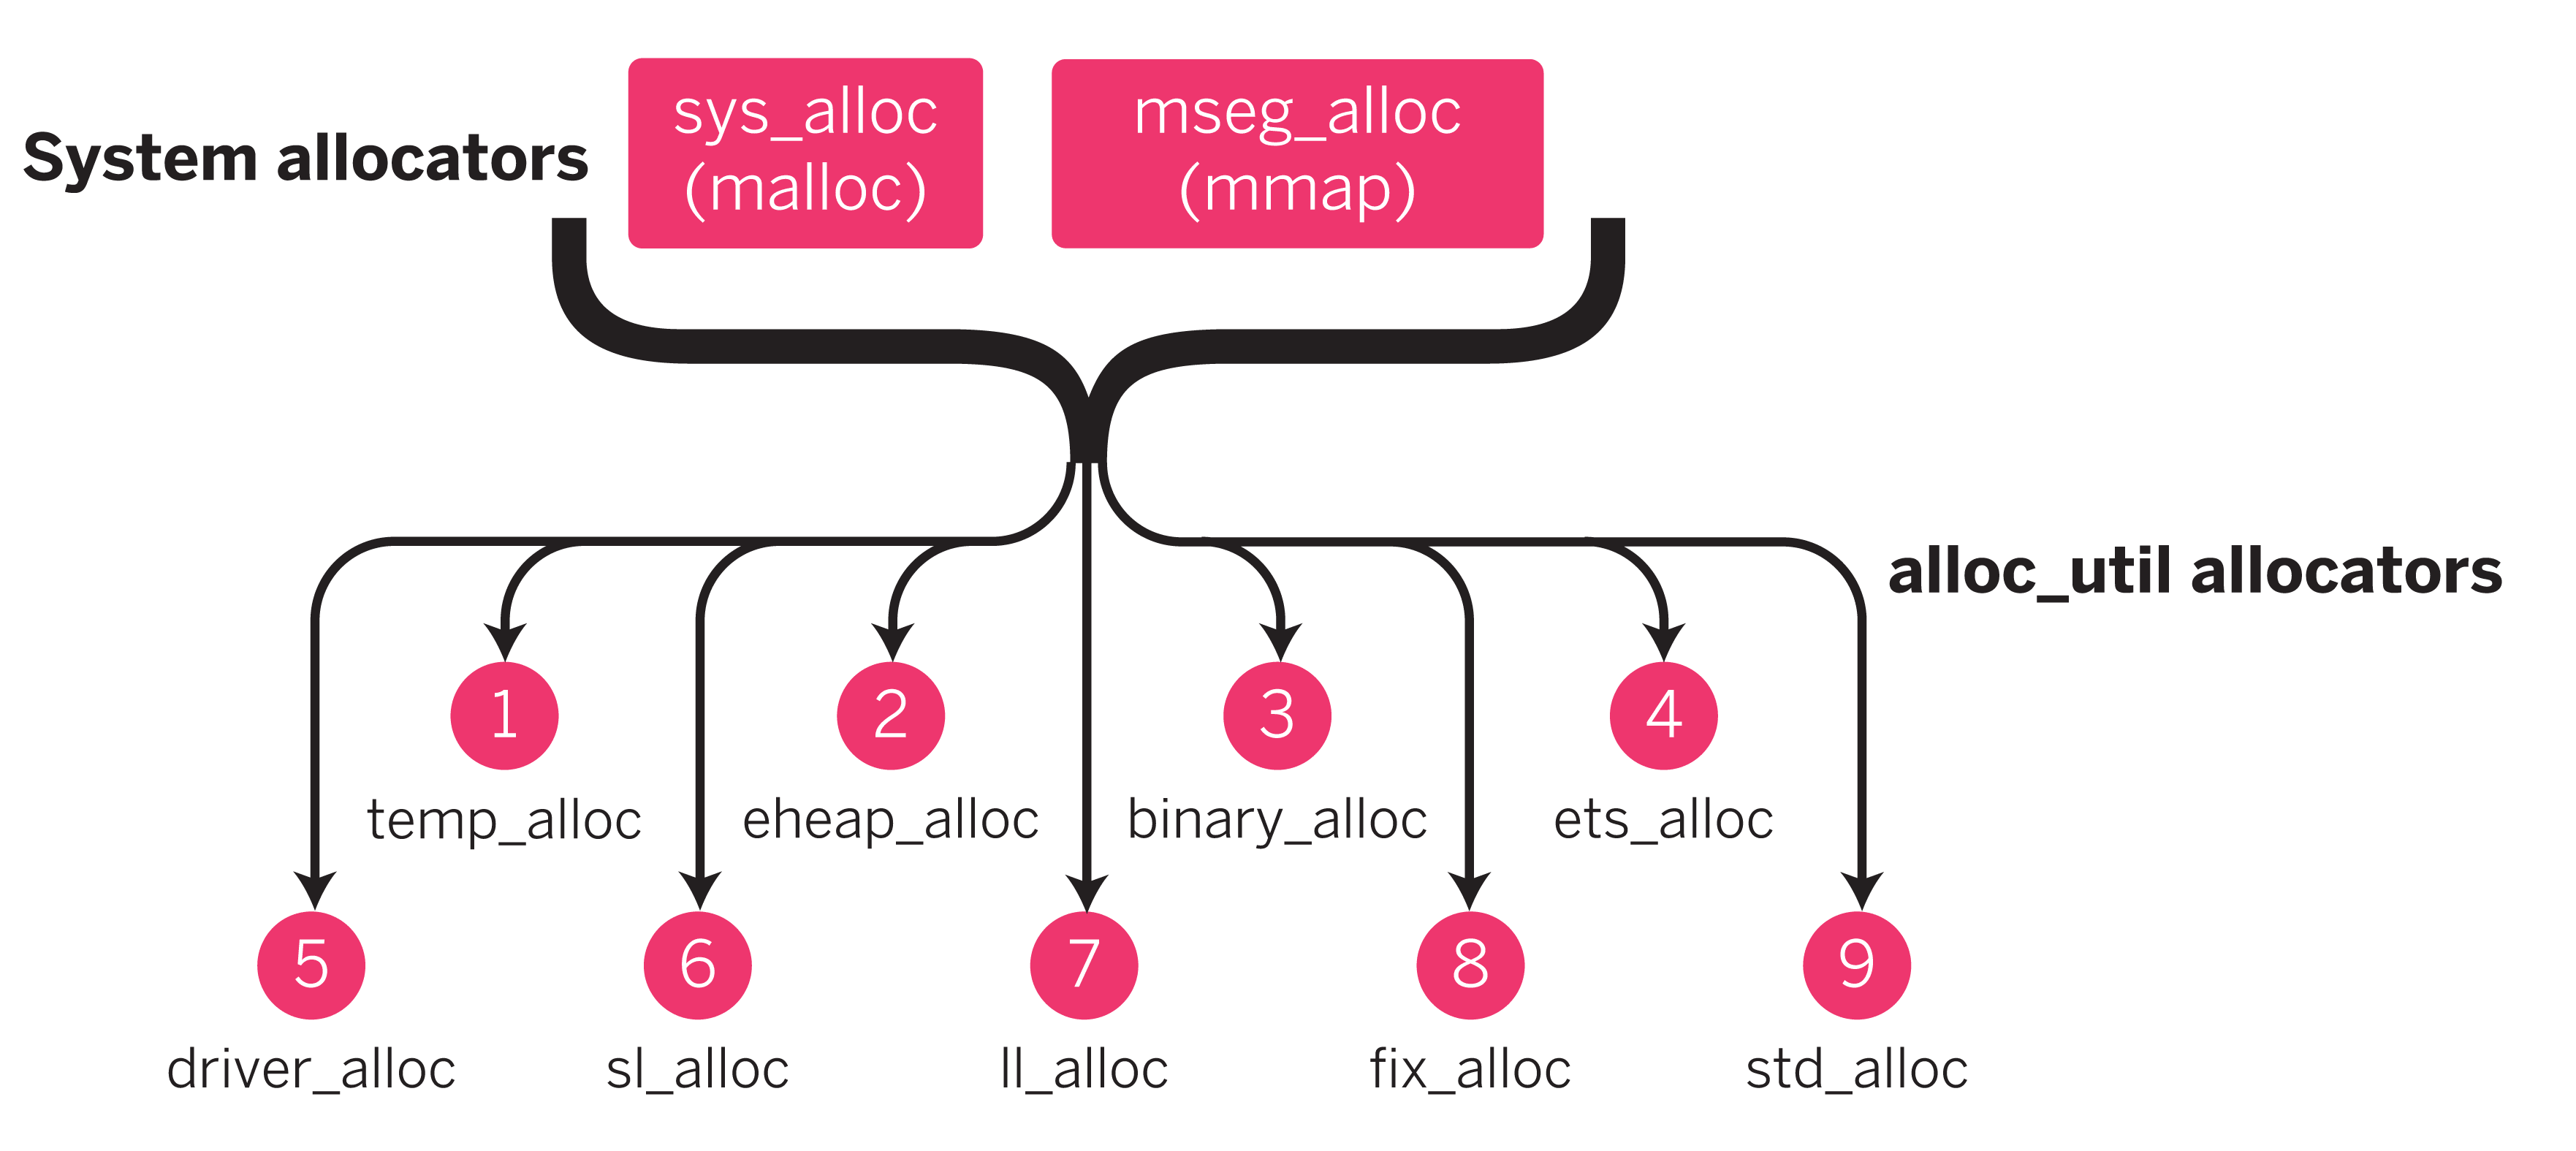
\includegraphics{memory-allocs.pdf}%
  \caption{Erlang's Memory allocators and their hierarchy. Not shown is the special \emph{super carrier}, optionally allowing to pre-allocate (and limit) all memory available to the Erlang VM since R16B03.}%
   \label{fig:allocators}
\end{figure}

\begin{enumerate*}
    \item \term{temp\_alloc}: does temporary allocations for short use cases (such as data living within a single C function call).
    \item \term{eheap\_alloc}: heap data, used for things such as the Erlang processes' heaps.
    \item \term{binary\_alloc}: the allocator used for reference counted binaries (what their 'global heap' is). Reference counted binaries stored in an ETS table remain in this allocator.
    \item \term{ets\_alloc}: ETS tables store their data in an isolated part of memory that isn't garbage collected, but allocated and deallocated as long as terms are being stored in tables.
    \item \term{driver\_alloc}: used to store driver data in particular, which doesn't keep drivers that generate Erlang terms from using other allocators. The driver data allocated here contains locks/mutexes, options, Erlang ports, etc.
    \item \term{sl\_alloc}: short-lived memory blocks will be stored there, and include items such as some of the VM's scheduling information or small buffers used for some data types' handling.
    \item \term{ll\_alloc}: long-lived allocations will be in there. Examples include Erlang code itself and the atom table, which stay there.
    \item \term{fix\_alloc}: allocator used for frequently used fixed-size blocks of memory. One example of data used there is the internal processes' C struct, used internally by the VM.
    \item \term{std\_alloc}: catch-all allocator for whatever didn't fit the previous categories. The process registry for named process is there.
\end{enumerate*}

By default, there will be one instance of each allocator per scheduler (and you should have one scheduler per core), plus one instance to be used by linked-in drivers using async threads. This ends up giving you a structure a bit like in Figure \NamedRef{fig:allocators}, but split it in \var{N} parts at each leaf.

Each of these sub-allocators will request memory from \term{mseg\_alloc} and \term{sys\_alloc} depending on the use case, and in two possible ways. The first way is to act as a multiblock carrier (\term{mbcs}), which will fetch chunks of memory that will be used for many Erlang terms at once. For each \term{mbc}, the VM will set aside a given amount of memory (about 8MB by default in our case, which can be configured by tweaking VM options), and each term allocated will be free to go look into the many multiblock carriers to find some decent space in which to reside.

Whenever the item to be allocated is greater than the single block carrier threshold (\term{sbct})\footnote{\href{http://erlang.org/doc/man/erts\_alloc.html\#M\_sbct}{http://erlang.org/doc/man/erts\_alloc.html\#M\_sbct}}, the allocator switches this allocation into a single block carrier (\term{sbcs}). A single block carrier will request memory directly from \term{mseg\_alloc} for the first \term{mmsbc}\footnote{\href{http://erlang.org/doc/man/erts\_alloc.html\#M\_mmsbc}{http://erlang.org/doc/man/erts\_alloc.html\#M\_mmsbc}} entries, and then switch over to \term{sys\_alloc} and store the term there until it's deallocated.

So looking at something such as the binary allocator, we may end up with something similar to Figure \NamedRef{fig:allocation-1-normal}

\begin{figure}
  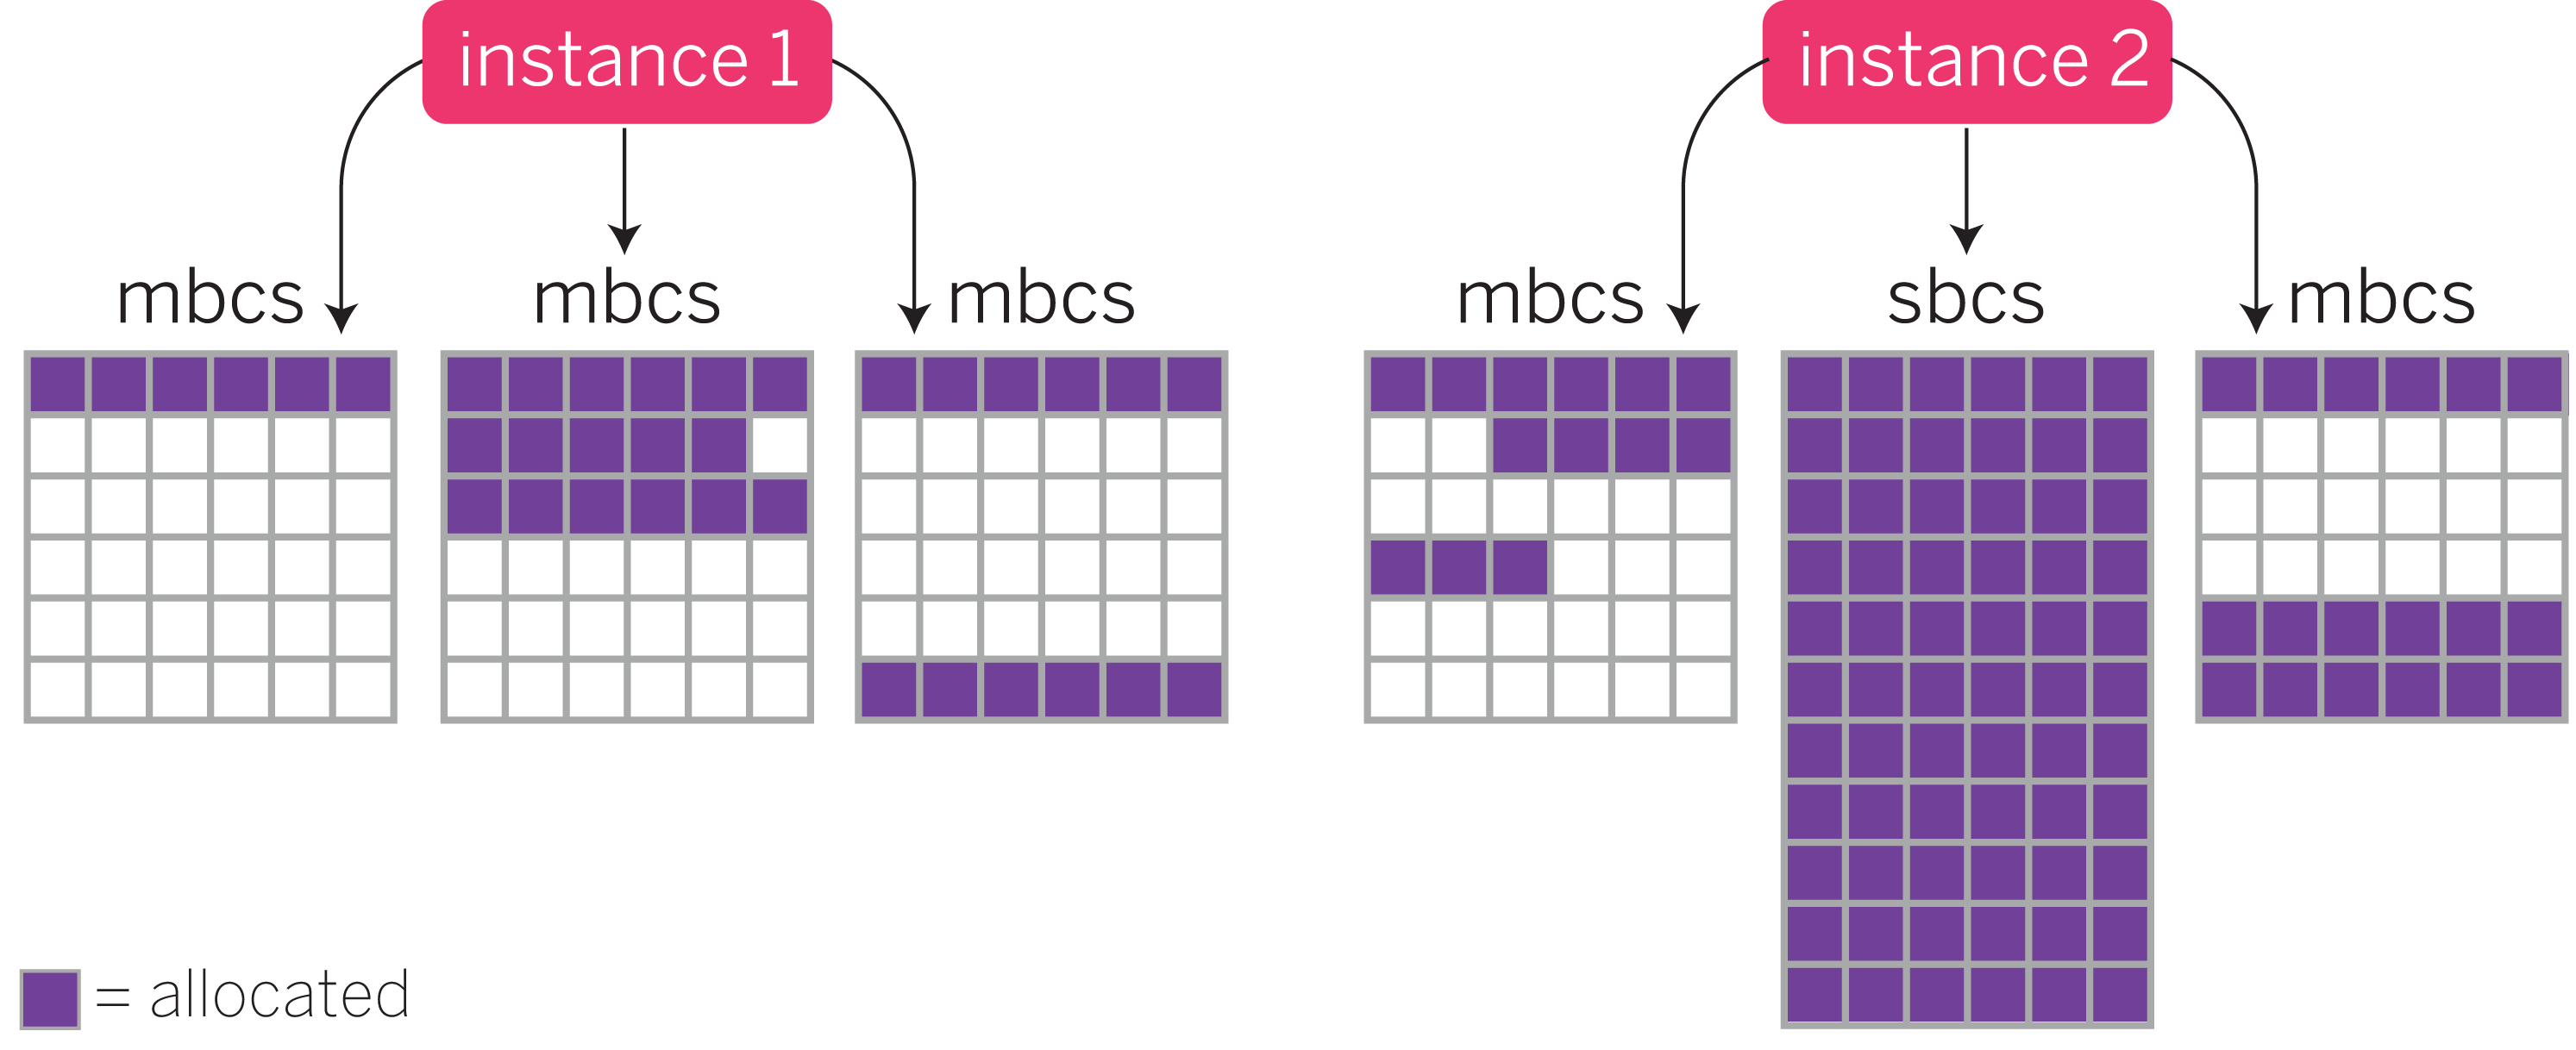
\includegraphics{allocation-1-normal.pdf}%
  \caption{Example memory allocated in a specific sub-allocator}%
   \label{fig:allocation-1-normal}
\end{figure}
\FloatBarrier

Whenever a multiblock carrier (or the first \term{mmsbc}\footnote{\href{http://erlang.org/doc/man/erts\_alloc.html\#M\_mmsbc}{http://erlang.org/doc/man/erts\_alloc.html\#M\_mmsbc}} single block carriers) can be reclaimed, \term{mseg\_alloc} will try to keep it in memory for a while so that the next allocation spike that hits your VM can use pre-allocated memory rather than needing to ask the system for more each time.

You then need to know the different memory allocation strategies of the Erlang virtual machine:

\begin{enumerate*}
    \item Best fit (\term{bf})
    \item Address order best fit (\term{aobf})
    \item Address order first fit (\term{aoff})
    \item Address order first fit carrier best fit (\term{aoffcbf})
    \item Address order first fit carrier address order best fit (\term{aoffcaobf})
    \item Good fit (\term{gf})
    \item A fit (\term{af})
\end{enumerate*}

Each of these strategies can be configured individually for each \term{alloc\_util} allocator\footnote{\href{http://erlang.org/doc/man/erts\_alloc.html\#M\_as}{http://erlang.org/doc/man/erts\_alloc.html\#M\_as}}

\begin{figure}
  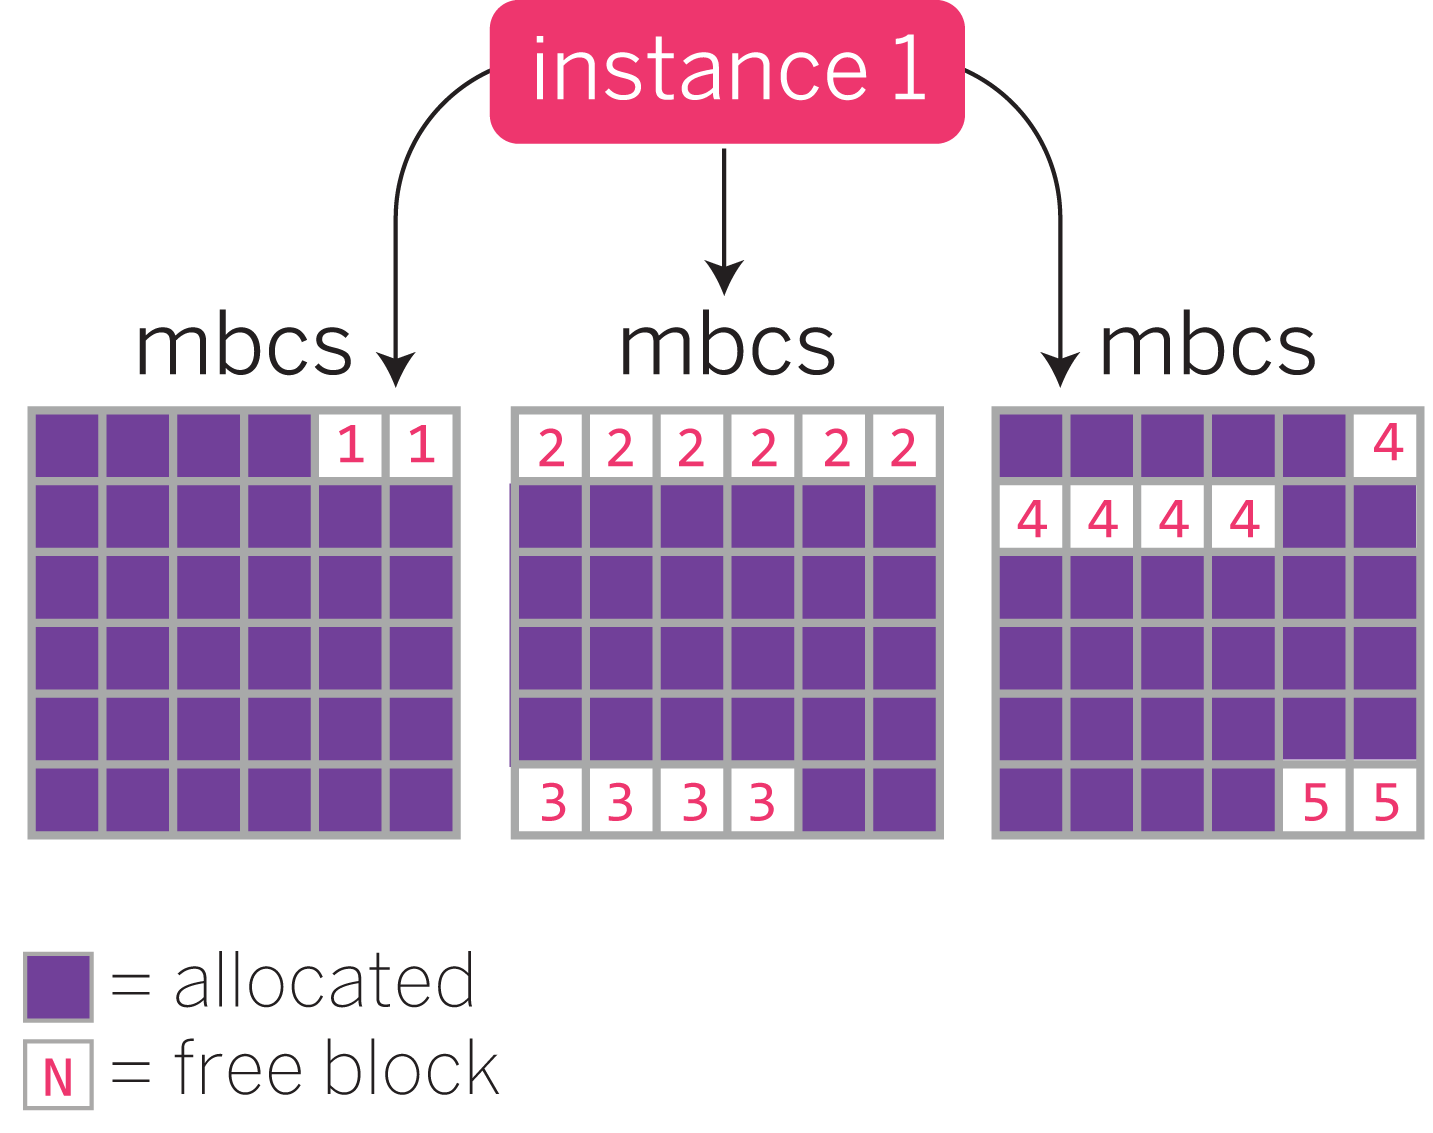
\includegraphics[max height=7cm]{allocation-strategy-1.pdf}%
  \centering%
  \caption{Example memory allocated in a specific sub-allocator}%
   \label{fig:allocation-strategy-1}
\end{figure}
\FloatBarrier

For \emph{best fit} (\term{bf}), the VM builds a balanced binary tree of all the free blocks' sizes, and will try to find the smallest one that will accommodate the piece of data and allocate it there. In Figure \NamedRef{fig:allocation-strategy-1}, having a piece of data that requires three blocks would likely end in area 3.

\emph{Address order best fit} (\term{aobf}) will work similarly, but the tree instead is based on the addresses of the blocks. So the VM will look for the smallest block available that can accommodate the data, but if many of the same size exist, it will favor picking one that has a lower address. If I have a piece of data that requires three blocks, I'll still likely end up in area 3, but if I need two blocks, this strategy will favor the first \term{mbcs} in Figure \NamedRef{fig:allocation-strategy-1} with area 1 (instead of area 5). This could make the VM have a tendency to favor the same carriers for many allocations.

\emph{Address order first fit} (\term{aoff}) will favor the address order for its search, and as soon as a block fits, \term{aoff} uses it. Where \term{aobf} and bf would both have picked area 3 to allocate four blocks in Figure \NamedRef{fig:allocation-strategy-1}, this one will get area 2 as a first priority given its address is lowest. In Figure \NamedRef{fig:allocation-strategy-2}, if we were to allocate four blocks, we'd favor block 1 to block 3 because its address is lower, whereas \term{bf} would have picked either 3 or 4, and \term{aobf} would have picked 3.

\begin{figure}
  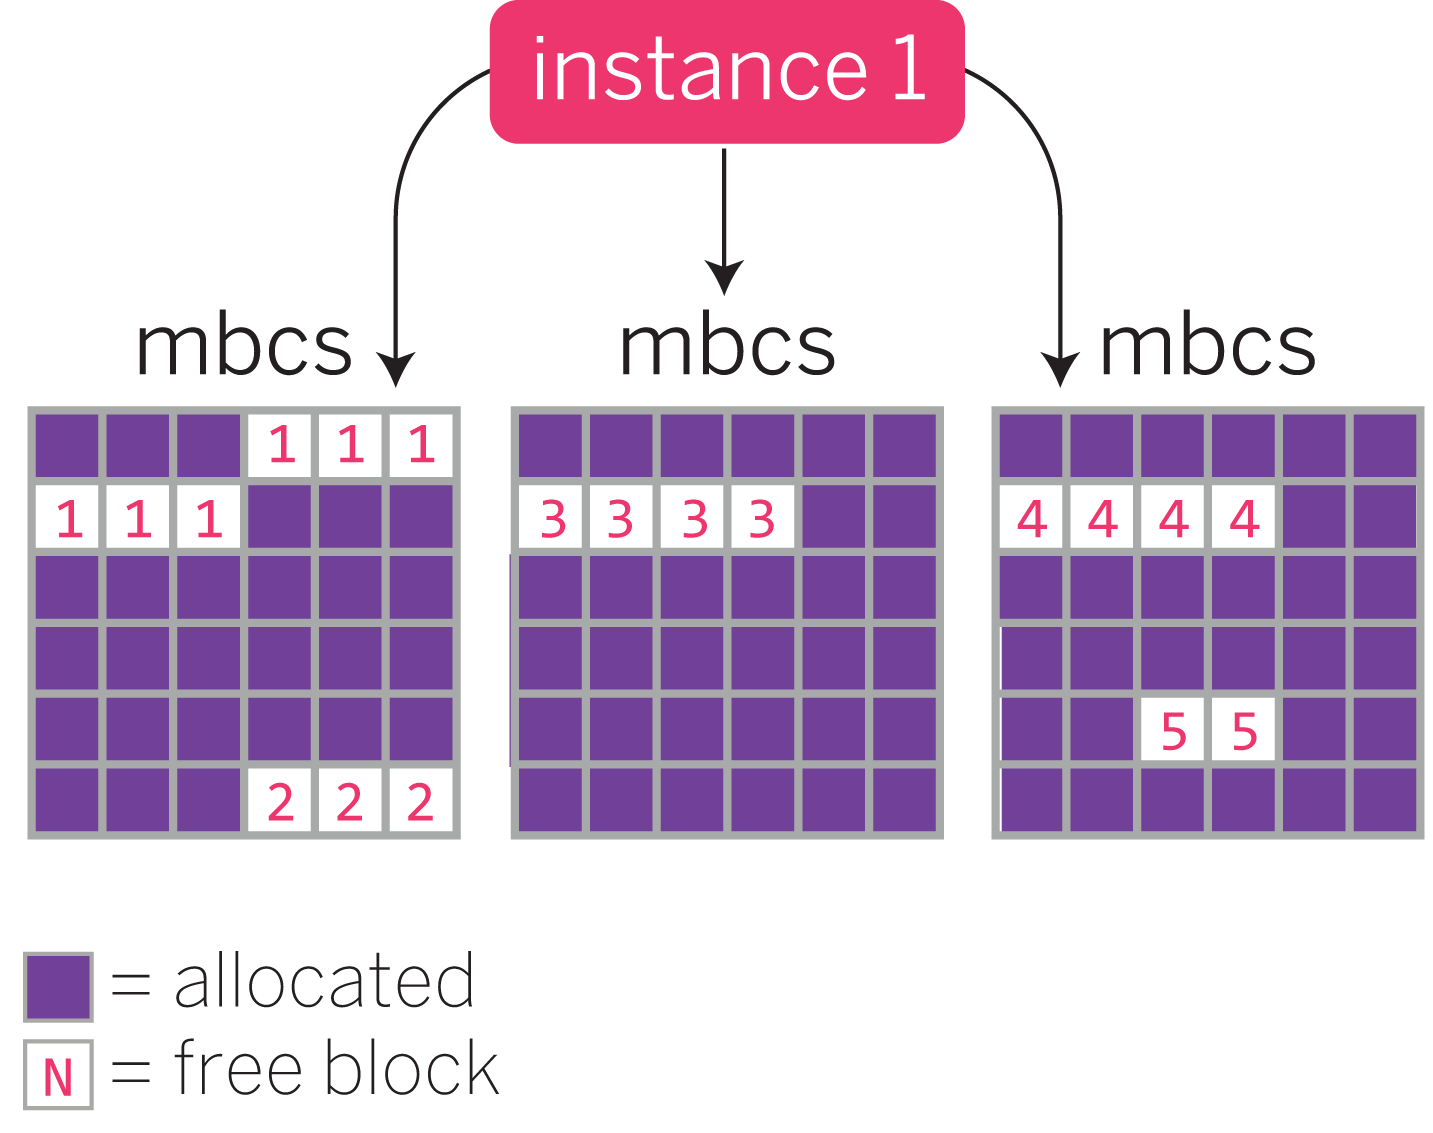
\includegraphics[max height=7cm]{allocation-strategy-2.pdf}%
  \centering%
  \caption{Example memory allocated in a specific sub-allocator}%
   \label{fig:allocation-strategy-2}
\end{figure}
\FloatBarrier

\emph{Address order first fit carrier best fit} (\term{aoffcbf}) is a strategy that will first favor a carrier that can accommodate the size and then look for the best fit within that one. So if we were to allocate two blocks in Figure \NamedRef{fig:allocation-strategy-2}, \term{bf} and \term{aobf} would both favor block 5, \term{aoff} would pick block 1. \term{aoffcbf} would pick area 2, because the first \term{mbcs} can accommodate it fine, and area 2 fits it better than area 1.

\emph{Address order first fit carrier address order best fit} (\term{aoffcaobf}) will be similar to \term{aoffcbf}, but if multiple areas within a carrier have the same size, it will favor the one with the smallest address between the two rather than leaving it unspecified.

\emph{Good fit} (\term{gf}) is a different kind of allocator; it will try to work like best fit (\term{bf}), but will only search for a limited amount of time. If it doesn't find a perfect fit there and then, it will pick the best one encountered so far. The value is configurable through the \term{mbsd}\footnote{\href{http://www.erlang.org/doc/man/erts\_alloc.html\#M\_mbsd}{http://www.erlang.org/doc/man/erts\_alloc.html\#M\_mbsd}} VM argument.

\emph{A fit} (\term{af}), finally, is an allocator behaviour for temporary data that looks for a single existing memory block, and if the data can fit, \term{af} uses it. If the data can't fit, \term{af} allocates a new one.

Each of these strategies can be applied individually to every kind of allocator, so that the heap allocator and the binary allocator do not necessarily share the same strategy.

Finally, starting with Erlang version 17.0, each \term{alloc\_util} allocator on each scheduler has what is called a \emph{\term{mbcs} pool}. The \term{mbcs} pool is a feature used to fight against memory fragmentation on the VM. When an allocator gets to have one of its multiblock carriers become mostly empty,\footnote{The threshold is configurable through \href{http://www.erlang.org/doc/man/erts\_alloc.html\#M\_acul}{http://www.erlang.org/doc/man/erts\_alloc.html\#M\_acul}} the carrier becomes \emph{abandoned}. 

This abandoned carrier will stop being used for new allocations, until new multiblock carriers start being required. When this happens, the carrier will be fetched from the \term{mbcs} pool. This can be done across multiple \term{alloc\_util} allocators of the same type across schedulers. This allows the VM to cache mostly-empty carriers without forcing deallocation of their memory.\footnote{In cases this consumes too much memory, the feature can be disabled with the options \term{+MBacul 0}.} It also enables the migration of carriers across schedulers when they contain little data, according to their needs.

\subsubsection{The Process Level}
\label{subsec:memory-process-level}

On a smaller scale, for each Erlang process, the layout still is a bit different. It basically has this piece of memory that can be imagined as one box:

\begin{VerbatimText}
[                  ]
\end{VerbatimText}

On one end you have the heap, and on the other, you have the stack:

\begin{VerbatimText}
[heap |     | stack]
\end{VerbatimText}

In practice there's more data (you have an old heap and a new heap, for generational GC, and also a virtual binary heap, to account for the space of reference-counted binaries on a specific sub-allocator not used by the process — \term{binary\_alloc} vs. \term{eheap\_alloc}):

\begin{VerbatimText}
[heap   ||    stack]
\end{VerbatimText}

The space is allocated more and more up until either the stack or the heap can't fit in anymore. This triggers a minor GC. The minor GC moves the data that can be kept into the old heap. It then collects the rest, and may end up reallocating more space.

After a given number of minor GCs and/or reallocations, a full-sweep GC is performed, which inspects both the new and old heaps, frees up more space, and so on. When a process dies, both the stack and heap are taken out at once. reference-counted binaries are decreased, and if the counter is at 0, they vanish.

When that happens, over 80\% of the time, the only thing that happens is that the memory is marked as available in the sub-allocator and can be taken back by new processes or other ones that may need to be resized. Only after having this memory unused — and the multiblock carrier unused also — is it returned to \term{mseg\_alloc} or \term{sys\_alloc}, which may or may not keep it for a while longer.

\subsection{Fixing Memory Fragmentation with a Different Allocation Strategy}

Tweaking your VM's options for memory allocation may help.

You will likely need to have a good understanding of what your type of memory load and usage is, and be ready to do a lot of in-depth testing. The \module{recon\_alloc} module contains a few helper functions to provide guidance, and the module's documentation\footnote{\href{http://ferd.github.io/recon/recon\_alloc.html}{http://ferd.github.io/recon/recon\_alloc.html}} should be read at this point.

You will need to figure out what the average data size is, the frequency of allocation and deallocation, whether the data fits in \term{mbcs} or \term{sbcs},  and you will then need to try playing with a bunch of the options mentioned in \module{recon\_alloc}, try the different strategies, deploy them, and see if things improve or if they impact times negatively.

This is a very long process for which there is no shortcut, and if issues happen only every few months per node, you may be in for the long haul. 


\section{Exercises}

\subsection*{Review Questions}

\begin{enumerate}
	\item Name some of the common sources of leaks in Erlang programs.
	\item What are the two main types of binaries in Erlang?
	\item What could be to blame if no specific data type seems to be the source of a leak?
	\item If you find the node died with a process having a lot of memory, what could you do to find out which one it was?
	\item How could code itself cause a leak?
	\item How can you find out if garbage collections are taking too long to run?
\end{enumerate}

\subsection*{Open-ended Questions}

\begin{enumerate}
	\item  How could you verify if a leak is caused by forgetting to kill processes, or by processes using too much memory on their own?
	\item A process opens a 150MB log file in binary mode to go extract a piece of information from it, and then stores that information in an ETS table. After figuring out you have a binary memory leak, what should be done to minimize binary memory usage on the node?
	\item What could you use to find out if ETS tables are growing too fast?
	\item What steps should you go through to find out that a node is likely suffering from fragmentation? How could you disprove the idea that is could be due to a NIF or driver leaking memory?
	\item How could you find out if a process with a large mailbox (from reading \term{message\_queue\_len}) seems to be leaking data from there, or never handling new messages?
	\item A process with a large memory footprint seems to be rarely running garbage collections. What could explain this?
	\item When should you alter the allocation strategies on your nodes? Should you prefer to tweak this, or the way you wrote code?
\end{enumerate}

\subsection*{Hands-On}

\begin{enumerate}
	\item Using any system you know or have to maintain in Erlang (including toy systems), can you figure out if there are any binary memory leaks on there?
\end{enumerate}
	
%%%
%%%
%%%

%%% Cognitive
%%
%% These should be done after reading the standard documentation on crash dumps referenced by the text.
%%
%% Knowledge: recall facts, terms, basic concepts
%% 
%% - What are the two main ways to find about a memory leak?
%% - What are good questions to ask about the node if you suspect a leak?
%% - Name some of the common sources of leaks in Erlang programs.
%% - What are the two main types of binaries in Erlang?
%% - What could be to blame if no specific data type seems guilty of a leak?
%% - Can Erlang's memory allocation schemes be modified or are they unchangeable without patches?
%%
%% Comprehension: organizing, comparing, translating, interpreting, giving descriptions, and stating the main ideas
%%
%% - How could you verify if a leak is caused by forgetting to kill processes, or by processes using too much memory on their own?
%% - What could cause the atom table to grow infinitely?
%% - How could code itself cause a leak?
%% - How can you find out if garbage collections are taking too long to run?
%%
%% Application: Solve problems in new situations by applying acquired knowledge, facts, techniques and rules in a different way
%%
%% - Using any system you know or have to maintain in Erlang (including toy systems), can you figure out if there are any binary memory leaks on there?
%% - A process opens a 150MB log file in binary mode to go extract a piece of information from it, and then stores that information in an ETS table. After figuring out you have a binary memory leak, what should be done to minimize binary memory usage on the node?
%% - What could you use to find out if ETS tables are growing too fast?
%%
%% Analysis: break down info, make inferences, find evidence
%%
%% - What steps should you go through to find out that a node is likely suffering from fragmentation? How could you disprove the idea that is could be due to a NIF or driver leaking memory?
%%
%% Synthesis: Compile information together in a different way by combining elements in a new pattern or proposing alternative solutions
%%
%% - How could you find out if a process with a large mailbox (from reading 'message_queue_len') seems to be leaking data from there, or never handling new messages?
%% - A process with a large memory footprint seems to be rarely running garbage collections. What could explain this?
%%
%% Evaluation: Present and defend opinions by making judgments about information
%%
%% - When should you alter the allocation strategies on your nodes? Should you prefer to tweak this, or the way you wrote code?
%% 

%%%
%%%
%%%

\chapter{CPU and Scheduler Hogs}
\label{chap:cpu-hogs}

While memory leaks tend to absolutely kill your system, CPU exhaustion tends to act like a bottleneck and limits the maximal work you can get out of a node. Erlang developers will have a tendency to scale horizontally when they face such issues. It is often an easy enough job to scale out the more basic pieces of code out there. Only centralized global state (process registries, ETS tables, and so on) usually need to be modified.\footnote{Usually this takes the form of sharding or finding a state-replication scheme that's suitable, and little more. It's still a decent piece of work, but nothing compared to finding out most of your program's semantics aren't applicable to distributed systems given Erlang usually forces your hand there in the first place.} Still, if you want to optimize locally before scaling out at first, you need to be able to find your CPU and scheduler hogs.

It is generally difficult to properly analyze the CPU usage of an Erlang node to pin problems to a specific piece of code. With everything concurrent and in a virtual machine, there is no guarantee you will find out if a specific process, driver, your own Erlang code, NIFs you may have installed, or some third-party library is eating up all your processing power.

The existing approaches are often limited to profiling and reduction-counting if it's in your code, and to monitoring the scheduler's work if it might be anywhere else (but also your code).

\section{Profiling and Reduction Counts}
\label{sec:cpu-profiling}

To pin issues to specific pieces of Erlang code, as mentioned earlier, there are two main approaches. One will be to do the old standard profiling routine, likely using one of the following applications:\footnote{All of these profilers work using Erlang tracing functionality with almost no restraint. They will have an impact on the run-time performance of the application, and shouldn't be used in production.}

\begin{itemize*}
	\item \otpapp{eprof},\footnote{\href{http://www.erlang.org/doc/man/eprof.html}{http://www.erlang.org/doc/man/eprof.html}} the oldest Erlang profiler around. It will give general percentage values and will mostly report in terms of time taken.
	\item \otpapp{fprof},\footnote{\href{http://www.erlang.org/doc/man/fprof.html}{http://www.erlang.org/doc/man/fprof.html}} a more powerful replacement of eprof. It will support full concurrency and generate in-depth reports. In fact, the reports are so deep that they are usually considered opaque and hard to read. 
	\item \otpapp{eflame},\footnote{\href{https://github.com/proger/eflame}{https://github.com/proger/eflame}} the newest kid on the block. It generates flame graphs to show deep call sequences and hot-spots in usage on a given piece of code. It allows one to quickly find issues with a single look at the final result.
\end{itemize*}

It will be left to the reader to thoroughly read each of these application's documentation. The other approach will be to run \function{recon:proc\_window/3} as introduced in Subsection \NamedRef{subsec:digging-procs}:

\begin{VerbatimEshell}
1> recon:proc_window(reductions, 3, 500).
[{<0.46.0>,51728,
  [{current_function,{queue,in,2}},
   {initial_call,{erlang,apply,2}}]},
 {<0.49.0>,5728,
  [{current_function,{dict,new,0}},
   {initial_call,{erlang,apply,2}}]},
 {<0.43.0>,650,
  [{current_function,{timer,sleep,1}},
   {initial_call,{erlang,apply,2}}]}]
\end{VerbatimEshell}

The reduction count has a direct link to function calls in Erlang, and a high count is usually the synonym of a high amount of CPU usage. 

What's interesting with this function is to try it while a system is already rather busy,\footnote{See Subsection \NamedRef{subsec:global-cpu}} with a relatively short interval. Repeat it many times, and you should hopefully see a pattern emerge where the same processes (or the same \emph{kind} of processes) tend to always come up on top.

Using the code locations\footnote{Call \expression{recon:info(PidTerm, location)} or \expression{process\_info(Pid, current\_stacktrace)} to get this information.} and current functions being run, you should be able to identify what kind of code hogs all your schedulers.

\section{System Monitors}
\label{sec:cpu-system-monitors}

If nothing seems to stand out through either profiling or checking reduction counts, it's possible some of your work ends up being done by NIFs, garbage collections, and so on. These kinds of work may not always increment their reductions count correctly, so they won't show up with the previous methods, only through long run times.

To find about such cases, the best way around is to use \function{erlang:system\_monitor/2}, and look for \term{long\_gc} and \term{long\_schedule}. The former will show whenever garbage collection ends up doing a lot of work (it takes time!), and the latter will likely catch issues with busy processes, either through NIFs or some other means, that end up making them hard to de-schedule.\footnote{Long garbage collections count towards scheduling time. It is very possible that a lot of your long schedules will be tied to garbage collections depending on your system.}

We've seen how to set such a system monitor In Garbage Collection in \NamedRef{subsubsec:leak-gc}, but here's a different pattern\footnote{If you're on 17.0 or newer versions, the shell functions can be made recursive far more simply by using their named form, but to have the widest compatibility possible with older versions of Erlang, I've let them as is.} I've used before to catch long-running items:

\begin{VerbatimEshell}
1> F = fun(F) ->
    receive
        {monitor, Pid, long_schedule, Info} ->
            io:format("monitor=long_schedule pid=~p info=~p~n", [Pid, Info]);
        {monitor, Pid, long_gc, Info} -> 
            io:format("monitor=long_gc pid=~p info=~p~n", [Pid, Info])
    end,
    F(F)
end.
2> Setup = fun(Delay) -> fun() -> 
     register(temp_sys_monitor, self()),
     erlang:system_monitor(self(), [{long_schedule, Delay}, {long_gc, Delay}]),
     F(F)
end end.
3> spawn_link(Setup(1000)).
<0.1293.0>
monitor=long_schedule pid=<0.54.0> info=[{timeout,1102},
                                         {in,{some_module,some_function,3}},
                                         {out,{some_module,some_function,3}}]
\end{VerbatimEshell}

Be sure to set the \term{long\_schedule} and \term{long\_gc} values to large-ish values that might be reasonable to you. In this example, they're set to 1000 milliseconds. You can either kill the monitor by calling \expression{exit(whereis(temp\_sys\_monitor), kill)} (which will in turn kill the shell because it's linked), or just disconnect from the node (which will kill the process because it's linked to the shell.)

This kind of code and monitoring can be moved to its own module where it reports to a long-term logging storage, and can be used as a canary for performance degradation or overload detection.

\subsection{Suspended Ports}
\label{subsec:port-system-monitors}

An interesting part of system monitors that didn't fit anywhere but may have to do with scheduling is regarding ports. When a process sends too many message to a port and the port's internal queue gets full, the Erlang schedulers will forcibly de-schedule the sender until space is freed. This may end up surprising a few users who didn't expect that implicit back-pressure from the VM.

This kind of event can be monitored by passing in the atom \term{busy\_port} to the system monitor. Specifically for clustered nodes, the atom \term{busy\_dist\_port} can be used to find when a local process gets de-scheduled when contacting a process on a remote node whose inter-node communication was handled by a busy port.

If you find out you're having problems with these, try replacing your sending functions where in critical paths with \function{erlang:port\_command(Port, Data, [nosuspend])} for ports, and \function{erlang:send(Pid, Msg, [nosuspend])} for messages to distributed processes. They will then tell you when the message could not be sent and you would therefore have been descheduled.


\section{Exercises}

\subsection*{Review Questions}

\begin{enumerate}
	\item What are the two main approaches to pin issues about CPU usages?
	\item Name some of the profiling tools available. What approaches are preferable for production use? Why?
	\item Why can long scheduling monitors be useful to find CPU or scheduler over-consumption?

\end{enumerate}

\subsection*{Open-ended Questions}

\begin{enumerate}
	\item If you find that a process doing very little work with reductions ends up being scheduled for long periods of time, what can you guess about it or the code it runs?
	\item Can you set up a system monitor and then trigger it with regular Erlang code? Can you use it to find out for how long processes seem to be scheduled on average? You may need to manually start random processes from the shell that are more aggressive in their work than those provided by the existing system.
\end{enumerate}

%%%
%%%
%%%

%%% Cognitive
%%
%% These should be done after reading the standard documentation on crash dumps referenced by the text.
%%
%% Knowledge: recall facts, terms, basic concepts
%% 
%% - What are the two main approaches to pin issues about CPU usages?
%% - Name some of the profiling tools available
%%
%% Comprehension: organizing, comparing, translating, interpreting, giving descriptions, and stating the main ideas
%%
%% - What approaches are preferable for production use? Why?
%% - Why can long scheduling monitors be useful to find CPU or scheduler over-consumption?
%%
%% Application: Solve problems in new situations by applying acquired knowledge, facts, techniques and rules in a different way
%%
%% - Can you set up a system monitor and then trigger it with regular Erlang code? Can you use it to find out for how long processes seem to be scheduled on average?
%%
%% Analysis: break down info, make inferences, find evidence
%%
%% - If you find that a process doing very little work with reductions ends up being scheduled for long periods of time, what can you guess about it or the code it runs?
%%
%% Synthesis: Compile information together in a different way by combining elements in a new pattern or proposing alternative solutions
%%
%% - A set of heavily loaded processes appear to be working fine most of the time, but eventually have their queues build up and get bogged down more and more. You suspect this might be because the process is overworked. What would you test to find the source of the issue?
%% - No process particularly stands out as being using a lot of CPU on the node. What can you do to determine whether one piece of code run many times is using too much CPU or whether the node is just purely overloaded?
%%
%% Evaluation: Present and defend opinions by making judgments about information
%%
%% - Try any of the profiling tools on any given code base. Which one do you prefer? Why?
%% 

%%%
%%%
%%%

\chapter{Tracing}
\label{chap:tracing}

One of the lesser known and absolutely under-used features of Erlang and the BEAM virtual machine is just about how much tracing you can do on there.

Forget your debuggers, their use is too limited.\footnote{One common issue with debuggers that let you insert break points and step through a program is that they are incompatible with many Erlang programs: put a break point in one process and the ones around keep going. In practice, this turns debugging into a very limited activity because as soon as a process needs to interact with the one you're debugging, its calls start timing out and crashing, possibly taking down the entire node with it. Tracing, on the other hand, doesn't interfere with program execution, but still gives you all the data you need.} Tracing makes sense in Erlang at all steps of your system's life cycle, whether it's for development or for diagnosing a running production system. 

There are a few options available to trace Erlang programs:

\begin{itemize}
	\item \module{sys}\footnote{\href{http://www.erlang.org/doc/man/sys.html}{http://www.erlang.org/doc/man/sys.html}} comes standard with OTP and allows the user to set custom tracing functions, log all kinds of events, and so on. It's generally complete and fine to use for development. It suffers a bit in production because it doesn't redirect IO to remote shells, and doesn't have rate-limiting capabilities for trace messages. It is still recommended to read the documentation for the module.
	
	\item \otpapp{dbg}\footnote{\href{http://www.erlang.org/doc/man/dbg.html}{http://www.erlang.org/doc/man/dbg.html}} also comes standard with Erlang/OTP. Its interface is a bit clunky in terms of usability, but it's entirely good enough to do what you need. The problem with it is that you \emph{have to know what you're doing}, because \otpapp{dbg} can log absolutely everything on the node and kill one in under two seconds.
	
	\item \emph{tracing BIFs} are available as part of the \module{erlang} module. They're mostly the raw blocks used by all the applications mentioned in this list, but their lower level of abstraction makes them rather difficult to use.
	
	\item \otpapp{redbug}\footnote{\href{https://github.com/massemanet/eper/blob/master/doc/redbug.txt}{https://github.com/massemanet/eper/blob/master/doc/redbug.txt}} is a production-safe tracing library, part of the \otpapp{eper}\footnote{\href{https://github.com/massemanet/eper}{https://github.com/massemanet/eper}} suite. It has an internal rate-limiter, and a nice usable interface. To use it, you must however be willing to add in all of \otpapp{eper}'s dependencies. The toolkit is fairly comprehensive and can be a very interesting install.
	
	\item \module{recon\_trace}\footnote{\href{http://ferd.github.io/recon/recon\_trace.html}{http://ferd.github.io/recon/recon\_trace.html}} is \otpapp{recon}'s take on tracing. The objective was to allow the same levels of safety as with \otpapp{redbug}, but without the dependencies. The interface is different, and the rate-limiting options aren't entirely identical. It can also only trace function calls, and not messages.\footnote{Messages may be supported in future iterations of the library. In practice, the author hasn't found the need when using OTP, given behaviours and matching on specific arguments allows the user to get something roughly equivalent.}
\end{itemize}

This chapter will focus on tracing with \module{recon\_trace}, but the terminology and the concepts used mostly carry over to any other Erlang tracing tool that can be used.

\section{Tracing Principles}
\label{sec:tracing-princples}

The Erlang Trace BIFs allow to trace any Erlang code at all\footnote{In cases where processes contain sensitive information, data can be forced to be kept private by calling \expression{process\_flag(sensitive, true)}}. They work in two parts: \emph{pid specifications}, and \emph{trace patterns}.

Pid specifications lets the user decide which processes to target. They can be specific pids, \expression{all} pids, \expression{existing} pids, or \expression{new} pids (those not spawned at the time of the function call).

The trace patterns represent functions. Functions can be specified in two parts: specifying the modules, functions, and arity, and then with Erlang match specifications\footnote{\href{http://www.erlang.org/doc/apps/erts/match\_spec.html}{http://www.erlang.org/doc/apps/erts/match\_spec.html}} to add constraints to arguments.

What defines whether a specific function call gets traced or not is the intersection of both, as seen in Figure~\NamedRef{fig:tracing-venn}.

\begin{figure}
  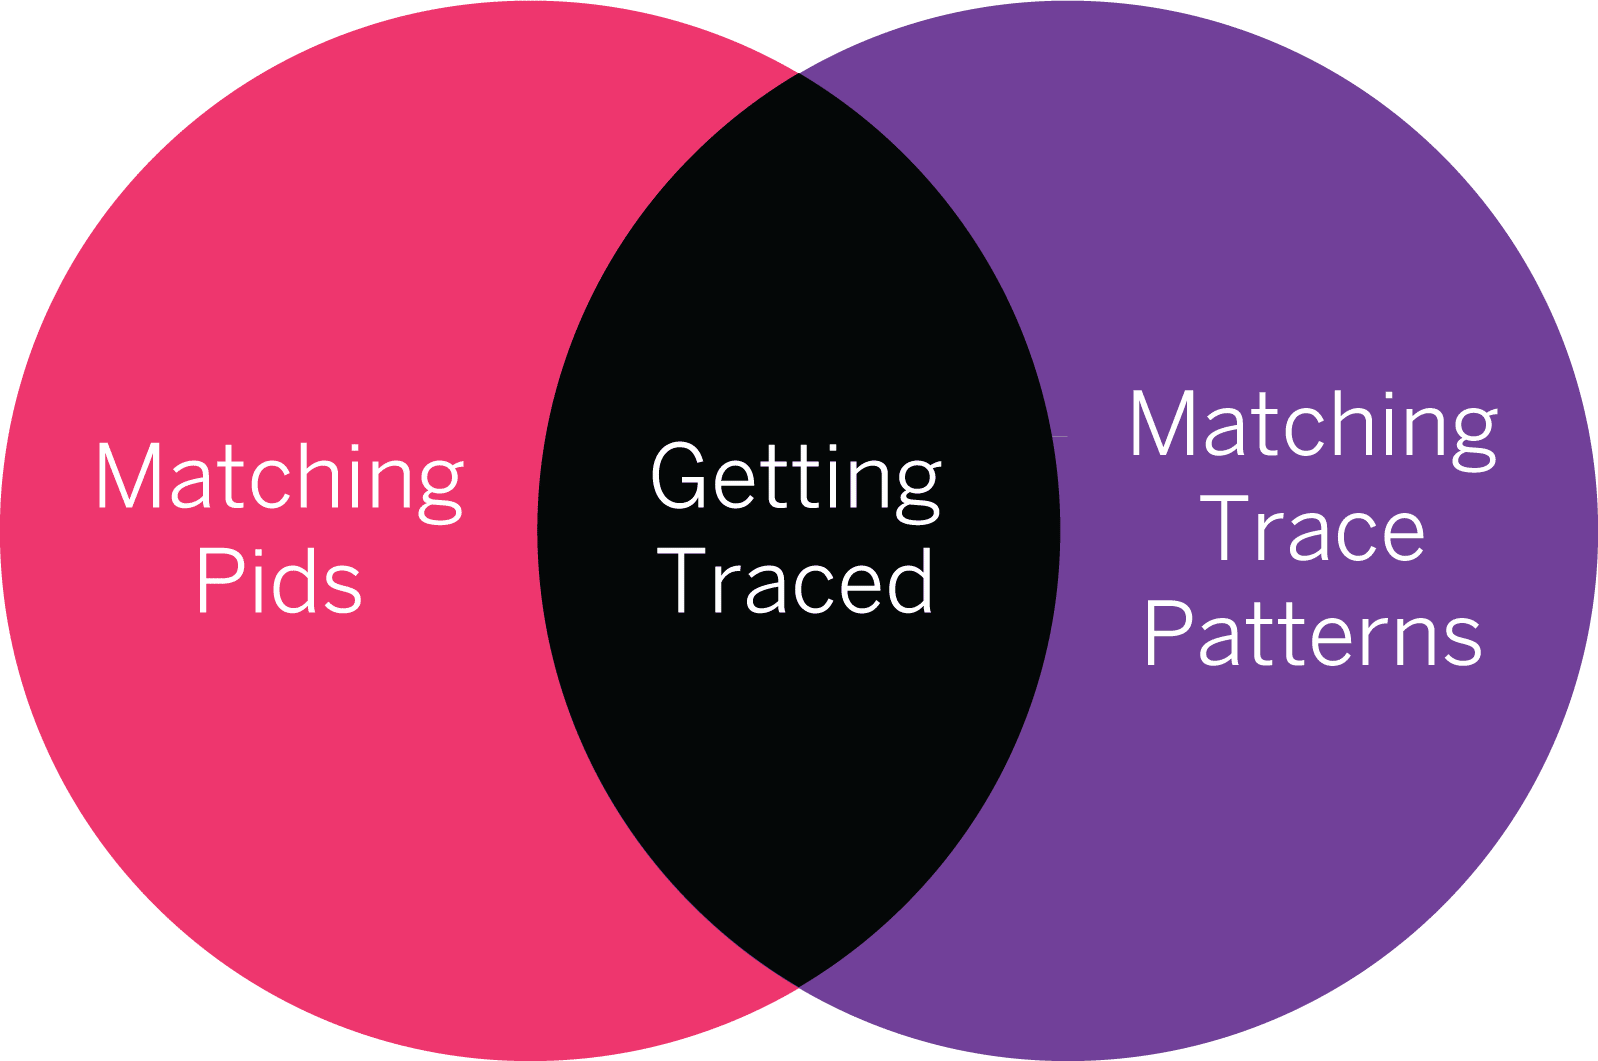
\includegraphics[max height=7cm]{tracing-venn.pdf}%
  \centering%
  \caption{What gets traced is the result of the intersection between the matching pids and the matching trace patterns}%
   \label{fig:tracing-venn}
\end{figure}

If either the pid specification excludes a process or a trace pattern excludes a given call, no trace will be received.

Tools like \otpapp{dbg} (and trace BIFs) force you to work with this Venn diagram in mind. You specify sets of matching pids and sets of trace patterns independently, and whatever happens to be at the intersection of both sets gets to be displayed.

Tools like \otpapp{redbug} and \module{recon\_trace}, on the other hand, abstract this away.
\FloatBarrier

\section{Tracing with Recon}

Recon, by default, will match all processes. This will often be good enough for a lot of debugging cases. The interesting part you'll want to play with most of the time is specification of trace patterns. Recon support a few basic ways to declare them. 

The most basic form is \expression{\{Mod, Fun, Arity\}}, where \var{Mod} is a literal module, \var{Fun} is a function name, and \var{Arity} is the number of arguments of the function to trace. Any of these may also be replaced by wildcards (\expression{'\_'}). Recon will forbid forms that match too widely on everything (such as \expression{\{'\_','\_','\_'\}}), as they could be plain dangerous to run in production.

A fancier form will be to replace the arity by a function to match on lists of arguments. The function is limited to those usable by match specifications similar to what is available in ETS\footnote{\href{http://www.erlang.org/doc/man/ets.html\#fun2ms-1}{http://www.erlang.org/doc/man/ets.html\#fun2ms-1}}. Finally, multiple patterns can be put into a list to broaden the matching scope.

It will also be possible to rate limit based on two manners: a static count, or a number of matches per time interval.

Rather than going more in details, here's a list of examples and how to trace for them.

\begin{VerbatimErl}
%% All calls from the queue module, with 10 calls printed at most:
recon_trace:calls({queue, '_', '_'}, 10)

%% All calls to lists:seq(A,B), with 100 calls printed at most:
recon_trace:calls({lists, seq, 2}, 100)

%% All calls to lists:seq(A,B), with 100 calls per second at most:
recon_trace:calls({lists, seq, 2}, {100, 1000})

%% All calls to lists:seq(A,B,2) (all sequences increasing by two) with 100 calls
%% at most:
recon_trace:calls({lists, seq, fun([_,_,2]) -> ok end}, 100)

%% All calls to iolist_to_binary/1 made with a binary as an argument already
%% (a kind of tracking for useless conversions):
recon_trace:calls({erlang, iolist_to_binary,
                   fun([X]) when is_binary(X) -> ok end},
                  10)

%% Calls to the queue module only in a given process Pid, at a rate of 50 per
%% second at most:
recon_trace:calls({queue, '_', '_'}, {50,1000}, [{pid, Pid}])

%% Print the traces with the function arity instead of literal arguments:
recon_trace:calls(TSpec, Max, [{args, arity}])

%% Matching the filter/2 functions of both dict and lists modules, across new
%% processes only:
recon_trace:calls([{dict,filter,2},{lists,filter,2}], 10, [{pid, new}])

%% Tracing the handle_call/3 functions of a given module for all new processes,
%% and those of an existing one registered with gproc:
recon_trace:calls({Mod,handle_call,3}, {1,100}, [{pid, [{via, gproc, Name}, new]}

%% Show the result of a given function call, the important bit being the
%% return_trace() call or the {return_trace} match spec value.
recon_trace:calls({Mod,Fun,fun(_) -> return_trace() end}, Max, Opts)
recon_trace:calls({Mod,Fun,[{'_', [], [{return_trace}]}]}, Max, Opts)

\end{VerbatimErl}

Each call made will override the previous one, and all calls can be cancelled with \function{recon\_trace:clear/0}.

There's a few more combination possible, with more options:

\begin{description}
	\item[\expression{\{pid, PidSpec\}}] \hfill
	
		Which processes to trace. Valid options is any of \term{all}, \term{new}, \term{existing}, or a process descriptor (\expression{\{A,B,C\}}, \expression{"<A.B.C>"}, an atom representing a name, \expression{\{global, Name\}}, \expression{\{via, Registrar, Name\}}, or a pid). It's also possible to specify more than one by putting them in a list.
		
	\item[\expression{\{timestamp, formatter | trace\}}] \hfill
	
		By default, the formatter process adds timestamps to messages received. If accurate timestamps are required, it's possible to force the usage of timestamps within trace messages by adding the option \expression{\{timestamp, trace\}}.
		
	\item[\expression{\{args, arity | args\}}] \hfill
	
		Whether to print the arity in function calls or their (by default) literal representation.
		
 	\item[\expression{\{scope, global | local\}}] \hfill
	
		By default, only 'global' (fully qualified function calls) are traced, not calls made internally. To force tracing of local calls, pass in \expression{\{scope, local\}}. This is useful whenever you want to track the changes of code in a process that isn't called with \expression{Module:Fun(Args)}, but just \expression{Fun(Args)}.
\end{description}

With these options, the multiple ways to pattern match on specific calls for specific functions and whatnot, a lot of development and production issues can more quickly be diagnosed. If the idea ever comes to say "hm, maybe I should add more logging there to see what could cause that funny behaviour", tracing can usually be a very fast shortcut to get the data you need without deploying any code or altering its readability.


\section{Example Sessions}

First let's trace the queue:new functions in any process:

\begin{VerbatimEshell}
1> recon_trace:calls({queue, new, '_'}, 1).
1
13:14:34.086078 <0.44.0> queue:new()
Recon tracer rate limit tripped.
\end{VerbatimEshell}

The limit was set to 1 trace message at most, and recon let us know when that limit was reached.

Let's instead look for all the \function{queue:in/2} calls, to see what it is we're inserting in queues:

\begin{VerbatimEshell}
2> recon_trace:calls({queue, in, 2}, 1).
1
13:14:55.365157 <0.44.0> queue:in(a, {[],[]})
Recon tracer rate limit tripped.
\end{VerbatimEshell}

In order to see the content we want, we should change the trace patterns to use a fun that matches on all arguments in a list (\term{\_}) and returns \expression{return\_trace()}. This last part will generate a second trace for each call that includes the return value:

\begin{VerbatimEshell}
3> recon_trace:calls({queue, in, fun(_) -> return_trace() end}, 3).
1

13:15:27.655132 <0.44.0> queue:in(a, {[],[]})

13:15:27.655467 <0.44.0> queue:in/2 --> {[a],[]}

13:15:27.757921 <0.44.0> queue:in(a, {[],[]})
Recon tracer rate limit tripped.
\end{VerbatimEshell}

Matching on argument lists can be done in a more complex manner:

\begin{VerbatimEshell}
4> recon_trace:calls(
4>   {queue, '_',
4>    fun([A,_]) when is_list(A); is_integer(A) andalso A > 1 ->
4>        return_trace()
4>    end},
4>   {10,100}
4> ).
32

13:24:21.324309 <0.38.0> queue:in(3, {[],[]})

13:24:21.371473 <0.38.0> queue:in/2 --> {[3],[]}

13:25:14.694865 <0.53.0> queue:split(4, {[10,9,8,7],[1,2,3,4,5,6]})

13:25:14.695194 <0.53.0> queue:split/2 --> {{[4,3,2],[1]},{[10,9,8,7],[5,6]}}

5> recon_trace:clear().
ok
\end{VerbatimEshell}

Note that in the pattern above, no specific function (\expression{'\_'}) was matched against. Instead, the fun used restricted functions to those having two arguments, the first of which is either a list or an integer greater than 1.

Be aware that extremely broad patterns with lax rate-limitting (or very high absolute limits) may impact your node's stability in ways \module{recon\_trace} cannot easily help you with. Similarly, tracing extremely large amounts of function calls (all of them, or all of \module{io} for example) can be risky if more trace messages are generated than any process on the node could ever handle, despite the precautions taken by the library.

In doubt, start with the most restrictive tracing possible, with low limits, and progressively increase your scope.


\section{Exercises}

\subsection*{Review Questions}

\begin{enumerate}
	\item Why is debugger use generally limited on Erlang?
	\item What are the options you can use to trace OTP processes?
	\item What determines whether a given set of functions or processes get traced?
	\item How can you stop tracing with \module{recon\_trace}? With other tools?
	\item How can you trace non-exported function calls?
\end{enumerate}

\subsection*{Open-ended Questions}

\begin{enumerate}
	\item When would you want to move time stamping of traces to the VM's trace mechanisms directly? What would be a possible downside of doing this?	
	\item Imagine that traffic sent out of a node does so over SSL, over a multi-tenant system. However, due to wanting to validate data sent (following a customer complain), you need to be able to inspect what was seen clear text. Can you think up a plan to be able to snoop in the data sent to their end through the \module{ssl} socket, without snooping on the data sent to any other customer?
\end{enumerate}

\subsection*{Hands-On}

Using the code at \href{https://github.com/ferd/recon\_demo}{https://github.com/ferd/recon\_demo} (these may require a decent understanding of the code there):

\begin{enumerate}
	\item Can chatty processes (\module{council\_member}) message themselves? (\emph{hint: can this work with registered names? Do you need to check the chattiest process and see if it messages itself?})
	\item Can you estimate the overall frequency at which messages are sent globally?
	\item Can you crash a node using any of the tracing tools? (\emph{hint: dbg makes it easier due to its greater flexibility})
\end{enumerate}


%%%
%%%
%%%

%%% Cognitive
%%
%% These should be done after reading the standard documentation on crash dumps referenced by the text.
%%
%% Knowledge: recall facts, terms, basic concepts
%% 
%% - Why is debugger use limited on Erlang?
%% - What are options you can use to trace OTP processes?
%%
%% Comprehension: organizing, comparing, translating, interpreting, giving descriptions, and stating the main ideas
%%
%% - What determines whether a given set of functions or processes get traced?
%% - How can you stop tracing with recon_trace?
%% - How can you trace non-exported function calls?
%%
%% Application: Solve problems in new situations by applying acquired knowledge, facts, techniques and rules in a different way
%%
%% Using https://github.com/ferd/recon_demo
%% - Can chatty processes message themselves? (can this work with registered names? Do I need to check the chattiest one and see if it messages itself?)
%% - Can you estimate the overall frequency at which messages are sent globally?
%% - Can you crash a node using any of the tracing tools? (hint: dbg makes it easier due to its flexibility)
%%
%% Analysis: break down info, make inferences, find evidence
%%
%% - When would you want to move time stamping of traces to the VM's trace mechanisms directly? What would be a possible downside of doing this?
%%
%% Synthesis: Compile information together in a different way by combining elements in a new pattern or proposing alternative solutions
%%
%% - Imagine that traffic sent out of a node does so over SSL, over a multi-tenant system. However, due to wanting to validate data sent (following a customer complain), you need to be able to inspect what was seen clear text. Can you think up a plan to be able to snoop in the data sent to their end through the 'ssl' socket, without snooping on the data sent to any other customer?
%%
%% Evaluation: Present and defend opinions by making judgments about information
%%
%% - Do you think tracing is more useful than debugging, even in development? If not, why?
%% 


%%%
%%% Tuning the VM: not a chapter yet.
%%%


%% locks!

%% you usually want the lmbcs to be at least a 5 times (if not more) bigger than the perc95

%% the binaries will still count as binary data if you move it to ets. It is only the pointer to the binary that moves from the heap to ets. (for binaries > 64 bytes)

%% Cache hits

%% Kernel Polling

%% 
\bookmarksetup{startatroot} % Split conclusion from previous Part
\addtocontents{toc}{\bigskip} % Add space in ToC
\chapter*{Conclusion}
 \markboth{\MakeUppercase{Conclusion}}{}
\addcontentsline{toc}{chapter}{Conclusion}


Maintaining and debugging software never ends. New bugs and confusing behaviours will keep popping up around the place all the time. There would probably be enough stuff out there to fill out dozens of manuals like this one, even when dealing with the cleanest of all systems. 

I hope that after reading this text, the next time stuff goes bad, it won't go \emph{too} bad. Still, there are probably going to be plenty of opportunities to debug production systems. Even the most solid bridges need to be repainted all the time in order avoid corrosion to the point of their collapse.

Best of luck to you.

\end{document}  
